\documentclass[10pt,letterpaper,oneside]{report}

\usepackage[T1]{fontenc}
\usepackage[utf8]{inputenc}
\usepackage{lmodern}
\usepackage[letterpaper,margin=0.76in,headheight=15pt,footskip=28pt]{geometry}
\usepackage{microtype}
\usepackage{amsmath,amssymb,mathtools}
\usepackage{graphicx}
\usepackage{xcolor}
\usepackage{booktabs,longtable,tabularx,array,multirow}
\usepackage{enumitem}
\usepackage{listings}
\usepackage{fancyhdr}
\usepackage{titlesec}
\usepackage{needspace}
\usepackage{xurl}
\usepackage{hyperref}
\usepackage{bookmark}
\usepackage{tikz}
\usetikzlibrary{arrows.meta,positioning,fit,calc,shapes.geometric,backgrounds}
\usepackage[most]{tcolorbox}
\usepackage{caption}
\usepackage{subcaption}
\usepackage{etoolbox}

\definecolor{Ink}{HTML}{17212B}
\definecolor{DeepBlue}{HTML}{214E78}
\definecolor{MidBlue}{HTML}{2A6F97}
\definecolor{SoftBlue}{HTML}{EAF3F8}
\definecolor{DeepGreen}{HTML}{3D6B47}
\definecolor{SoftGreen}{HTML}{EEF6EF}
\definecolor{DeepGold}{HTML}{8C6A12}
\definecolor{SoftGold}{HTML}{FBF6E6}
\definecolor{DeepRed}{HTML}{8D3A3A}
\definecolor{SoftRed}{HTML}{FBEDED}
\definecolor{DeepGray}{HTML}{48545F}
\definecolor{SoftGray}{HTML}{F4F6F7}
\definecolor{RuleGray}{HTML}{C7CED4}

\hypersetup{
  colorlinks=true,
  linkcolor=DeepBlue,
  citecolor=DeepGreen,
  urlcolor=MidBlue,
  pdfauthor={Technical walkthrough prepared for Vladimir Reshetnikov},
  pdftitle={Inside Djex and Leant: A Maintainer's Walkthrough},
  pdfsubject={Architecture, invariants, proof search, Lean integration, and maintenance guide},
  pdfkeywords={Djex, Leant, Djinn, Exference, Lean, Haskell, type-directed synthesis}
}
\urlstyle{tt}

\setcounter{secnumdepth}{3}
\setcounter{tocdepth}{2}
\setlist[itemize]{leftmargin=1.4em,itemsep=2pt,topsep=4pt}
\setlist[enumerate]{leftmargin=1.7em,itemsep=2pt,topsep=4pt}
\setlength{\parindent}{0pt}
\setlength{\parskip}{5.5pt plus 1pt minus 1pt}
\emergencystretch=2.2em

\titleformat{\chapter}[display]
  {\normalfont\bfseries\color{Ink}}
  {\filleft\Large\color{MidBlue}\chaptertitlename\ \thechapter}
  {0.5ex}
  {\titlerule[0.8pt]\vspace{1ex}\Huge}
  [\vspace{0.7ex}\titlerule]
\titleformat{\section}{\Large\bfseries\color{DeepBlue}}{\thesection}{0.7em}{}
\titleformat{\subsection}{\large\bfseries\color{DeepGreen}}{\thesubsection}{0.7em}{}
\titleformat{\subsubsection}{\normalsize\bfseries\color{DeepGray}}{\thesubsubsection}{0.7em}{}

\pagestyle{fancy}
\fancyhf{}
\fancyhead[L]{\small\nouppercase{\leftmark}}
\fancyhead[R]{\small Djex and Leant walkthrough}
\fancyfoot[C]{\thepage}
\renewcommand{\headrulewidth}{0.4pt}
\renewcommand{\footrulewidth}{0pt}

\newcommand{\code}[1]{\texttt{\detokenize{#1}}}
\newcommand{\clicode}[1]{\texttt{\detokenize{#1}}}
\newcommand{\dashdash}{\texttt{-\kern0pt-}}
\DisableLigatures{encoding = T1, family = tt*}
\newcommand{\filepath}[1]{\nolinkurl{#1}}
\newcommand{\commitid}[1]{{\ttfamily\footnotesize #1}}
\newcommand{\RepoDjex}{\href{https://github.com/VladimirReshetnikov/Djex}{Djex}}
\newcommand{\RepoLeant}{\href{https://github.com/VladimirReshetnikov/Leant}{Leant}}
\def\DjexBase{https://github.com/VladimirReshetnikov/Djex/blob/da1dd7a316975aa8a9c59022d7dbee879f67a168/}
\def\LeantBase{https://github.com/VladimirReshetnikov/Leant/blob/c3e53cee1a19a21930a64a5cb74e3926c29a7eab/}
\newcommand{\dpath}[1]{\href{\DjexBase#1}{\nolinkurl{#1}}}
\newcommand{\lpath}[1]{\href{\LeantBase#1}{\nolinkurl{#1}}}
\newcommand{\dsym}[2]{\code{#2} in \dpath{#1}}
\newcommand{\lsym}[2]{\code{#2} in \lpath{#1}}
\newcommand{\Haskell}{Haskell}
\newcommand{\Lean}{Lean 4}
\newcommand{\Djinn}{Djinn}
\newcommand{\Exference}{Exference}
\newcommand{\term}[1]{\textbf{#1}}

\newtcolorbox{invariantbox}[1][]{
  enhanced,breakable,colback=SoftGreen,colframe=DeepGreen,
  boxrule=0.7pt,arc=1.2mm,left=2mm,right=2mm,top=1.5mm,bottom=1.5mm,
  fonttitle=\bfseries,title={Invariant},#1}
\newtcolorbox{sourcebox}[1][]{
  enhanced,breakable,colback=SoftBlue,colframe=MidBlue,
  boxrule=0.6pt,arc=1.2mm,left=2mm,right=2mm,top=1.5mm,bottom=1.5mm,
  fonttitle=\bfseries,title={Source trail},#1}
\newtcolorbox{designbox}[1][]{
  enhanced,breakable,colback=SoftGold,colframe=DeepGold,
  boxrule=0.6pt,arc=1.2mm,left=2mm,right=2mm,top=1.5mm,bottom=1.5mm,
  fonttitle=\bfseries,title={Why it is designed this way},#1}
\newtcolorbox{pitfallbox}[1][]{
  enhanced,breakable,colback=SoftRed,colframe=DeepRed,
  boxrule=0.6pt,arc=1.2mm,left=2mm,right=2mm,top=1.5mm,bottom=1.5mm,
  fonttitle=\bfseries,title={Failure mode to keep in mind},#1}
\newtcolorbox{summarybox}[1][]{
  enhanced,breakable,colback=SoftGray,colframe=DeepGray,
  boxrule=0.5pt,arc=1.2mm,left=2mm,right=2mm,top=1.5mm,bottom=1.5mm,
  fonttitle=\bfseries,title={Chapter summary},#1}

\lstdefinelanguage{Haskellish}{
  morekeywords={data,type,newtype,class,instance,where,deriving,module,import,qualified,as,let,in,case,of,do,if,then,else,forall},
  sensitive=true,
  morecomment=[l]{--},
  morecomment=[s]{\{-}{-\}},
  morestring=[b]"
}
\lstdefinelanguage{Leanish}{
  morekeywords={def,theorem,example,inductive,structure,class,instance,where,match,with,fun,let,in,by,exact,apply,intro,cases,constructor,forall},
  sensitive=true,
  morecomment=[l]{--},
  morecomment=[s]{/-}{-/},
  morestring=[b]"
}
\lstset{
  basicstyle=\ttfamily\small,
  keywordstyle=\bfseries\color{DeepBlue},
  commentstyle=\itshape\color{DeepGreen},
  stringstyle=\color{DeepRed},
  frame=single,
  rulecolor=\color{RuleGray},
  backgroundcolor=\color{SoftGray},
  breaklines=true,
  keepspaces=true,
  showstringspaces=false,
  columns=fullflexible,
  xleftmargin=0.5em,xrightmargin=0.5em,
  aboveskip=6pt,belowskip=6pt
}

\tikzset{
  box/.style={draw=DeepBlue,rounded corners=2pt,fill=SoftBlue,align=center,
              minimum height=8mm,text width=29mm,inner sep=3pt,font=\small},
  greenbox/.style={draw=DeepGreen,rounded corners=2pt,fill=SoftGreen,align=center,
              minimum height=8mm,text width=29mm,inner sep=3pt,font=\small},
  goldbox/.style={draw=DeepGold,rounded corners=2pt,fill=SoftGold,align=center,
              minimum height=8mm,text width=29mm,inner sep=3pt,font=\small},
  graybox/.style={draw=DeepGray,rounded corners=2pt,fill=SoftGray,align=center,
              minimum height=8mm,text width=29mm,inner sep=3pt,font=\small},
  redbox/.style={draw=DeepRed,rounded corners=2pt,fill=SoftRed,align=center,
              minimum height=8mm,text width=29mm,inner sep=3pt,font=\small},
  flow/.style={-{Latex[length=2.1mm]},thick,draw=DeepGray},
  backflow/.style={{Latex[length=2.1mm]}-{Latex[length=2.1mm]},thick,draw=DeepGray},
  note/.style={font=\scriptsize,align=center,text=DeepGray}
}

\newcolumntype{Y}{>{\raggedright\arraybackslash}X}
\newcolumntype{L}[1]{>{\raggedright\arraybackslash}p{#1}}

\begin{document}

\hypersetup{pageanchor=false}
\begin{titlepage}
\centering
\vspace*{0.8in}
{\Huge\bfseries\color{Ink} Inside Djex and Leant\par}
\vspace{0.25in}
{\LARGE\color{DeepBlue} A Maintainer's Walkthrough of the Codebases\par}
\vspace{0.2in}
{\large Architecture, invariants, proof search, Lean integration,\par
and practical extension paths\par}
\vspace{0.8in}
\begin{tcolorbox}[width=0.86\textwidth,colback=SoftGray,colframe=RuleGray,boxrule=0.7pt,arc=1mm]
\small
\begin{tabularx}{\textwidth}{@{}L{0.18\textwidth}Y@{}}
\textbf{Djex snapshot} & \commitid{da1dd7a316975aa8a9c59022d7dbee879f67a168} \\
\textbf{Leant snapshot} & \commitid{c3e53cee1a19a21930a64a5cb74e3926c29a7eab} \\
\textbf{Relationship} & Leant's \filepath{lib/Djex} submodule is pinned to the same Djex revision. \\
\textbf{Prepared} & August 15, 2026 \\
\end{tabularx}
\end{tcolorbox}
\vfill
{\large Prepared for Vladimir Reshetnikov\par}
\vspace{0.25in}
{\small This is a source-centered walkthrough, not an API brochure. It follows the actual control flow, data ownership, validation boundaries, and maintenance seams of the pinned revisions.\par}
\end{titlepage}
\clearpage
\hypersetup{pageanchor=true}
\pagenumbering{roman}
\chapter*{Abstract}
\addcontentsline{toc}{chapter}{Abstract}

Djex and Leant form a layered type-directed synthesis system. Djex is a Haskell library and command-line environment that gives two historically distinct synthesis engines---Djinn and Exference---a common, checked vocabulary for names, kinds, types, declarations, queries, candidates, generated syntax, diagnostics, and progress. Leant is an interactive Lean shell that links against Djex, speaks to a separate Lean backend process, translates elaborated Lean goals into a deliberately restricted structural language, runs one or both synthesis engines, reconstructs Lean syntax from the generated terms, and asks Lean itself to accept or reject every proposal.

The difficult engineering is not any single search routine. It is the preservation of meaning across a chain of representations that have different type systems and different notions of evidence. A Lean expression may be dependent, universe-polymorphic, nominal, recursive, and rich in implicit arguments. The synthesis engines reason over a smaller non-dependent fragment. The bridge must therefore distinguish exact structure from opaque transport, positive evidence from negative evidence, semantic assignments from pretty-printing hints, and exhaustive search from bounded search. Most of the code exists to make those distinctions explicit and enforceable.

This document walks through that code from the outside in. It explains the build graph; the opaque authority types in Djex; Djinn's proof-producing LJT pipeline; Exference's priority-ordered typed-hole search and independent checker; the unified Djex facade and frontends; Leant's backend protocol, transactional session reconstruction, snapshots, generated \code{it} bindings, goal-fragment serializer, provider discovery, staged search policy, candidate merger, renderer, and final Lean verification; and the test suites that lock those contracts down. The last part gives end-to-end traces and change recipes intended for someone modifying or reimplementing internals rather than merely calling the public API.

\tableofcontents
\clearpage
\pagenumbering{arabic}

\chapter*{How to read this document}
\addcontentsline{toc}{chapter}{How to read this document}

The walkthrough is organized around ownership and control flow rather than alphabetically by module. Each chapter contains source trails with commit-pinned links. Line numbers are intentionally omitted: they become misleading as soon as a file changes, while symbols and file-level responsibilities usually remain meaningful across refactorings.

A reader learning the system for the first time should read Chapters~\ref{ch:joint-model}, \ref{ch:djex-map}, \ref{ch:djinn}, \ref{ch:exference}, \ref{ch:leant-model}, and \ref{ch:leant-synth-flow} in order. A maintainer debugging a failed synthesis should jump to the diagnostic funnels in Chapters~\ref{ch:render-verify} and \ref{ch:debugging}. A contributor adding new type structure should start with the change recipes in Appendix~\ref{app:change-recipes}, then read the fragment and renderer chapters carefully.

The notation \emph{authority type} means a type whose constructor is hidden and whose values can only be obtained through a validating smart constructor. This pattern is central to Djex. The notation \emph{proposal} means a term produced by search but not yet accepted by the final authority. In Djex, a proposal may first be checked by a backend-specific checker; in Leant, it must ultimately be elaborated by Lean.

\chapter*{Post-snapshot addendum:\\typed behavioral assessment}
\addcontentsline{toc}{chapter}{Post-snapshot addendum: typed behavioral assessment}
\markboth{Post-snapshot addendum: typed behavioral assessment}{}

The historical body of this walkthrough predates the typed behavioral-assessment layer. This addendum records the newer layer against the source snapshots named on the title page. Leant remains experimental: JSON shapes, names, tags, diagnostics, and output are current-tree descriptions rather than a public stability or backward-compatibility promise. The startup configuration and command-local contract file now each have one versionless schema whose explicit \code{rankingDomain} is \code{scalar} or \code{binary-product}; older numbered roots survive only in Git history and dated non-normative reports. Paths in this addendum are printed as current-tree file paths rather than through historical line-number references.

The headline is intentionally modest: the repositories now have a checked insertion seam for one finite-list-spine Length model, a scoped Z3 execution boundary, an explicit startup policy opt-in, and an optional one-command contract choice in \filepath{src/Main.hs}. Without the startup opt-in the ordinary no-option command and REPL behavior remains the exact non-strict identity path, while a requested command contract is refused before file IO. There is no claim here of general behavioral constraints, general program equivalence, a Lean-to-SMT semantics, solver-certified proofs, or automatic Z3 integration.

\section*{The current authority chain}

The newer path preserves one association across several independently checked boundaries. Reading it as a sequence is the easiest way to avoid giving a later stage authority which belongs to an earlier one.

\begin{enumerate}
  \item \textbf{Exference retains a typed occurrence.} The typed Exference runners return an opaque \code{TypedCandidate}: the historical compatibility candidate remains paired with either its exact bounded \code{TermGraph} or an explicit engine-owned absence reason. When present, the graph's erasure was checked against that compatibility candidate. \filepath{synthesis/src/Language/Haskell/Synthesis/TypedGenerated.hs} seals graph structure and typing relationships, while \filepath{synthesis/src/Language/Haskell/Synthesis/TypedCandidate.hs} prevents callers from minting a forged checked association between that graph and another compatibility candidate. Both graph parameters---the neutral type and local-identity domains---are nominal. The sealed data constructor is private and has no derived \code{Generic} reconstruction path. Public callers can construct a raw \code{TermGraphSource}, but can obtain a sealed graph from it only through the bounded validating \code{sealTermGraph} entrance.

  Both engines erase this richer view through the same \code{typedQueryResultCompatibility} function for one already-checked \code{QueryResult}. It maps only the opaque candidate payload and therefore preserves the existing evidence, progress, metadata, candidate cardinality, and ordering, while leaving graph availability unobserved and candidate tails lazy. Djinn lifts that per-result projection over its singular error channel; Exference maps it over its lazy outer result trace. The different outer cardinalities remain engine-owned rather than being hidden behind another shared wrapper.

  Leant's \filepath{src/Leant/Synth/Engine.hs} first builds one prepared semantic-origin record. Search, renderer inputs, retained Exference authority, and later exact-origin rerendering project that same record; no post-search field-for-field preparation copy exists. Each provider binding is the sole prepared owner of its private declaration inputs, renderer metadata, and ordered instantiation assignments. Preparation derives the provider declaration list and one lazy strict-map projection shared by both renderer closures; later exact-origin rerendering and inspection derive that same provider-map projection at their use edges. Djinn, Exference, and inspection derive the aggregate assignment list in binding order. One private conversion maps that exact projection through the complete source-name table for the Exference search call, preserving provider order, provider-local order, kinds, and variable identities. The typed candidate's \code{TypedCandidateSemanticSidecar} retains the exact Exference inventory/session, prepared origin and provider bindings, source-name table, session policy, and request rather than caching either the converted assignment list or a converted source goal. Package-private inspection derives both historical projections lazily; the checked handoff performs its checked source-goal conversion at the use edge. It keeps no parallel graph-key cache: the exact graph remains owned by the opaque checked candidate, and Djex fingerprints it only while sealing an actual behavioral problem. Candidate grouping and renderer filtering preserve a group sidecar only while the group still denotes the same engine candidate. During combined-engine exact-text deduplication, an earlier compatibility-only spelling may instead retain a private variant-scoped witness to the first bounded later Exference occurrence with identical bytes. That witness keeps the Exference sidecar and source renderer ordinal separate from the display group's route, display ordinal, ordering, sidecar, and sibling variants. At the verification boundary, the display route, ordinal, and text are flattened into the callback candidate, which retains that spelling's exact typed origin once rather than keeping the scheduling-only variant and a parallel origin field. A wrapper such as the classical prove-mode transformation explicitly drops both direct and recovered authority.

  \item \textbf{Lean callback acceptance is recorded, not inflated.} A rendered group carries its original renderer ordinal and semantic origin into \filepath{src/Leant/Synth/Verification.hs}. The bounded verifier tries variants lazily and mints an opaque nominal \code{Verified candidate} only when its callback returns \code{VariantAccepted}. In normal execution that callback asks the Lean backend to elaborate the generated verification program and rejects transport failures, fatal responses, diagnostics, and admitted \code{sorry} results. Nevertheless, the \code{Verified} type promises only callback acceptance at this boundary. It is not a Lean kernel proof object, behavioral evidence, or a solver certificate.

  \item \textbf{The Length handoff rechecks correspondence.} \code{prepareCheckedLengthProblem} in \filepath{src/Leant/Synth/Length/Handoff.hs} accepts the exact \code{Verified DetailedVerificationVariant}, not detached text. It fails closed unless that exact spelling has a direct or recovered typed Exference origin; engine and fitting fragments agree; no premise retargets the problem; source and search goals agree; every source variable converts through the retained name table; request contexts remain empty; and the request goal equals that derived source conversion. It then requires that the retained graph has not been lost and reruns the exact origin renderer. Every current startup or command-local contract explicitly chooses \code{cases-rejected} or \code{exact-spine-zero-step-v1} beside an exact source-ordered target-role vector. Case rejection preserves the singleton/ordinal-zero rule. The exact zero/step policy instead selects the retained renderer ordinal and checks that exact alternative against the callback-accepted text. A graph may have multiple valid Lean presentations under that explicit policy, but a recovered origin authorizes only its identical accepted spelling, not the Djinn group, a sibling variant, or another candidate.

  Only after those checks does the handoff resolve the declared unary spine and named providers through retained translation provenance. It then converts the decoded candidate-case policy and mandatory target-role vector exactly once into Djex's closed \code{LengthInterpretationPolicySource}, selecting explicit-role case rejection or explicit-role exact zero/step authority. The current Leant grammar cannot construct Djex's retained lower-level legacy case-rejection entrance without roles. Djex seals the exact inventory, spine model, provider summaries, and checked interpretation policy once into an opaque session. Leant then calls only \code{sealLengthContractInSession} and \code{sealLengthTypedCandidateProblemInSession}; it does not choose among the legacy, role-aware, and exact compatibility problem wrappers. Candidate sealing consumes that session-owned provider inventory and policy directly, revalidates the separately supplied contract through the session, and then seals the typed candidate and complete behavioral-problem identity. Renderer selection still uses the raw decoded case policy before this conversion. Thus the renderer, family, and provider demand order and the historical compatibility fingerprints stay unchanged, while target-role and case authority cannot be selected independently at later sealing stages. The exact checked provider summaries reached by symbolic interpretation flow directly into the canonical used-law identity; an independent ascending names-only list is retained only for the candidate receipt. Raw text, candidate equality, private-name spelling conventions, and a graph recovered from a rendered term are not association mechanisms.

  Successful preparation returns that sealed problem directly. The callback receipt and resolved family binding have already served their checks and are not copied into a transient handoff wrapper. During ranking, the caller-owned association is the only receipt-bearing field in each transient record: the direct compatibility path uses the verified receipt itself, while the presentation-safe path retains its batch-scoped occurrence handle without a parallel detached receipt. After the permutation seal, the accepted result keeps the sealed batch as its sole receipt owner beside an eager receipt-free summary and materializes the legacy ranked receipt view only on projection. \filepath{src/Leant/Synth/Length/Adapter.hs} fuses checked preparation with query sealing, preserving distinct handoff and query refusal stages without accepting an arbitrary detached problem.

  \item \textbf{The contract is explicit and solver-neutral.} \filepath{src/Leant/Synth/Length/Contract.hs} contains passive source vocabulary: exact Lean names for a unary zero/step spine, pre- and postconditions, optional provider laws, target roles, and a closed candidate-case policy. Leant does not infer that contract from the goal, a declaration name, or an implementation. For each provider law the caller supplies argument roles and a Length transfer expression; the exact closed provider scheme and private identity come from retained translation provenance. Successful sealing establishes consistency of the named objects with the checked handoff. It does \emph{not} establish that a caller-asserted provider law is true of the Lean implementation. Every activated startup file loads one explicit scalar or pair contract and rechecks later candidates against that fixed process-wide assertion. After activation, \texttt{:synth }\dashdash\texttt{length-contract ABSOLUTE-PATH }\dashdash\texttt{ TYPE} may instead load one command-local document whose exact root is \code{\{format, rankingDomain, contract\}}. \code{rankingDomain = scalar} selects the full scalar grammar and \code{rankingDomain = binary-product} selects the separately typed canonical-\code{Prod} grammar; it is the sole discriminator and neither nested contract admits \code{resultShape}. Both nested grammars require exact \code{targetArgumentRoles} and \code{candidateCasePolicy}, and both admit current modulo and positive-literal quotient expressions. The bounded JSON input is parsed once, with no version dispatcher, migration, or alternate-domain retry. Observed roles receive compact \code{LengthInput} indices; provider transfers retain physical provider-argument indices, so a map-shaped target can forward physical argument 1 to compact input 0 while carrying argument 0 opaquely. An unobserved role means only that the Length interpreter treats that target argument as opaque and non-inspectable; it proves nothing about inhabitance, evaluation, purity, totality, parametricity, strictness, or effects. The exact case policy likewise grants bounded model interpretation, not source termination, equivalence, proof, or pruning authority. The command reuses the already activated policy and cannot replace executable, pin, solver, artifact, replay, or ordering authority. The opaque Integration request retains the strict policy beside the lazy contract and stays on the command stack through ordinary, retry, provider, and classical lanes rather than entering REPL state, history, snapshots, or a cache. No second generic configuration aggregate or configured runner owns a duplicate pairing.

  \item \textbf{Djex seals two versioned Length problems.} The public modules below \filepath{synthesis/src/Language/Haskell/Synthesis/Semantic/Length} implement two sealed domains: \code{finite-list-spine-length/v1} and its separately typed \code{finite-binary-product-spine-lengths/v1} sibling. The product domain's public vocabulary---\code{LengthSpinePair}, \code{ValidatedLengthSpinePairCounterexample}, \code{ValidatedLengthSpinePairInputBox}, and \code{ValidatedLengthSpinePairApplicableDomain} in \filepath{synthesis/src/Language/Haskell/Synthesis/Semantic/Length/Evaluate.hs}---is nominally distinct from the scalar vocabulary, so evidence sealed under one domain cannot be presented under the other. The scalar domain interprets a declared unary zero/step spine by natural-number length, supports a bounded expression/formula language, opens the exact candidate graph against the checked target, and records the precondition, postcondition, counterexample condition, inventory, encoding, candidate, and problem fingerprints. Its additive exact-case entrance freshly re-seals a complete recursive zero/step graph against the resolved spine schema; the zero branch receives zero, the step tail receives \code{input monus 1}, and the payload remains opaque. All ordinary entrances and every other case shape fail closed. The generic behavioral envelope is the checked problem's single retained owner of the concrete encoding fingerprint; the Length-specific selector derives from it. The versioned candidate key already embeds the exact freshly checked graph fingerprint, so the interpreted candidate receipt does not retain a parallel detachable graph key. This is not a semantics for arbitrary inductives, dependent values, effects, partiality, infinite structures, or arbitrary Haskell/Lean programs.

  \item \textbf{Canonical queries precede execution.} \filepath{synthesis/src/Language/Haskell/Synthesis/Semantic/Length/SMTLib.hs} can seal a bounded canonical QF\_LIA query only from one checked Length problem. Its private typed plan remains transient through bounded rendering and structural fingerprinting; the sealed query retains only the checked problem, canonical check bytes, and complete fingerprint. Exact decoder-symbol order and optional canonical \code{get-value} bytes are rederived from the problem's sealed arity after both were already bounded and structurally fingerprinted during sealing. The fingerprint still binds the full structural plan, so emitted bytes do not become the semantic source of truth. Query construction is pure and has its own size and numeral limits. Below the domain policy, \filepath{synthesis/internal/Language/Haskell/Synthesis/Internal/SMTLib/Z3/Execution.hs} admits the reusable launch profile: explicit executable path, optional SHA-256 expectation, solver timeout and resource limit, host deadline, the controls which determine configured arguments, startup and reset bytes, empty environment, fresh-working-directory policy, and their flat canonical field slice. It owns no behavioral schema, standalone fingerprint, or fingerprint budget. \filepath{synthesis/src/Language/Haskell/Synthesis/Semantic/Length/SMTLib/Execution.hs} preserves its legacy public compatibility surface, additively exports \code{mkLengthSMTLibDescriptorBoundExecutionConfig}, \nolinkurl{mkLengthSMTLibDescriptorBoundEffectiveIDExecutableAccessExecutionConfig}, \nolinkurl{mkLengthSMTLibDescriptorBoundExecveCheckExecutableAccessExecutionConfig}, and \code{lengthSMTLibExecutionExecutableLaunchStrategy}, and wraps that profile with both Length-owned schema tags, artifact and response policy, the sole fingerprint budget, and the complete Length identity. Its digest-presence and four-way executable-launch projections are closed and byte-free; neither claims that a later executable matches or passes an access check. Constructing any policy performs no process IO and grants no solver authority. Below Length's response compatibility layer, \filepath{synthesis/internal/Language/Haskell/Synthesis/Internal/SMTLib/Response/Standard.hs} owns canonical \code{sat}/\code{unsat}/\code{unknown} bytes, bounded check-status decoding, and closed \code{unsupported}/solver-error shapes. Length maps those failures exhaustively and keeps its response schema, limits wrapper/defaults, and query-specific valuation shape. Readiness reuses only canonical \code{sat}/\code{unsat} bytes and still exact-compares complete frames. The shared layer grants no query, process, schema, or evidence authority; changing its accepted bytes or classification requires every consuming domain to revise the corresponding response/plan schema identity.

  \item \textbf{Live Z3 ownership is lexical and causal.} \filepath{synthesis/src/Language/Haskell/Synthesis/Semantic/Length/SMTLib/Live.hs} lends an opaque session only through a rank-2 callback. One capability-probed worker serves at most 64 serial queries in that lexical scope---a single shared budget of 64 scalar-plus-product transactions in total per scope, not 64 of each; no process handle, marker, ordinal, transcript, raw decoded valuation, workspace, or reusable run identity escapes. Package-private protocol and session modules use the shared \code{SMTLibCausalAction} algebra in \filepath{synthesis/internal/Language/Haskell/Synthesis/Internal/SMTLib/Causal.hs} and its domain-neutral transport driver: an exact write obligation is completed and flushed before its receiver may consume causally attributable bytes. A private Length adapter binds the process, cancellation token, and absolute deadline into the one transport handle used by that driver. Below it, \filepath{synthesis/internal/Language/Haskell/Synthesis/Internal/SMTLib/Z3/Process.hs} owns profile-driven executable observation, spawn, FIFO typed pipe events, cancellation/deadlines, and staged cleanup as one opaque schema-free runtime. The established launcher hashes and rechecks a pathname before direct spawn and therefore retains its explicit stable-namespace assumption. The additive descriptor-bound launcher instead opens the source without following its final symlink, hashes the exact bounded chunks copied into an anonymous image, checks the optional pin, seals that staged image against content and size changes, and installs the same descriptor with \code{execveat}. It never retries through the pathname. Before exec it requires working Linux \code{close\_range} for exact unrelated-descriptor closure and fails closed if that primitive is unavailable or rejects a segment; it does not substitute a scan capped by the current soft descriptor limit. This binds only the staged main-image bytes: interpreters, loaders, shared libraries, source privilege metadata, solver semantics, and reported statuses remain outside its authority. For domain identity sealing the process projects the schema-free observation and exact opaque limits from that same process. \filepath{synthesis/internal/Language/Haskell/Synthesis/Internal/Semantic/Length/SMTLib/Session/Process.hs} is now the compatibility and identity facade: it exhaustively maps the generic sanitized vocabulary and retains only that exact generic process, deriving the unchanged raw-process v2 root from its process-associated schema-free observation and process-owned limits whenever the identity is projected. It caches no parallel \code{FingerprintField}. After successful generic acquisition, the masked handoff forces the strict one-field facade and then transiently constructs and forces the derived outer root to weak head normal form before returning it, preserving the former cached-root demand point while the ordered observation-and-limit field list remains lazy and opening no new asynchronous-exception window. Legacy raw-process, ready-worker, and query-run identity bytes, schema tags, and public behavior remain unchanged. Descriptor mode instead uses additive domain-separated execution-policy, process-observation, ready-worker, scalar-run, and product-run selections; query, protocol, behavioral-problem, and evidence schemas remain unchanged. This removes cached structured authority rather than scrubbing bytes: the reversible identities still contain the exact derived raw-process field. The resulting v2 identity still binds launch and executable-observation facts without a nested copy of the complete Length policy; the scoped Session's v4 ready-worker identity still binds one complete-policy occurrence beside that raw process field. Only after readiness identity admission does the worker retain a strict query policy containing maximum queries, the query-run identity budget, protocol limits, and an opaque strict post-launch policy. That post-launch value contains exactly the per-query host deadline, artifact policy, response limits, and original complete execution-policy reversible key; it no longer contains the structured Z3 launch profile or separately projectable executable path, digest expectation, solver timeout or resource limit, argument vector, environment, or working-directory policy. The reversible key still contains the original policy bytes, so this is structured-authority narrowing rather than byte scrubbing; identity bytes, schema tags, and public behavior remain unchanged. Exact process limits come from that retained runtime for remaining-capacity and run-identity admission; capability, workspace-allocation, and ready-identity admission work is finished, while opener and Session workspace-cleanup authority stays with the enclosing scope. Query protocol and readiness capability now also share the pure cumulative cursor in \filepath{synthesis/internal/Language/Haskell/Synthesis/Internal/SMTLib/Causal/Stream.hs}. Its initial cursor starts only at offset zero; an opaque completed frame carries its hidden tail, exact policy, and charged end into an associated same-write frame, while consuming and validating boundary whitespace produces an opaque policy-and-offset token for the next-write receiver. Neither machine can detach a tail from its cumulative budget or absolute accounting position. The configured frame-total error continues to win an exact tie, and only a strictly tighter remaining cumulative budget maps to the established maximum-plus-one failure. The schema-free leaf in \filepath{synthesis/internal/Language/Haskell/Synthesis/Internal/SMTLib/Lexical.hs} owns the exact SMT-LIB whitespace predicate and canonical horizontal-tab, line-feed, carriage-return, space order used by bounded response parsing, framing, the cursor, causal attribution, process boundary draining, and unchanged protocol/capability fingerprints. Any vocabulary change must revise the affected response, framing, and plan schema identities. The schema-free receipt in \filepath{synthesis/internal/Language/Haskell/Synthesis/Internal/SMTLib/Causal/BoundaryWhitespace.hs} admits finite strict queued-drain bytes through that predicate. Process mints each nonempty receipt inside the all-or-nothing STM inspection that can still restore a non-whitespace snapshot before poison, so the driver cannot receive raw unchecked successful drain bytes. The receipt proves lexical content only; FIFO origin, bounds, nonblocking behavior, cancellation/deadline and process association, and restoration remain transport laws. For the initial adopted predecessor boundary the driver projects the receipt only after the first exact write succeeds; later completed-epoch drains preserve their existing timing. The sibling schema-free receipt in \filepath{synthesis/internal/Language/Haskell/Synthesis/Internal/SMTLib/Causal/StdoutChunk.hs} admits every nonempty strict Process read before enqueue. Empty reads remain EOF; a nonempty permitted prefix still precedes the stdout-limit terminal, while an empty prefix cannot become a successful event. The generic driver therefore cannot receive a zero-progress read or mistake an empty success for a required delimiter. This receipt proves only nonemptiness; FIFO origin, configured bounds, cancellation/deadline and process association remain transport laws, and boundary-drain rollback retains the original typed stdout receipts. The protocol fingerprint continues to bind the exact initial and optional value writes, while the private plan rederives their concatenated bytes on demand from its retained query and positional sentinels instead of caching them. Its package-private terminal decoded value owns one strict status-indexed \code{SolverObservation} rather than a separately pairable status and optional binding payload. Only the satisfiable branch can carry decoded values: status-only \code{sat} remains \code{Nothing}, the zero-input value result remains the distinct \code{Just []}, and a framed valuation is nonempty; \code{unsat} and \code{unknown} carry unit. Generic payloads remain lazy, while the opaque Length owner forces only the satisfiable \code{Maybe} spine. Session consumes that whole observation and mints one private five-way replay result for status-only satisfiable, validated vacuous satisfiable, validated framed satisfiable, unsatisfiable, or unknown. That result feeds both unchanged version-1 identity fields and a narrower completed run with one status-indexed optional-evidence observation, so invalid status/payload pairs and independent status/evidence reassociation are unrepresentable. Live copies the whole run observation once, keeps it private, and checks the exact query fingerprint before inspecting it or replaying evidence. Evidence retains normalized source-ordered inputs, while the private reversible key retains the exact bounded transcript bytes carrying the raw model; identity bytes, field order, schema, wire behavior, and public API remain unchanged, so this is structured-authority narrowing rather than byte scrubbing. Each driver invocation takes its final transcript cap from the exact sealed plan whose initial action it drives---the readiness capability plan or ordinary-query protocol plan---rather than pairing that action with a second limits/config projection. Pre-reservation query-run identity sizing uses the same protocol-plan cap. A prepared query transaction retains the exact plan, marker roles, replay limits, and deadline but neither accounting anchors nor execution authority. Atomic reservation burns its ordinal and markers, reads the last-committed stdout and stderr anchors, and mints the private nominal epoch-bound receipt accepted by execution and commit; replay projects the exact query and artifact policy from that receipt's plan. The live Session then carries the protocol plan through execution and binds its complete key into the unchanged version-1 query-run field layout; exact bounded status-frame and input-value-frame bytes remain singly stored in the causal transcript rather than being copied into the decoded branch. Positional barriers, per-query ordinals, bounded framing, whitespace-only write boundaries, deadlines, poisoning, and cleanup reject stale or misassociated output rather than scanning forward for a convenient response.

  The effective-ID descriptor sibling retains the sealed-byte branch and adds two exact raw Linux \code{faccessat2(fd, "", X_OK, AT\_EMPTY\_PATH | AT\_EACCESS)} observations on the same opened source descriptor. The first follows regular-file and any-execute-bit shape admission but precedes copying. Djex then streams each bounded chunk once to SHA-256 and a private memfd, verifies source metadata and the optional pin, assigns the staged image fixed mode \code{0500}, seals and verifies content, size, type, mode, and seal state, and rewinds it. After the deterministic test hook, the second access check runs immediately before fork, pipe, or child allocation; only then may the existing descriptor-only exec owner run. Either check shares the established cancellation and absolute opener deadline. Access denial is a closed executable rejection; a missing syscall, \code{ENOSYS}, rejection of the fixed flags with \code{EINVAL}, or another checker failure is a closed launch failure. Unsupported platforms and kernels fail only when live work demands the policy, with no mode-bit, pathname, libc-emulation, or older-launch fallback.

  These are point-in-time source VFS observations under the caller's effective filesystem credentials. They cover ordinary DAC, applicable POSIX ACLs, source-mount \code{noexec}, and inode permission hooks, but are neither a reservation nor a complete source \code{exec}/\code{bprm}/LSM/IMA/binfmt decision. The executed object is a different memfd inode whose \code{0500} mode is transport metadata: source owner/group, ACLs, set-id bits, file capabilities, extended attributes, security labels, and mount identity are not carried. Interpreters, loaders, libraries, solver semantics, and reported statuses remain unbound. The effective-ID execution, raw-process, ready-worker, and fresh/shared/scoped scalar and product run identities are domain-separated from both older launch strategies; query, protocol, behavioral-problem, quotient-receipt, and evidence identities remain unchanged. Primary semantics are documented by \href{https://man7.org/linux/man-pages/man2/access.2.html}{\code{access(2)}}, \href{https://man7.org/linux/man-pages/man2/execveat.2.html}{\code{execveat(2)}}, Linux's \href{https://github.com/torvalds/linux/blob/v6.17/fs/open.c\#L391-L547}{\code{do\_faccessat}} and \href{https://github.com/torvalds/linux/blob/v6.17/fs/namei.c\#L317-L341}{\code{inode\_permission}} paths, and the kernel's \href{https://docs.kernel.org/userspace-api/check_exec.html}{\code{AT\_EXECVE\_CHECK} documentation}.

  The fourth launch strategy adds a separately versioned Linux \code{AT\_EXECVE\_CHECK} policy instead of varying the effective-ID predecessor by host kernel. It checks the opened source with both \code{faccessat2} and descriptor-bound \code{execveat(AT\_EMPTY\_PATH | AT\_EXECVE\_CHECK)} before copying and again after the deterministic post-seal hook, then checks the staged image once more immediately before any child allocation. The staged copy is created with \code{MFD\_EXEC}, fixed to mode \code{0500}, and verified with the complete \code{F\_SEAL\_WRITE}, \code{F\_SEAL\_GROW}, \code{F\_SEAL\_SHRINK}, \code{F\_SEAL\_FUTURE\_WRITE}, \code{F\_SEAL\_EXEC}, and \code{F\_SEAL\_SEAL} set. A stock Linux 5.15 runtime therefore returns a closed launch-unavailable failure before staging; a compatible Linux 6.14-or-newer kernel may admit the checks, but there is no predecessor, pathname, or weakened-seal fallback. The check deliberately does not resolve file format or interpreter dependencies and grants no source-authorization transfer, credential-transition, binfmt/bprm, loader, library, solver, or result authority. Its execution-policy, raw-process, ready-worker, and fresh/shared/scoped scalar and product run identities are additive and domain-separated; every older identity byte and the query, protocol, behavioral-problem, monus-receipt, and evidence identities remain literal.

  The ordinary-query plan sealer consumes the associated post-launch policy rather than the full structured \code{LengthSMTLibExecutionConfig}. After validation and fingerprint sealing, \code{LengthSMTLibProtocolPlan} retains only the exact artifact-policy and bounded-response-limit projections, nominal query, cumulative cursor policy, positional barriers, and reversible plan key needed by later protocol consumers. That unchanged plan key still embeds the original complete execution-policy key; launch-profile, digest, solver-control, deadline, environment, and working-directory facts are not retained as separate structured plan authority.

  The stdout receipt is projected only at the driver's existing receiver-feed and post-epoch boundary-collection edges.

  For surviving positive-literal modulo and quotient nodes, Djex never emits SMT-LIB \code{mod} or \code{div}. It allocates deterministic private quotient/remainder witnesses in one mixed preorder, hoists only Euclidean linear equations and Natural bounds into QF\_LIA, and keeps those witnesses out of \code{get-value} and evidence presentation. Modulo projects the remainder, quotient projects the Natural floor quotient, and replay independently recomputes either operation from original inputs.

  Under legacy path launch, the executable digest remains a bounded pre-spawn pathname observation and does not attest the executed image. Under descriptor launch, the digest names the sealed staged main-image bytes passed to \code{execveat}, but still does not attest an interpreter, loader, shared library, or solver semantics. The live facade exposes only sanitized status, association, evidence, and closed failure classes. Under the explicit CLI opt-in, the child solver is a fourth computational domain whose session authority is lent only for one dynamic ranking scope; the default no-option three-domain runtime described in Chapter~\ref{ch:joint-model} remains accurate. A worker belongs to one attempted ranking batch. Cleanup is owned and attempted when the scope exits, incomplete cleanup is reported, and no worker becomes long-lived interactive session state.

  \item \textbf{Status indexes any evidence.} \code{sat}, \code{unsat}, and \code{unknown} are all retained only as \code{HeuristicRankingOnly} solver observations. From protocol completion through Session commit and the publicly opaque Live owner, one status-indexed \code{SolverObservation} replaces a separately pairable status and optional payload: only the satisfiable branch can contain decoded bindings or replayed evidence, while the \code{unsat} and \code{unknown} branches contain unit. Generic observation payloads remain lazy, and the opaque Length owners force only the satisfiable \code{Maybe} spine; status-only \code{sat} remains \code{Nothing}, while the zero-input values result remains the distinct \code{Just []}. Status and conservative strength are derived from the closed family and status constructor without inspecting artifact payloads or copying either fact into parallel fields. In particular, \code{unsat} is relative to the bounded encoding and is neither a solver certificate nor pruning authority; status-only \code{sat} has no model evidence. Under the input-values policy, a satisfiable response can yield evidence only after exact symbol decoding and an independent concrete natural-number replay against the checked Length problem. The whole Live observation has no public projection. Djex's \code{replayLengthSMTLibLiveQueryObservation} checks the returned query fingerprint before inspecting it, then replays any opaque evidence once more against the exact behavioral problem retained by the sealed query. Leant accepts a \code{ValidatedLengthCounterexample} only through that gate; Djex's public Live API and query-run identity bytes remain unchanged, and the heavier handoff is transient after query sealing.

  Even that receipt is deliberately limited. It says that one bounded finite-spine natural assignment violates the sealed postcondition under the sealed precondition and model. If the candidate used named provider laws, the receipt explicitly remains conditional on those assumptions. It is not a concrete Lean value, a source-level execution, a solver-soundness theorem, or a kernel proof.

  After the occurrence seal, \filepath{src/Leant/Synth/Length/Presentation.hs} traverses each whole materialized ranked receipt and derives one opaque candidate-text-plus-note value. Main uses that one ordered list for Lean bindings, splices, and \code{itN} output; it never zips a detached evidence list back to candidates by spelling or index. Independently replayed counterexamples, independently completed bounded-positive input-box receipts, and current applicable-domain receipts produce subordinate notes in both the scalar and canonical-\code{Prod} domains. A counterexample note calls the receipt replayed and model-relative and renders a bounded summary of observed input and result spine lengths. A bounded-positive note reports the checked bounded region and its checked and applicable assignment counts, stating explicitly when zero applicable assignments make the result vacuous. Applicable-domain presentation uses only \code{renderLengthApplicableDomainValidationNote} or \code{renderLengthSpinePairApplicableDomainValidationNote} and includes the canonical maxima-antichain prefix, box and visit counts, unique and applicable assignments, and basis. All note forms reduce a provider-backed basis to the number of assumed laws. None projects the receipt's private provider-name list, attributes positive evidence to raw \code{unsat}, or makes a Lean, proof, correctness, or Z3-attestation claim.

  \item \textbf{Assessment may reorder but never prune.} The package-private implementation in \filepath{src/Leant/Synth/Length/Ranking/Internal.hs} first productively admits at most 64 candidates and completes all pure candidate/query preparation before opening a worker. Programmatic policies may leave completed positive receipts neutral or enable either non-vacuous preference independently. The current startup policy enables both preferences and the recursive piecewise-affine validator. Its stable order is non-vacuous applicable-domain evidence, non-vacuous explicit-box evidence, neutral or vacuous assessments, then independently replayed counterexamples. Original order is retained inside every partition and every callback receipt remains present. Contract-only files select no ranking policy. Any returned session, query, fingerprint-association, or evidence-replay failure discards partial live assessments and restores literal original order: eligible candidates become \code{Unassessed}, while actual pure preparation refusals retain their bounded refusal class.
  Pure candidate-local preparation refusals use ten fixed payload-free classes: unsupported route, typed authority unavailable, candidate association rejected, rendering association rejected, spine binding unavailable, provider binding unavailable, session rejected, contract rejected, candidate semantics rejected, and query construction rejected. Their fixed codes reveal only the phase. The classifier does not evaluate or copy renderer text, source names, types, graph identities, or nested Djex errors from a raw refusal into that diagnostic; the exact verified receipt and semantic sidecar remain reachable only through the caller-owned association. Such a pre-execution refusal survives atomic batch fallback; a candidate which reached execution gets no fabricated preparation reason. Refusal classes are diagnostics, not behavioral strength and not ranking input.

  \item \textbf{A generative seal protects the final permutation.} \filepath{src/Leant/Synth/PostVerification.hs} introduces a fresh rank-2 epoch for the exact opaque \code{VerificationBatch}. An assessor may reorder only the supplied private occurrence handles. The seal productively bounds both lists and requires equal length, in-range indices, and no duplicate occurrence, so it cannot omit, manufacture, duplicate, or substitute an equal-valued candidate. Equal payloads remain distinct occurrences. The Length adapter in \filepath{src/Leant/Synth/Length/PostVerification.hs} carries each assessment with its batch-scoped handle through ranking and seals the handle permutation before erasing that association. The accepted result retains that sealed batch as its sole verified-receipt owner beside an eager receipt-free index/assessment/failure summary; it materializes the legacy receipt-bearing ranking report only when that compatibility view is requested.
  \item \textbf{The current startup route fixes one advanced policy.} The versionless startup decoder composes the recursive piecewise-affine applicable-domain validator, both non-vacuous preferences, componentwise-lexicographic simplification, deferred opening, and one scoped usable-work deadline. It completes admission and preparation, then runs each candidate's MRU $\rightarrow$ recursive-domain $\rightarrow$ origin prefix before IO. An all-pure batch opens no process; the first live miss opens one lexical session, executes that head once without repeating its pure prefix, and processes the suffix in the same session. Every counterexample from those pure sources, live replay, or the post-\code{unsat} box crosses the same query-owned simplification seam, and only its final vector enters the domain-local MRU. Any indexed failure atomically restores original order and clears earlier evidence and occurrence-attached metadata; a pre-open failure launches nothing. Contract-only documents use one current versionless domain-selected schema and carry no ranking or execution policy.
\end{enumerate}

\begin{invariantbox}[title={Current post-verification invariant}]
The only candidate batch eligible for sealed post-verification presentation and reordering through the Length adapter is the exact callback-accepted batch. Under the historical/default policy, the only reason to move an occurrence is an independently replayed counterexample for the exact retained Exference graph and the canonical scalar or pair query sealed from its checked handoff; it moves stably behind neutral candidates. That replayed counterexample need not come from a live solver response: a hit in the four-entry MRU input replay bank or the query-owned all-zero origin probe yields the same independently validated receipt with no live Z3 query at all. Under an explicit non-vacuous-positive preference---which exists on two axes, the finite input box and the complete applicable domain---an independently completed positive receipt for that same query may instead move stably ahead of the neutral partition only when its applicable-assignment count is greater than zero; a zero-applicable receipt remains neutral, and exact counterexamples remain stably last. No raw solver status moves or removes a candidate: in particular, \code{unsat} only schedules the independent finite-box traversal. A complete bounded permutation is sealed before presentation. Candidate text and any counterexample or bounded-positive semantic note are then erased from the same whole ranked receipt into one presentation value, so equal spellings cannot exchange evidence. Association-free compatibility runners remain lower-level reports and do not themselves grant presentation authority.
For the current startup route, the same invariant has two positive partitions: a non-vacuous recursive applicable-domain receipt precedes a non-vacuous explicit-box receipt; neutral and vacuous assessments follow; counterexamples remain last. Each counterexample has first crossed the query-owned simplification seam, and the final vector is the only vector offered to the domain-local MRU. Deferred lifecycle state is not evidence and cannot enter presentation.
\end{invariantbox}

\section*{The binary-product mirror and the newer ranking mechanics}

The canonical-\code{Prod} path is carried by a module quartet that mirrors the scalar ranking stack: \code{Leant.Synth.Length.SpinePair.Ranking}, \code{Leant.Synth.Length.SpinePair.Ranking.Internal}, \code{Leant.Synth.Length.SpinePair.PostVerification}, and \code{Leant.Synth.Length.SpinePair.PostVerification.Internal}. On the Djex side, \filepath{synthesis/internal/Language/Haskell/Synthesis/Internal/Semantic/Length/SMTLib/Protocol/SpinePair.hs} is deliberately thin: the scalar and product protocol modules now share one phase machine, framing validation, write rendering, and fingerprint construction, parameterized by the \code{LengthSMTLibProtocolIdentity} record in \filepath{.../Semantic/Length/SMTLib/Protocol.hs}. The SpinePair wrapper contributes only what distinguishes the product domain---its schema tags, plan fingerprint role, and exact product-query projections---while its nominal plan, receiver, and decoded types remain distinct from their scalar siblings, so evidence sealed under one domain cannot be presented under the other even when the rendered wire bytes coincide.

Before any later live call inside one ranking scope, the internal ranking modules consult a bounded MRU input replay bank: at most four exact counterexample input vectors, kept newest-first with exact-vector deduplication. Each vector is independently validated and replayed against that candidate's own checked query; a hit yields an ordinary validated counterexample receipt, avoids one live query, and promotes the vector to the MRU end. The bank stores only input vectors---no cached verdicts, solver statuses, receipts, or proofs---and it never crosses a ranking batch.

When the replay bank yields no hit---at most four misses---the current startup policy probes the canonical all-zero input vector owned by that exact query; lower-level programmatic policies may enable the same probe independently. A hit enters the same validated receipt and MRU path; an ordinary miss simply proceeds to live execution and carries no positive or negative authority of its own.

Applicable-domain validation is the second positive axis beside the finite input box: one independent, query-owned exhaustive recursive piecewise-affine traversal for the scalar or binary-product domain. Leant exposes only \code{enableLengthRankingApplicableDomainValidation}. Djex exposes the short \code{validateLengthProblemApplicableDomain} and \code{validateLengthSpinePairProblemApplicableDomain} checked-problem validators plus \code{validateLengthSMTLibQueryApplicableDomain} and \code{validateLengthSpinePairSMTLibQueryApplicableDomain}, together with the short receipt and error families. Direct, affine, relational, strict, quotient, extrema, monus, Boolean-union, and atomic analyses are ordered private fallbacks inside that validator, not public strategy choices. Their former public builders, receipts, assessments, failures, renderers, and schema tags were deleted without aliases or migration because the projects are experimental and promise no stability or backward compatibility. Contract-only files never select ranking policy, and, like the input box, the external solver status itself never becomes the evidence.

\section*{Djinn uses the envelope without inventing graph authority}

Djinn now exposes \code{DjinnTypedCandidate} and \code{DjinnTypedResult}, with typed counterparts of its ordinary, provider-candidate, assignment, and kinded-assignment runners in \filepath{djinn/src-core/Language/Haskell/Djex/Djinn.hs} and \filepath{djinn/src-core/Djinn/Core.hs}. The legacy runners lift the shared one-way \code{typedQueryResultCompatibility} projection over those singular typed paths; Exference uses the same per-result edge inside its lazy result trace. Final candidate keys are allocated only after proof checking, deduplication, and any configured final ordering step, so future typed occurrence identities need not depend on discarded proof-plan ordinals.

This common result shape is not a license to synthesize a graph. Djinn's independently checked LJT evidence precedes source-name restoration, provider rewriting, instantiation-evidence lowering, visible type applications, pattern refinements, simplification, and final naming; structural formula expansion has also discarded source distinctions needed for a shared typing derivation. Every current Djinn typed candidate therefore reports the explicit absence \code{DjinnTermGraphSourceTypingContextUnavailable}. The absence is a capability result, not a search failure and not weaker logical evidence.

The reserved future graph type retains variable role. The literal right-hand side of \code{DjinnTermGraphTypeVariable} is \code{SharedType.Variable HSymbol}; \code{DjinnTermGraphType} then applies \code{SharedType.Type} to that alias. This differs from the historical role-erased compatibility type. Constructing it soundly will require retained source authority and a bounded bidirectional check of the final generated clause with exact compatibility erasure. Until such a graph exists, Djinn candidates are not eligible for the Length handoff, Z3 ranking, or any other graph-based behavioral contract. Code must not replace the explicit absence by guessed annotations reconstructed from final syntax.

\section*{Module map for the added foundation}

The following paths are current-branch source locations, not links into the pinned walkthrough snapshots.

\begin{longtable}{@{}L{0.43\textwidth}L{0.53\textwidth}@{}}
\toprule
\textbf{Djex path} & \textbf{Authority or responsibility} \\
\midrule
\endhead
\filepath{synthesis/src/Language/Haskell/Synthesis/TypedGenerated.hs} & Bounded typed term graph, checked erasure, nominal type/local domains, and graph construction limits. \\
\filepath{synthesis/src/Language/Haskell/Synthesis/TypedGenerated/Fingerprint.hs} & Allocation-insensitive structural fingerprint for a sealed graph. \\
\filepath{synthesis/src/Language/Haskell/Synthesis/TypedCandidate.hs} & Public opaque typed-candidate facade and shared evidence-preserving compatibility projection for one checked query result. \\
\filepath{synthesis/internal/Language/Haskell/Synthesis/Internal/TypedCandidate.hs} & Private representation, nominal roles, checked construction seam, lazy selectors, and canonical implementation of the per-result projection. \\
\filepath{exference/src-core/Language/Haskell/Djex/Exference.hs} & Public Exference typed runners and checked-candidate projection. \\
\filepath{exference/src-core/Language/Haskell/Exference/Core/Internal/ExpressionCheck.hs} & Private typed reconstruction which admits completed Exference expressions and checks graph erasure before graph projection. \\
\filepath{djinn/src-core/Language/Haskell/Djex/Djinn.hs} & Public Djinn typed runners and compatibility projections. \\
\filepath{djinn/src-core/Djinn/Core.hs} & Proof-checked result associations, final ranking/deduplication, and explicit typed graph absence. \\
\filepath{djinn/src-internal/Djinn/Internal/CheckedCandidate.hs} & Private validated-candidate association and post-ranking keyed projection seam. \\
\filepath{synthesis/src/Language/Haskell/Synthesis/Semantic/Problem.hs} & Generic behavioral-problem identity, heuristic observation association, and replay-gated opaque evidence. \\
\filepath{synthesis/src/Language/Haskell/Synthesis/Semantic/Observation.hs} & Lazy status-indexed solver-observation family and status projection; payload interpretation and evidence authority remain domain-owned. \\
\filepath{synthesis/src/Language/Haskell/Synthesis/Semantic/Length.hs} & Versioned finite-list-spine Length domain, limits, expressions, formulas, spine and provider vocabulary. \\
\filepath{synthesis/src/Language/Haskell/Synthesis/Semantic/Length/Problem.hs} & Atomic checked session with session-owned provider inventory, separately revalidated contract, candidate semantics, and complete Length problem. \\
\filepath{synthesis/src/Language/Haskell/Synthesis/Semantic/Length/Evaluate.hs} & Bounded concrete natural-number evaluator and the only constructor path for validated Length counterexamples. \\
\filepath{synthesis/src/Language/Haskell/Synthesis/Semantic/Length/SMTLib.hs} & Transient typed QF\_LIA planning, canonical bounded bytes, structurally complete query fingerprint, minimal replay authority, and model-binding validation. \\
\filepath{synthesis/src/Language/Haskell/Synthesis/Semantic/Length/SMTLib/Observation.hs} & Query-specific association over one retained raw report, derived status and conservative strength, and exact problem-plus-query replay. \\
\filepath{synthesis/src/Language/Haskell/Synthesis/Semantic/Length/SMTLib/Execution.hs} & Length compatibility policy wrapping the shared launch profile with both Length schema tags, artifact and response policy, the sole fingerprint budget, and the complete Length identity; byte-free digest-expectation presence classification. \\
\filepath{synthesis/src/Language/Haskell/Synthesis/Semantic/Length/SMTLib/Live.hs} & Sanitized rank-2 live-session facade retaining one private whole status-indexed run observation, with unchanged status/strength/use projections and exact query-first evidence consumption. \\
\filepath{synthesis/internal/Language/Haskell/Synthesis/Internal/SMTLib/Causal.hs} & Shared nominal write/await/complete action algebra for pure SMT-LIB machines. \\
\filepath{synthesis/internal/Language/Haskell/Synthesis/Internal/SMTLib/Causal/BoundaryWhitespace.hs} & Opaque lexical-content receipt for finite strict transport-boundary whitespace; transport provenance, bounds, and restoration remain adapter laws. \\
\filepath{synthesis/internal/Language/Haskell/Synthesis/Internal/SMTLib/Causal/StdoutChunk.hs} & Opaque nonempty strict stdout-chunk receipt; FIFO origin, configured bounds, lifecycle association, and schema remain concrete owners' responsibilities. \\
\filepath{synthesis/internal/Language/Haskell/Synthesis/Internal/SMTLib/Causal/Stream.hs} & Shared cumulative framing policy, zero-start cursor, hidden same-write tails, and validated next-write boundaries. \\
\filepath{synthesis/internal/Language/Haskell/Synthesis/Internal/SMTLib/Causal/Driver.hs} & Domain-neutral causal transport loop, segmented transcript, boundary attribution, and EOF precedence. \\
\filepath{synthesis/internal/Language/Haskell/Synthesis/Internal/SMTLib/Lexical.hs} & Schema-free exact SMT-LIB whitespace predicate and canonical fingerprint order shared by parsing, framing, causal accounting, process boundary draining, and domain plans. \\
\filepath{synthesis/internal/Language/Haskell/Synthesis/Internal/SMTLib/Response.hs} & Shared bounded SMT-LIB lexer and S-expression parser with productive byte, depth, node, token, and numeral limits. \\
\filepath{synthesis/internal/Language/Haskell/Synthesis/Internal/SMTLib/Response/Standard.hs} & Canonical status bytes, bounded standard check decoding, and closed unsupported/solver-error classification without process or semantic authority. \\
\filepath{synthesis/internal/Language/Haskell/Synthesis/Internal/SMTLib/Z3/Execution.hs} & Shared pure path, digest, timeout, resource, deadline, argument, startup/reset, environment, and working-directory launch profile with a flat canonical field slice for a domain-owned complete identity. \\
\filepath{synthesis/internal/Language/Haskell/Synthesis/Internal/SMTLib/Z3/Process.hs} & Shared opaque profile-driven subprocess runtime, associated schema-free observation and limit fields, FIFO typed pipe events, cancellation/deadlines, and staged cleanup without domain identity authority. \\
\filepath{synthesis/internal/Language/Haskell/Synthesis/Internal/Semantic/Length/SMTLib/Execution.hs} & Private complete Length execution policy and strict post-launch projection retaining only host deadline, artifact/response policy, and the original reversible key after ready-identity admission. \\
\filepath{synthesis/internal/Language/Haskell/Synthesis/Internal/Semantic/Length/SMTLib/Protocol.hs} & Pure positional Length query protocol whose sealer consumes the associated post-launch policy, whose plan retains exact artifact/response projections, query, cumulative cursor policy, barriers, and complete key, and whose terminal value owns one status-indexed binding observation with distinct \code{Nothing} and \code{Just []}. \\
\filepath{synthesis/internal/Language/Haskell/Synthesis/Internal/Semantic/Length/SMTLib/Protocol/SpinePair.hs} & Thin nominal binary-product wrapper over the shared protocol machine: product schema tags, plan fingerprint role, and exact product-query projections, with nominally distinct plan, receiver, and decoded types. \\
\filepath{synthesis/internal/Language/Haskell/Synthesis/Internal/SMTLib/Z3/Process.hs} & Opaque raw Z3 owner with the established pathname-snapshot launcher, sealed-main-image branch, effective-ID executable-access sibling, and execve-check successor: two raw descriptor-based \code{faccessat2} observations, two source and one staged \code{AT\_EXECVE\_CHECK} observations for the newest strategy, bounded one-pass source hash/copy, optional pin admission, fixed staged \code{0500}, verified anonymous-file seals, descriptor-only execution, signal/process-group ownership, and fail-closed cleanup without pathname or strategy retry. \\
\filepath{synthesis/internal/Language/Haskell/Synthesis/Internal/Semantic/Length/SMTLib/Session/Process.hs} & Strict one-field Length compatibility facade retaining only the shared process, with exhaustive sanitized mapping and on-demand derivation of the unchanged raw-process v2 root from its associated observation and process-owned limits. \\
\filepath{synthesis/internal/Language/Haskell/Synthesis/Internal/Semantic/Length/SMTLib/Session/Transport.hs} & Private adapter binding one Length process, cancellation token, and deadline to the generic driver. \\
\filepath{synthesis/internal/Language/Haskell/Synthesis/Internal/Semantic/Length/SMTLib/Session.hs} & V4 ready-worker identity, strict post-launch query policy without structured launch/profile authority, process-owned limit projection, plan-owned replay inputs, one private five-way replay result feeding unchanged identity fields, and a completed run with one status-indexed evidence observation rather than split status/evidence or a decoded-binding cache; scoped serial ordinals, poisoning, and cleanup remain owner-controlled. \\
\filepath{src/Language/Haskell/Djex.hs} & Curated public re-export of the typed-candidate, semantic Length, SMT-LIB, and scoped live surfaces. \\
\bottomrule
\end{longtable}

\begin{longtable}{@{}L{0.43\textwidth}L{0.53\textwidth}@{}}
\toprule
\textbf{Leant path} & \textbf{Authority or responsibility} \\
\midrule
\endhead
\filepath{src/Leant/Synth/Engine.hs} & One prepared semantic origin shared by search and rendering, provider-binding-owned declaration and renderer projections plus assignment order, Exference run authority, typed semantic sidecars, opaque verification provenance, and exact-origin rerender mechanics. \\
\filepath{src/Leant/Synth/Verification.hs} & Lazy bounded callback verification and opaque nominal acceptance receipts. \\
\filepath{src/Leant/Synth/Length/Contract.hs} & Solver-neutral caller-supplied spine, condition, provider-law, optional exact target-role vocabulary, and closed candidate-case policy. \\
\filepath{src/Leant/Synth/Length/Handoff.hs} & Verified exact-origin ordinal/text eligibility, exact family/provider resolution, one conversion to Djex's closed interpretation-policy source, and session-owned contract/problem sealing without compatibility problem wrappers. \\
\filepath{src/Leant/Synth/Length/Adapter.hs} & Fused checked preparation and pure conversion to one canonical Length query, with distinct handoff and query refusals. \\
\filepath{src/Leant/Synth/Length/Configuration.hs} & Opaque reusable execution/replay policy with independent optional origin-probe, finite input-box, one current complete applicable-domain builder, and non-vacuous positive-ordering policies; total assembly from validated Djex authorities; sealed digest-expectation and four-way executable-launch classifiers; literal legacy, descriptor-bound, descriptor-bound effective-ID executable-access, and descriptor-bound execve-check executable-access constructors; and policy-plus-request-contract ranking/assessment entrances for both the scalar and SpinePair domains. \\
\filepath{src/Leant/Synth/Length/Configuration/File.hs} & Closed, bounded decoder for one current versionless startup root. Its exact ten fields begin with \code{format} and \code{rankingDomain}; the latter selects \code{scalar} or \code{binary-product}. The decoder fixes execve-check launch, recursive applicable-domain validation, both preferences, simplification, deferred opening, and the scoped budget rather than accepting one-choice strategy members. Its disabled owner retains one strict validated policy beside one lazy nominal contract selection; activation checks only the policy and releases that pair. \\
\filepath{src/Leant/Synth/Length/File/Acquire.hs} & Single bounded explicit-file path, POSIX descriptor, byte, timeout, and cleanup owner; no discovery or decoding vocabulary. \\
\filepath{src/Leant/Synth/Length/Configuration/File/Acquire.hs} & Startup-configuration failure mapper over shared acquisition; one generalized assessment loader, no scalar-only loader, discovery, or activation. \\
\filepath{src/Leant/Synth/Length/Contract/File.hs} & Exact versionless contract-only root \code{\{format, rankingDomain, contract\}}. One bounded parse selects the current scalar or canonical-\code{Prod} grammar; both require roles and case policy, admit modulo and positive-literal quotient, and contain no execution-policy or \code{resultShape} field. \\
\filepath{src/Leant/Synth/Length/Contract/File/Acquire.hs} & One-command contract facade over shared bounded acquisition. \\
\filepath{src/Leant/Synth/Length/Command.hs} & Exact \code{:synth} option parser requiring a standalone delimiter before opaque goal text. \\
\filepath{src/Leant/Synth/Length/Integration.hs} & Opaque disabled/configured mode, startup admission--load--activation setup, retained activation disposition, byte-free executable-launch classification, and one command-local disabled or policy-plus-lazy-contract assessment request. \\
\filepath{src/Leant/Options.hs} & Pure CLI admission, pin-policy choice, and bounded configuration-load timeout ownership. \\
\filepath{src/Leant/Json/Bounded.hs} & Shared strict bounded JSON syntax, scalar decoding, and closed-object validation used by both configuration and contract-only roots. \\
\filepath{src/Leant/Synth/Length/Ranking.hs} & Association-free ranking facade: complete reports, sanitized failures and refusals, the documented four-vector MRU replay behavior, an additive input-box-validation runner beside the historical runner, and no associated-plan projector. \\
\filepath{src/Leant/Synth/Length/Ranking/Internal.hs} & Package-private preparation orchestration, single-owner receipt-association/query state, scoped serial execution, the four-entry newest-first MRU counterexample-input replay bank, the query-owned all-zero origin probe, \code{unsat}-triggered finite input-box validation, one complete recursive piecewise-affine applicable-domain route, query-owned evidence replay, handle-preserving no-prune ordering, and atomic fallback. \\
\filepath{src/Leant/Synth/PostVerification.hs} & Domain-neutral generative occurrence handles and bounded exact-permutation seal. \\
\filepath{src/Leant/Synth/Length/PostVerification.hs} & Safe Length-specific facade exposing only policy-plus-contract sealed assessment. \\
\filepath{src/Leant/Synth/Length/PostVerification/Internal.hs} & Package-private rank-2 adapter retaining the sealed batch as sole receipt owner beside a receipt-free summary and materializing the compatibility ranking view on projection. \\
\filepath{src/Leant/Synth/Length/SpinePair/Ranking.hs}, \filepath{Ranking/Internal.hs}, \filepath{PostVerification.hs}, \filepath{PostVerification/Internal.hs} & Nominal binary-product siblings of the scalar ranking and post-verification stack, distinct end to end from their scalar counterparts. \\
\filepath{src/Leant/Synth/Length/Presentation.hs} & Opaque same-ranked-receipt candidate text and optional bounded, provider-name-free counterexample, independently checked input-box, or applicable-domain note; only the short scalar and SpinePair applicable-domain renderers are public, with no detached evidence reassociation. \\
\filepath{src/Main.hs} & Explicit startup opt-in, load-once command contract selection, and post-callback integration; default identity, configured sealed ordering, four-way descriptor-launch selection notices without premature access or pin-match claims, same-receipt counterexample and bounded-positive notes, and sanitized warning-on-fallback presentation. \\
\bottomrule
\end{longtable}

\section*{What remains deliberately opt-in}

Without \clicode{--length-ranking-config}, \filepath{src/Main.hs} selects the opaque disabled assessment mode. The ordinary \code{:synth TYPE} path retains the \code{VerificationBatch} lazily, performs no assessment IO, reads no file, opens no solver, and projects callback receipts in their exact historical order. No startup line or per-batch diagnostic is added. An explicit \clicode{--length-contract} request in this mode fails before path admission, file IO, goal translation, or candidate verification because there is no activated execution policy with which to associate it.

The explicit startup opt-in requires a caller-supplied absolute configuration path; acquisition is currently POSIX-only and Windows fails closed. \code{Leant.Options} owns the default 5,000-ms file-load interruption budget---adjustable with \clicode{--length-ranking-config-timeout} (default 5,000 ms, maximum 60,000, and itself admitted only beside \clicode{--length-ranking-config})---and requires a digest expectation unless \clicode{--length-ranking-allow-unpinned} is separately present. Admission precedes bounded descriptor acquisition and decoding, which precede activation; none of setup opens a solver. The file is read once. Its sealed execution policy and decoded finite-list-spine contract become fixed process configuration for that run, not environment or project discovery, an inferred goal contract, or a promise that the file shape remains stable across revisions.

With that policy activated, \clicode{:synth --length-contract ABSOLUTE-PATH -- TYPE} admits and reads one current contract-only document with format \code{leant-finite-list-spine-length-contract} once before goal translation. The mandatory standalone delimiter leaves \code{TYPE} opaque. The exact root contains \code{format}, \code{rankingDomain}, and \code{contract}; \code{scalar} and \code{binary-product} select nominal nested grammars with the same six fields and no \code{resultShape}. Both require ordered target roles and an explicit case policy and admit modulo and positive-literal quotient. The decoder parses once and has no historical-version migration or fallback. Contract-only files contain no execution, replay, ordering, simplification, or usable-work policy. A decoded command contract replaces only the process-fixed contract for that command and never enters \code{ReplState}, history, snapshots, or a cache.

The startup root is separate and versionless. It requires exactly \code{format}, \code{rankingDomain}, \code{executionAdmission}, \code{execution}, \code{evaluation}, \code{inputBoxValidation}, \code{applicableDomainValidation}, \code{counterexampleSimplification}, \code{usableWorkBudget}, and \code{contract}. The domain is exactly \code{scalar} or \code{binary-product} and the selected contract is validated last. Historical \code{version}, probe/ordering/opening fields, \code{execution.executableLaunch}, and the three nested \code{strategy} fields are outside the current schema. Because domain selection precedes exact-root validation, an untouched numbered root first reports missing \code{rankingDomain}; after a valid domain is added, a retained historical root member is unexpected. There is no startup unsupported-version dispatcher or migration route.

Every accepted startup document constructs one fixed operational bundle: descriptor-bound execve-check launch; the four-entry MRU bank and all-zero origin probe; independent post-\code{unsat} input-box traversal; the current recursive piecewise-affine applicable-domain traversal; both non-vacuous preferences; componentwise-lexicographic simplification; deferred opening; and one owner-thread-affine, cooperatively checkpointed scoped usable-work deadline. Numeric limits remain caller supplied and independently bounded. Construction and activation are pure. An all-pure batch captures and checks the deadline but opens no descriptor; the first live miss opens one lexical session for the remaining suffix. Structured failures preserve the original-order atomic fallback.

Only candidates with direct or exact-duplicate-recovered typed Exference authority whose retained graph and provenance match the selected startup contract are eligible. The default \code{djinn} engine supplies no typed graph, so actual eligibility requires \code{exference} or \code{both}. A successfully replayed counterexample receives the bounded model-relative note described above; an independently completed finite input box or applicable domain receives its bounded-positive note. Disabled, rejected, unassessed, heuristic-only, and atomic-fallback paths add no semantic note.

The current applicable-domain algorithm first runs the complete private atomic predecessor for every signed relational leaf. Recursive interpretation is attempted only for an exact singleton ignored result that still contains minimum, maximum, or monus in a relation operand. It expands compact inputs, literals, normalized sums, retained positive scales, binary extrema, and binary monus into ordered guarded signed-affine values. Quotient, modulo, conditional, result reference, out-of-range variable, retained zero scale, or another unsupported descendant rejects the complete recursive fallback atom.

For selected child values \code{L} and \code{R}, its exact disjoint cases are:

\begin{itemize}
  \item \code{min(L,R)} gives \code{[L<=R; value L] | [R+1<=L; value R]};
  \item \code{max(L,R)} gives \code{[R<=L; value L] | [L+1<=R; value R]}; and
  \item \code{L monus R} gives \code{[L<=R; value 0] | [R+1<=L; value L-R]}.
\end{itemize}

The first choice owns equality. Descendant guards precede the current selector, left-child cases precede right-child cases, and the relation appends its at-most, immediate strict-complement, or two equality rules last. Signed coefficients created by a positive monus branch transfer exactly across the inequality into the established natural positive-sided rule representation. No checked formula is manufactured and no selector or relation rule is deduplicated.

The generated-branch cap observes the complete formula-DNF by recursive-alternative Cartesian product before formula cleanup, guard contradiction, rule collection, closure, or box cleanup. Original literal sets are canonicalized and re-expanded in set order. The immutable-snapshot rule-once closure, zero-origin box antichain, raw visits, globally deduplicated lexicographic assignments, and exact original-formula replay remain authoritative. Incomparable boxes are never replaced by a hull.

The scalar characterization of \code{max(x,y) <= 3 monus min(x,y)} with \code{x<=3,y<=3} retains \code{[[2,3],[3,2]]}, two boxes, 24 visits, 15 unique assignments, and 10 applicable assignments; the private atomic predecessor retains \code{[[3,3]]} with 1/16/16/10. The product characterization builds \code{u=min(x,y)+(x monus y)} and \code{v=min(x,y)+(y monus x)} beneath \code{max(u,v)<=2}; the recursive path retains provider-independent \code{[[2,2]]} with 1/9/9/9, while the private atomic predecessor retains \code{[[3,3]]} with 1/16/16/9. Its 32 raw alternatives distinguish generated-branch caps 31 and 32 before contradictory cases disappear.

Complete replay releases \code{ApplicableDomainEstablished} or its nominal \code{LengthSpinePairApplicableDomainEstablished} sibling, carrying \code{ValidatedLengthApplicableDomain} or \code{ValidatedLengthSpinePairApplicableDomain}. \code{renderLengthApplicableDomainValidationNote} and \code{renderLengthSpinePairApplicableDomainValidationNote} report model/provider-relative basis, boxes, raw visits, unique and applicable assignments, explicit vacuity, and a bounded maxima prefix. They grant no hull, solver proof, global theorem, or pruning authority. The current file-schema resets are recorded in \filepath{docs/reports/2026-08-15-versionless-length-ranking-configuration.md} and \filepath{docs/reports/2026-08-15-versionless-length-contract.md}; the current public-policy reset is in \filepath{docs/reports/2026-08-15-current-length-applicable-domain-policy.md}, while the earlier recursive reports remain non-normative implementation history. Djex's current private fallback and receipt boundary is in \filepath{lib/Djex/docs/reports/2026-08-15-current-length-applicable-domain-surface.md}.

Main reports that selection, without claiming completed IO or runtime admission, using this exact notice:
\begin{quote}\small\ttfamily
Descriptor-bound execve-check executable-access launch selected; the opened source must pass Linux faccessat2 X\_OK under effective filesystem credentials and AT\_EXECVE\_CHECK before copying and again immediately before child allocation; the sealed staged image must pass AT\_EXECVE\_CHECK immediately before child allocation; any configured digest is checked against the sealed staged main-image bytes.
\end{quote}

\begin{pitfallbox}[title={Do not read readiness as completion}]
The explicit opt-in composes typed envelopes, canonical SMT-LIB, the live Z3 facade, bounded configuration acquisition, and the post-verification seal. It does not mean that default Leant starts a solver, that Djinn has a typed graph, that provider laws were proved, that \code{unsat} proves correctness, or that the system supports arbitrary behavioral specifications.
\end{pitfallbox}

\part{The joint system}

\chapter{A precise mental model}\label{ch:joint-model}

\section{What runs where}

There are three computational domains:

\begin{enumerate}
  \item The \term{Leant process} is a Haskell executable. It owns the interactive command loop, user-visible state, Djex sessions, synthesis policy, renderer, provider cache, transcript, history, and snapshots.
  \item The \term{Lean backend process} is started through \code{lake env}. It elaborates declarations and commands, owns Lean environment identifiers, serializes elaborated goals, prints declarations, checks generated candidates, and creates snapshot artifacts.
  \item The \term{Djex library code} is linked into Leant. It does not communicate with Lean directly. It receives a checked neutral environment and query, runs Djinn or Exference in-process, and returns neutral generated expressions plus evidence and progress.
\end{enumerate}

This distinction matters. Leant is not a text-only wrapper around a Djex command-line program, and Djex is not a plugin loaded into the Lean kernel. Leant is the semantic bridge. It uses Lean as the source and final authority, while using Djex as an in-process synthesis service.

\begin{figure}[htbp]
\centering
\resizebox{\textwidth}{!}{%
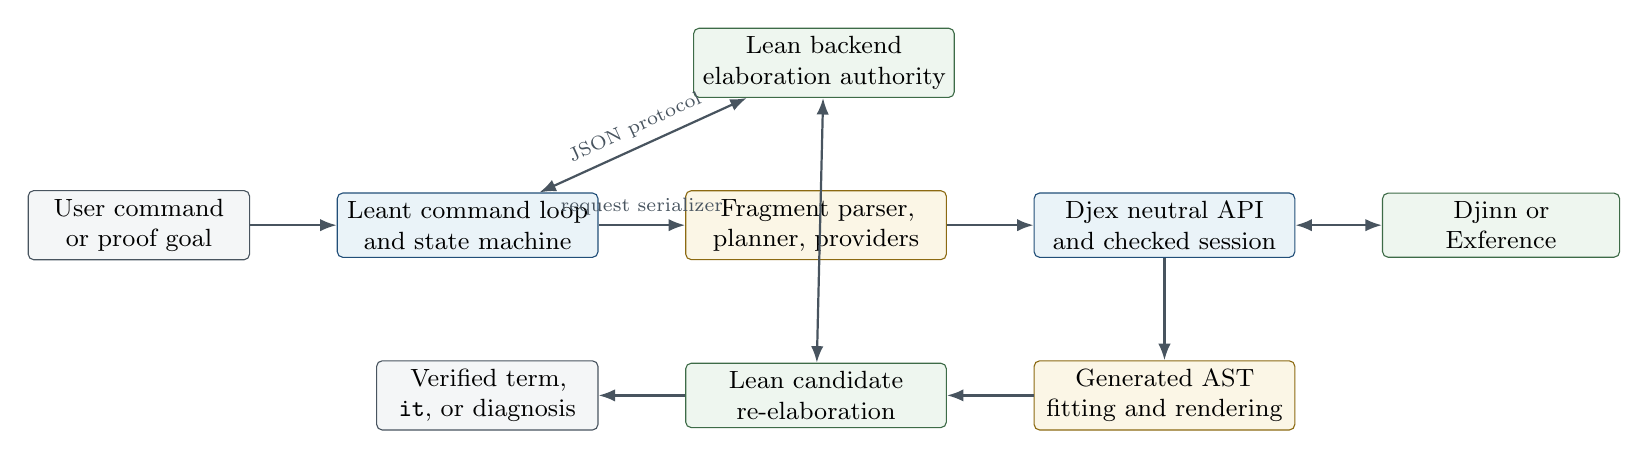
\begin{tikzpicture}[node distance=9mm and 11mm]
  \node[graybox,text width=26mm] (user) {User command\\or proof goal};
  \node[box,right=of user,text width=31mm] (leant) {Leant command loop\\and state machine};
  \node[greenbox,above right=12mm and 12mm of leant,text width=31mm] (lean) {Lean backend\\elaboration authority};
  \node[goldbox,right=of leant,text width=31mm] (frag) {Fragment parser,\\planner, providers};
  \node[box,right=of frag,text width=31mm] (djex) {Djex neutral API\\and checked session};
  \node[greenbox,right=of djex,text width=28mm] (engines) {Djinn or\\Exference};
  \node[goldbox,below=13mm of djex,text width=31mm] (render) {Generated AST\\fitting and rendering};
  \node[greenbox,left=of render,text width=31mm] (verify) {Lean candidate\\re-elaboration};
  \node[graybox,left=of verify,text width=26mm] (result) {Verified term,\\\code{it}, or diagnosis};

  \draw[flow] (user) -- (leant);
  \draw[flow] (leant) -- node[above,note]{request serializer} (frag);
  \draw[backflow] (leant) -- node[sloped,above,note]{JSON protocol} (lean);
  \draw[flow] (frag) -- (djex);
  \draw[backflow] (djex) -- (engines);
  \draw[flow] (djex) -- (render);
  \draw[flow] (render) -- (verify);
  \draw[backflow] (verify) -- (lean);
  \draw[flow] (verify) -- (result);
\end{tikzpicture}}
\caption{The runtime boundary. Lean and Djex are both authorities, but for different propositions. Djex validates and searches its own fragment; Lean decides whether the reconstructed source term actually inhabits the original Lean goal.}
\label{fig:joint-runtime}
\end{figure}

\section{The representation ladder}

A single successful \code{:synth} crosses at least six representations:

\begin{longtable}{@{}L{0.18\textwidth}L{0.27\textwidth}L{0.47\textwidth}@{}}
\toprule
\textbf{Representation} & \textbf{Owner} & \textbf{Purpose and information content} \\
\midrule
\endhead
Elaborated Lean expression & Lean backend & Full dependent expression, universes, implicit binders, reducible aliases, nominal constants, constructors, instances, and local context. This is the source truth. \\
Serialized fragment & Lean serializer in Leant's payload & A bounded S-expression describing only the structure Leant knows how to transport or analyze: arrows, products, sums, quantifiers, selected inductives, exact contexts, applications, atoms, and explicit incompleteness markers. \\
\code{Frag} value & Leant Haskell code & Parsed and analyzed bridge representation. It carries enough metadata to decide what search may inspect, what must remain opaque, how to render a candidate, and whether a negative result could be sound. \\
Djex neutral type and declarations & Shared Djex synthesis layer & Backend-independent Haskell type language, environment, class information, exact provider-instantiation evidence, query options, and generated-expression vocabulary. \\
Backend internal state & Djinn or Exference & Djinn uses formulas, sequents, proof terms, and structural plans. Exference uses typed holes, scopes, substitutions, a priority queue, constraints, and usage/rating metadata. \\
Shared generated AST & Djex & A checked neutral term language containing locals, globals, application, visible type application, tuples, lambdas, lets, cases, and patterns. It deliberately does not pretend to be Lean syntax. \\
Rendered Lean text & Leant & One or more source spellings after premise stripping, constructor restoration, binder uniquification, eta fitting, explicit-argument insertion, provider substitution, and idiomatic/fully explicit rendering. \\
Verified Lean term & Lean backend & The first spelling that elaborates against the exact original goal without an error, fatal response, or admitted proof. \\
\bottomrule
\end{longtable}

A recurring maintenance mistake is to collapse two adjacent rungs. For example, provider-instantiation evidence is semantic data used to justify a backend instantiation; provider-rendering metadata is source data used to reconstruct the right Lean spelling. They often describe the same occurrence, but they are not interchangeable.

\begin{invariantbox}
No stage is allowed to infer more certainty than the previous stage supplied. Opaque source structure may be transported, but it may not silently become decomposable. A bounded search may produce candidates, but exhaustion under a bound may not silently become a refutation. A pretty-printed type may guide diagnostics, but it may not silently become exact type evidence.
\end{invariantbox}

\section{Two independent axes: evidence and progress}

Both codebases take unusual care to keep \term{what the search established} separate from \term{why it stopped}. These are independent axes.

A search can finish and find candidates. It can finish and prove that the translated goal is uninhabited. It can finish without either kind of evidence because the backend is heuristic. It can be truncated after already finding candidates. It can also be truncated without finding a candidate, which is the weakest possible result. Djex therefore models progress with values such as \code{Finished} and \code{Truncated reason}, while modeling evidence separately. Leant then adds another filter: even a genuine Djex refutation may be unusable if the Lean-to-Djex projection hid relevant structure.

The practical consequence is a verdict lattice rather than a Boolean:

\begin{center}
\begin{tabularx}{0.94\textwidth}{@{}L{0.25\textwidth}L{0.28\textwidth}Y@{}}
\toprule
\textbf{Search observation} & \textbf{Safe user-level interpretation} & \textbf{Unsafe shortcut} \\
\midrule
Candidate and successful Lean check & The original Lean goal is inhabited by the checked term. & None; this is positive evidence at the final authority. \\
Djinn refutation, complete projection, no budget & The projected propositional goal is uninhabited; Leant may report a sound negative result. & Reporting it without checking fragment completeness. \\
Djinn no proof under budget & No candidate found within the budget. & Calling the goal uninhabited. \\
Exference queue exhausted & No candidate found by that heuristic search. & Treating queue exhaustion as a proof of impossibility. \\
Rendered candidate rejected by Lean & That spelling does not elaborate against the exact goal. & Concluding that the underlying semantic candidate is invalid; another spelling may work. \\
\bottomrule
\end{tabularx}
\end{center}

\section{The trust chain}

There are several checkers, and they prove different things:

\begin{enumerate}
  \item Djex smart constructors prove local representation invariants: names are valid, declarations are coherent, types are finite where required, queries are scoped, and exact assignment vectors satisfy widths and kinds.
  \item Djinn's proof checker proves that an LJT proof term derives the translated formula under the compiler's proof environment.
  \item Exference's expression checker reconstructs the candidate independently from search, using only the shared unification kernel and explicit provenance where necessary.
  \item Djex generated-syntax validation proves that the neutral term is structurally scoped and renderable in its own vocabulary.
  \item Lean elaboration proves the proposition users actually care about: the rendered term has the original Lean type in the original Lean environment.
\end{enumerate}

This is defense in depth, not redundancy. The internal checkers catch engine defects early and make Djex usable outside Lean. The final Lean check closes the semantic gap introduced by projection and source reconstruction.

\begin{sourcebox}
Start with the Djex architecture narrative in \dpath{docs/architecture.md}; the neutral facade in \dpath{src/Language/Haskell/Djex.hs}; Leant's process boundary in \lpath{src/Leant/Backend.hs}; and the top-level orchestration in \lpath{src/Main.hs}. The rest of this document decomposes those paths into maintainable subsystems.
\end{sourcebox}

\chapter{One synthesis request, end to end}\label{ch:end-to-end-overview}

This chapter gives a compact trace before the detailed subsystem chapters. Suppose the user asks Leant to synthesize a term for a goal morally equivalent to

\begin{lstlisting}[language=Leanish]
forall {a b : Sort u}, (a -> b) -> a -> b
\end{lstlisting}

The exact expression may contain universe levels, binder annotations, and local declarations. The bridge follows these stages.

\section{Stage 1: establish the exact Lean goal}

Leant determines the goal source. In ordinary mode this can be an explicit type or the type surrounding the most recent \code{sorry}. In prove mode it is the current target. Leant ensures that the derived synthesis environment corresponds to the current interactive environment; if declarations or imports changed, the synthesis base is rebuilt before any provider query is trusted.

Leant asks the Lean backend to execute a serializer payload. The payload runs after elaboration, so it examines \emph{expressions}, not surface text. It emits a bounded S-expression. The serializer records explicit versus implicit forall binders, instance/context information, the structural connectives it recognizes, and metadata for selected inductive occurrences. When it cannot safely descend, it emits an opaque or depth marker instead of guessing.

\section{Stage 2: parse and classify the fragment}

\code{Leant.Synth.Fragment} parses the S-expression into \code{Frag}. It then derives several views:

\begin{itemize}
  \item the leading binder spine, needed to align generated lambda binders with Lean's explicit, implicit, and instance slots;
  \item recursive-family keys, used to avoid importing irrelevant recursive constructor schemas;
  \item unsafe atoms and unsupported context markers, which may poison negative evidence but do not necessarily prevent positive synthesis;
  \item provider-query roots and result heads;
  \item a completeness summary for recursive and nominal projections;
  \item optional library premises serialized in the same batch.
\end{itemize}

For the example, the core fragment is a chain of foralls and arrows. Bound sort variables remain connected across the domains and codomain; they are not replaced with unrelated pretty-print names.

\section{Stage 3: choose search lanes}

Leant does not immediately dump every visible Lean declaration into one enormous search. It tries a staged policy:

\begin{enumerate}
  \item a structural, engine-only run;
  \item when enabled, a separately budgeted curated-library run;
  \item when the goal permits it, live-provider runs with gradually widening provider prefixes;
  \item optionally, a classical fallback for the precisely characterized quantifier-free fragment.
\end{enumerate}

The first stage is enough for the example because the target follows from its arguments alone. No provider discovery is needed.

\section{Stage 4: construct a checked Djex query}

\code{Leant.Synth.Engine} translates \code{Frag} into the shared Djex \code{Type}, creates any synthetic declarations and premises, constructs exact provider-instantiation assignments if providers are active, and builds a \code{QueryRequest}. The target name is a private synthetic definition such as \code{leantSynth}; the goal is the translated type; contexts are checked; backend options carry candidate, step, queue, and optional choice-point limits.

The backend adapter converts that public request into an opaque checked request associated with a validated session. This is where session-independent and session-dependent preflight occurs. A malformed request is rejected before search.

\section{Stage 5A: Djinn path}

Djinn compiles the translated type into an intuitionistic formula. For the example, after opening the positive universal prefix, the formula is essentially
\[
  (a \to b) \to a \to b.
\]
The LJT search introduces the two antecedents and applies the first to the second. It returns a proof term. The proof checker independently validates the derivation. The lowering pass converts the checked proof to the shared generated AST, approximately

\begin{lstlisting}[language=Haskellish]
Lambda [Bind "f", Bind "x"]
  (Apply (Local "f") (Local "x"))
\end{lstlisting}

The candidate stream carries positive evidence. Search progress records whether more candidates were omitted or a bound was reached.

\section{Stage 5B: Exference path}

Exference creates a root typed hole at the goal. Opening the forall prefix extends the rigid type scope. Introducing the arrows extends the term scope with \code{f} and \code{x}. To fill the result hole of type \code{b}, the search considers in-scope values and globals. Selecting \code{f : a -> b} creates an argument hole of type \code{a}; selecting \code{x : a} solves it. The resulting expression is simplified and then reconstructed by the independent expression checker.

Exference may rank several candidates and may stop due to step, depth, identifier, or queue limits. Even when its queue empties, it produces no proof of uninhabitability.

\section{Stage 6: fit and render}

Leant receives the neutral expression. The renderer strips synthetic premise binders, restores exact Lean global and constructor names, normalizes patterns into forms Lean accepts, uniquifies every binder, aligns lambda binders with the goal's explicit/implicit spine, inserts visible type placeholders where necessary, eta-expands selected forms, substitutes provider occurrences, and emits bounded source variants.

For the example, a likely first spelling is:

\begin{lstlisting}[language=Leanish]
fun f x => f x
\end{lstlisting}

A more explicit variant may also be retained when ambiguity exists. Variants are grouped because they represent one semantic candidate.

\section{Stage 7: ask Lean}

Leant sends a verification payload to the Lean backend. The payload checks each candidate against the exact original goal. A successful spelling is accepted; errors, fatal responses, and admitted terms are rejected. Verified candidates are displayed. Outside prove mode, Leant binds them as generated definitions in reverse quality order so the best surviving result becomes the newest bare \code{it}. In prove mode, it records proof splices that apply the candidate to the current hypotheses.

\begin{invariantbox}
A candidate only becomes a Leant result after the exact Lean backend accepts it. Djinn's proof and Exference's checker establish strong internal claims, but neither is allowed to substitute for final elaboration across the language boundary.
\end{invariantbox}

\part{Djex}

\chapter{Repository, package, and module map}\label{ch:djex-map}

\section{The package is one component with several source roots}

The top-level \dpath{djex.cabal} describes one package that deliberately preserves several historical trees while exposing a converged library. The important source roots are:

\begin{longtable}{@{}L{0.24\textwidth}L{0.68\textwidth}@{}}
\toprule
\textbf{Root} & \textbf{Responsibility} \\
\midrule
\endhead
\filepath{synthesis/src} & Shared synthesis vocabulary and validation: names, kinds, types, type atoms, constraints, declarations, environments, inventories, kind inference, queries, search progress, candidates, generated terms, diagnostics, selection, and rendering helpers. \\
\filepath{djinn/src-core} & Djinn's checked adapter, session/request internals, type-to-formula compiler, LJT proof search, proof checker, instantiation machinery, and proof-to-generated lowering. \\
\filepath{djinn/src-frontend} & Historical Djinn-compatible API and REPL facade. It is important for compatibility, but it should not own shared invariants. \\
\filepath{exference/src-core} & Exference's checked adapter and its engine: unification, class constraints, typed expression, typed holes, scopes, queue scheduler, scoring, rigid instantiation, independent expression checker, and diagnostics. \\
\filepath{exference/src-frontend} & Historical Exference source parser, environment loader, Haskell conversion layer, and CLI. \\
\filepath{src} & Unified Djex facade, unified command line and REPL, package/workspace handling, source translation, and the small public entry surface used by new clients. \\
\bottomrule
\end{longtable}

The Cabal file also exposes historical \code{djinn} and \code{exference} executables alongside \code{djex}. This is not merely packaging clutter. It lets the project maintain compatibility tests while moving semantic ownership into shared modules.

\begin{figure}[htbp]
\centering
\resizebox{0.97\textwidth}{!}{%
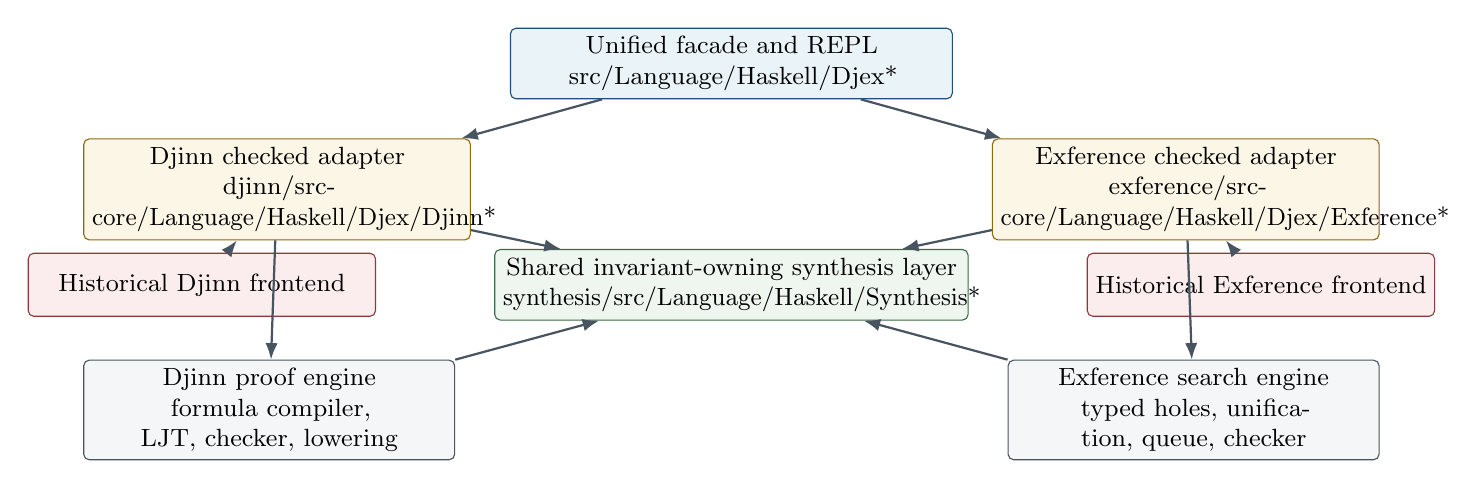
\begin{tikzpicture}[node distance=7mm]
  \node[box,text width=54mm] (facade) {Unified facade and REPL\\\filepath{src/Language/Haskell/Djex*}};
  \node[goldbox,below left=of facade,text width=47mm] (dadapter) {Djinn checked adapter\\\filepath{djinn/src-core/Language/Haskell/Djex/Djinn*}};
  \node[goldbox,below right=of facade,text width=47mm] (eadapter) {Exference checked adapter\\\filepath{exference/src-core/Language/Haskell/Djex/Exference*}};
  \node[greenbox,below=19mm of facade,text width=58mm] (shared) {Shared invariant-owning synthesis layer\\\filepath{synthesis/src/Language/Haskell/Synthesis*}};
  \node[graybox,below left=of shared,text width=45mm] (djinn) {Djinn proof engine\\formula compiler, LJT, checker, lowering};
  \node[graybox,below right=of shared,text width=45mm] (exf) {Exference search engine\\typed holes, unification, queue, checker};
  \node[redbox,left=15mm of shared,text width=42mm] (oldD) {Historical Djinn frontend};
  \node[redbox,right=15mm of shared,text width=42mm] (oldE) {Historical Exference frontend};

  \draw[flow] (facade) -- (dadapter);
  \draw[flow] (facade) -- (eadapter);
  \draw[flow] (dadapter) -- (shared);
  \draw[flow] (eadapter) -- (shared);
  \draw[flow] (dadapter) -- (djinn);
  \draw[flow] (eadapter) -- (exf);
  \draw[flow] (djinn) -- (shared);
  \draw[flow] (exf) -- (shared);
  \draw[flow] (oldD) -- (dadapter);
  \draw[flow] (oldE) -- (eadapter);
\end{tikzpicture}}
\caption{Djex's dependency intent. Shared semantic types sit below the adapters; backend-specific search remains sealed. The historical frontends point inward rather than defining new semantic authorities.}
\label{fig:djex-layers}
\end{figure}

\section{The central architectural rule}

The package converges infrastructure without pretending the engines are the same algorithm. Shared modules own contracts that both engines must honor. The adapters own conversion and backend policy. Djinn and Exference retain distinct search representations, ordering, completeness properties, and diagnostics.

This rule explains many otherwise surprising boundaries:

\begin{itemize}
  \item The shared \code{Type} is rich enough for both engines, but neither backend is forced to inspect every constructor identically.
  \item The shared \code{Generated} AST is a target language, but each backend may reach it by a different checked route.
  \item Search progress is shared, but the meaning of queue exhaustion differs from proof-search exhaustion.
  \item Provider-instantiation assignments are shared evidence, but each backend validates and consumes them in its own request preparation.
  \item The facade can expose a capability matrix instead of lying that every backend has every property.
\end{itemize}

\begin{designbox}
A tempting unification would be one giant \code{SearchState} and one generic step function parameterized by callbacks. That would erase exactly the information that makes the engines valuable: Djinn's proof-theoretic completeness story and Exference's ranking, type-directed expansion, and source-oriented heuristics. Djex instead unifies the borders and leaves the centers different.
\end{designbox}

\section{Recommended first reading order}

For a new maintainer, the shortest path to a correct mental model is:

\begin{enumerate}
  \item \dpath{synthesis/README.md} for the shared contract;
  \item \dpath{synthesis/src/Language/Haskell/Synthesis/Type.hs}, then \dpath{synthesis/src/Language/Haskell/Synthesis/Environment.hs};
  \item \dpath{synthesis/src/Language/Haskell/Synthesis/Query.hs}, \dpath{synthesis/src/Language/Haskell/Synthesis/Search.hs}, and \dpath{synthesis/src/Language/Haskell/Synthesis/Generated.hs};
  \item \dpath{djinn/src-core/Language/Haskell/Djex/Djinn.hs} and \dpath{djinn/src-core/Djinn/Core.hs};
  \item \dpath{exference/src-core/Language/Haskell/Djex/Exference.hs} and \dpath{exference/src-core/Language/Haskell/Exference/Core/Internal/Exference.hs};
  \item \dpath{src/Language/Haskell/Djex.hs} and the unified REPL modules.
\end{enumerate}

Do not start by reading the two largest backend files linearly. First learn what their inputs and outputs are permitted to mean. Otherwise implementation details such as freshness supplies, proof-plan families, or queue pruning have no frame of reference.

\chapter{The shared synthesis foundation}\label{ch:djex-shared}

\section{Names are checked data, not strings}

The shared name layer in \dpath{synthesis/src/Language/Haskell/Synthesis/Name.hs} distinguishes namespaces and syntactic roles. Values such as identifiers, type constructor names, data constructor names, class names, method names, and definition names are not freely interchangeable. Smart constructors validate spellings and reserved forms; rendering can therefore rely on the distinction without reparsing arbitrary text.

This is a small example of the project's general style: validate once, hide the constructor, and pass an authority value downward. A backend should not have to ask repeatedly whether the query target is a legal definition name.

The layer also separates semantic identity from qualification and source spelling. That matters because a generated term may need a fully qualified source name even though environment lookup used a canonical key, and because a local binder must never be confused with a global declaration merely because the text matches.

\section{Kinds and the neutral type language}

The neutral type language is centered in \dpath{synthesis/src/Language/Haskell/Synthesis/Type.hs}. At a high level it contains:

\begin{lstlisting}[language=Haskellish]
data Variable id
  = FlexibleVariable id
  | RigidVariable id

data Type v
  = TypeVariable v
  | TypeConstructor Name
  | TypeApplication (Type v) (Type v)
  | FunctionType (Type v) (Type v)
  | TupleType Boxity [Type v]
  | ForallType [v] [Constraint (Type v)] (Type v)
\end{lstlisting}

The precise exported surface is richer, but this sketch captures the semantic split. Flexible variables are unification variables in Exference and instantiation variables in shared validation. Rigid variables are constants scoped by a binder or exact assignment. A forall stores its binders and class constraints explicitly. Tuples retain boxity and arity rather than being flattened to anonymous constructor applications at the public boundary.

\subsection{Canonical forms without erasing source distinctions}

The module provides canonical function and tuple views, strict application and function spines, constructor-application views for higher-kinded unification, free-variable and binder analysis, global binder renaming, and capture-avoiding simultaneous substitution.

The important qualification is \emph{without erasing source distinctions}. Normalization may turn a saturated representation into a canonical form for comparison, but it must not dissolve a nested polytype into ordinary first-order nodes or forget that a nominal constructor came from a particular source declaration.

For example, higher-kinded unification wants to observe
\[
  F\;a\;b
\]
as a head plus arguments, and it wants functions and tuples to participate in the same application machinery. That is the purpose of a constructor-application view. It is not permission to rewrite every type permanently into an untyped list of symbols.

\subsection{Finite observation boundaries}

Many public values are Haskell lists, and clients can accidentally supply cyclic or infinite lists. Constructors that must establish a finite invariant do not blindly call \code{length}. They observe only a documented maximum width plus a sentinel element, then reject oversize or nonterminating shapes at a bounded frontier where possible. The same principle appears in provider assignment vectors, class arities, kind trees, generated hints, and search prefixes.

\begin{invariantbox}
Strict authorities never retain a value whose validity depends on consuming an unbounded lazy tail. Laziness is reserved for search result streams and other places where incremental observation is itself the API.
\end{invariantbox}

\section{Type atoms: opaque, alpha-aware islands}

\dpath{synthesis/src/Language/Haskell/Synthesis/TypeAtom.hs} solves a particularly difficult problem. A nested polymorphic type can be meaningful as a whole without being safe to decompose in a first-order unifier. Djex therefore represents such a region as a \code{TypeAtom}: an exact source tree paired with an alpha-normal lexical key and enough variable information for substitution and occurs checks.

Ordinary unification treats the atom as opaque. Equality remains alpha-aware. Free variables inside the atom still participate in capture avoidance and occurs checks. Thus Djex avoids two unsound extremes:

\begin{itemize}
  \item treating the atom as a completely uninterpreted string, which would lose alpha-equivalence and variable provenance;
  \item opening the atom as if rank-N structure were ordinary first-order syntax, which would allow invalid decomposition and escaping binders.
\end{itemize}

Type atoms recur in both backends. Djinn may compile a nested negative forall to an opaque proposition symbol keyed by a type atom. Exference's unifier may bind an opaque polytype as one unit but cannot descend into it.

\section{Constraints, classes, declarations, and synonyms}

The shared declaration vocabulary spans \dpath{synthesis/src/Language/Haskell/Synthesis/Constraint.hs}, \dpath{synthesis/src/Language/Haskell/Synthesis/Class.hs}, \dpath{synthesis/src/Language/Haskell/Synthesis/Declaration.hs}, and \dpath{synthesis/src/Language/Haskell/Synthesis/TypeSynonym.hs}. It models value signatures, data/type declarations, classes, instances, methods, constraints, and type synonyms in source order.

Source order is significant. A declaration can only refer to authorities already established by the prefix unless a specific recursive form permits otherwise. Type-synonym expansion must terminate or report a cycle. Class validation must know arity, superclass prerequisites, method ownership, and instance-head shape. Those checks belong before either backend builds a session.

The shared kind inference module, \dpath{synthesis/src/Language/Haskell/Synthesis/KindInference.hs}, validates type applications and exact provider assignments across proper and higher kinds. This is why provider evidence carries kind information rather than a flat list of types.

\section{Environment as an authority}\label{sec:djex-environment}

\dpath{synthesis/src/Language/Haskell/Synthesis/Environment.hs} is one of the most important files in the repository. The public \code{Environment} is opaque. Internally it retains the source declarations and several strict indexes: types, values, constructors, classes, instances, instance heads, and occupied names. \code{mkEnvironment} validates the entire declaration sequence before constructing those indexes.

The indexes are duplicated views of one semantic state. An update must therefore be transactional: either the declaration and all relevant indexes advance together, or the old environment remains. Code that appends a declaration to the source list but forgets an instance-head index would create an internally contradictory authority.

A useful way to read the constructor is as a fold over declarations with a large invariant:

\begin{lstlisting}[language=Haskellish]
step :: CheckedPrefix -> Declaration -> Either Diagnostic CheckedPrefix
step prefix declaration = do
  validateNamespaces prefix declaration
  validateKinds      prefix declaration
  validateClasses    prefix declaration
  validateInstances  prefix declaration
  updateEveryIndex   prefix declaration
\end{lstlisting}

This is explanatory pseudocode, not a literal excerpt. The actual code has more specialized paths, but the transactional model is accurate.

\subsection{Inventory and prepared inventory}

\dpath{synthesis/src/Language/Haskell/Synthesis/Inventory.hs} derives a search-oriented inventory from the environment. A prepared inventory is another opaque authority: aliases are expanded where permitted, recursive components are classified, and lookup tables are normalized for backend consumption.

The project also distinguishes a transient \emph{prepared-inventory expansion}. That view may expose alias-free structures and recursion metadata for a particular operation, but it is not retained as a long-lived authority. This prevents a temporary expansion policy from silently becoming the canonical meaning of the environment.

\begin{designbox}
The environment answers, ``What declarations exist and are they coherent?'' The inventory answers, ``What search-facing facts can be derived from that environment?'' A prepared expansion answers, ``What does this particular type look like after this bounded expansion policy?'' Keeping these questions in separate types prevents a backend convenience from mutating source semantics.
\end{designbox}

\section{Queries and checked requests}

The public query language in \dpath{synthesis/src/Language/Haskell/Synthesis/Query.hs} contains a target definition name, a goal type, explicit contexts, and backend options. Provenance and display metadata may accompany the query, but semantic equality does not accidentally depend on incidental diagnostics.

A \code{CachedQuery} is opaque. It represents the result of normalization and validation that can safely be reused. The backend adapters then add session-specific checks and wrap it in private \code{DjinnRequest} or \code{ExferenceRequest} types. This two-stage preparation has a practical payoff: malformed shape is rejected once, while environment-dependent facts are checked against the exact session that will execute the query.

Provider evidence is part of the request contract. The shared forms distinguish:

\begin{itemize}
  \item a provider-instantiation candidate, describing a possible relation between a provider and a query occurrence;
  \item an assignment, choosing concrete arguments for that provider;
  \item a kinded assignment, retaining each argument's kind and exact representation.
\end{itemize}

The vectors are bounded. At this snapshot, a provider assignment supports at most six arguments, with finite caps on candidates and assignments. These limits are not merely performance knobs; they are part of the validation boundary that keeps exact evidence inspectable.

\section{Search progress and evidence}

\dpath{synthesis/src/Language/Haskell/Synthesis/Search.hs} defines backend-neutral progress. Truncation reasons include step and choice-point limits, candidate cutoffs, identifier exhaustion, queue pruning, and depth pruning. A batch can be continuing or completed; completion can be finished or truncated with one or more exact reasons.

The evidence layer remains backend-specific enough to be honest. Djinn can return validated candidates, a proof of uninhabitability for the translated problem, a self-reference-only diagnosis, or no evidence. Exference returns candidates and progress but never manufactures a negative proof from heuristic exhaustion.

\subsection{Candidate values}

\dpath{synthesis/src/Language/Haskell/Synthesis/Candidate.hs} packages a generated function clause with residual constraints and backend details. Backend details are intentionally extensible: Djinn can report proof/search information, while Exference can report steps, queue size, penalty, usage, and pruning statistics.

Candidate rendering revalidates scope. This may seem late, but it is a deliberate last defense before a neutral term crosses into source syntax. A candidate with an unbound local or an unresolved hole is not made printable merely because the search happened to construct it.

\section{The generated-term language}\label{sec:generated-ast}

The large \dpath{synthesis/src/Language/Haskell/Synthesis/Generated.hs} module is the common target of both backends. Its expression vocabulary includes locals, globals, holes during construction, application, visible type application, tuples, lambdas, lets, and cases. Patterns include binders, wildcards, tuples, declared constructors, and as-patterns. Function clauses associate checked definition names with expressions.

Several details are easy to miss:

\begin{itemize}
  \item \term{Visible type application} is a real AST node. It is not a string annotation. This lets exact rank-N instantiation evidence survive into rendering.
  \item Application-spine helpers are strict about mixed term and type arguments. They preserve order and do not silently commute them.
  \item Scope validation understands every binder-introducing pattern, including nested tuple and constructor patterns.
  \item Simplification is capture-aware and must preserve the source of global versus local names.
  \item Qualification is postponed until rendering, so semantic identity and source spelling remain separate.
\end{itemize}

\begin{invariantbox}
The shared generated AST is neither Haskell source nor Lean source. It is a checked intermediate language. Backend code may construct it; frontend code may render it; neither side may attach semantics by concatenating unvalidated strings.
\end{invariantbox}

\section{Diagnostics and selection}

\dpath{synthesis/src/Language/Haskell/Synthesis/Diagnostic.hs} gives validation and search failures structured identities and renderings. The adapters use diagnostics instead of throwing ordinary exceptions for expected user errors. Pure rendering paths still contain exception boundaries around hostile or infinite user-supplied text, but asynchronous exceptions are preserved.

\dpath{synthesis/src/Language/Haskell/Synthesis/Selection.hs} separates search generation from candidate selection. A backend may expose a lazy stream with scores and progress; a client chooses a bounded subset, filters it, and preserves the strongest progress observation. This is particularly important for Leant, which performs its own cross-engine merge and final verification window.

\begin{summarybox}
The shared layer establishes the vocabulary and the facts that both engines are allowed to assume. Its most important contribution is not code reuse but semantic compression: downstream code receives opaque values that stand for completed validation arguments.
\end{summarybox}

\chapter{Djinn: formulas, LJT proof search, and checked lowering}\label{ch:djinn}

\section{What Djinn promises}

Djinn is the proof-theoretic backend. It translates a supported type problem into intuitionistic propositional logic, searches for proof terms in a contraction-free LJT-style calculus, checks every proof independently, and lowers accepted proofs into the shared generated syntax. When translation is complete and search is genuinely exhaustive, failure can be negative evidence. That last property is the reason Djinn's request preparation, translation plans, and progress accounting are more elaborate than a simple ``type to formula'' function.

The stable adapter is \dpath{djinn/src-core/Language/Haskell/Djex/Djinn.hs}. Its private request and session support live in \dpath{djinn/src-core/Language/Haskell/Djex/Djinn/Internal/Request.hs} and \dpath{djinn/src-core/Language/Haskell/Djex/Djinn/Internal/Session.hs}. The major engine entry points are in \dpath{djinn/src-core/Djinn/Core.hs}.

\section{Request preparation}

Preparation occurs in two layers.

\subsection{Session-independent preflight}

The adapter first validates facts that do not depend on a loaded environment: the target definition name, goal width, binder shape, explicit context width, option bounds, and finite observations. This stage turns a public \code{QueryRequest} into a normalized cached query or a structured diagnostic.

The benefit is deterministic failure. A malformed query should not fail differently depending on which session happened to receive it, nor should it force a large environment before reporting a simple width error.

\subsection{Session-dependent elaboration}

The checked session supplies declarations, classes, constructor inventories, kind information, synonyms, and source names. The private request builder:

\begin{itemize}
  \item resolves and normalizes the goal against the prepared inventory;
  \item checks explicit class contexts against declared class arities;
  \item embeds contexts under the leading forall prefix in a representation that preserves scope;
  \item makes binder implicitness explicit to the compiler;
  \item verifies exact provider-instantiation assignments against the session;
  \item determines which loaded values and constructor schemas are eligible premises;
  \item excludes the target from the ordinary premise set.
\end{itemize}

Explicit contexts are validation obligations, not ordinary proof assumptions. A request for \code{C a => a -> a} should not be solved by treating the class dictionary as an arbitrary value of proposition \code{C a}; its role is to constrain the type and the admissible instances.

\begin{pitfallbox}
Reintroducing the target definition as a normal premise makes every recursive query trivially inhabitable. Djinn excludes it from the safe search environment. A separate diagnostic lane may reintroduce it only to establish that all observed proofs require self-reference.
\end{pitfallbox}

\section{The logical language}

\dpath{djinn/src-core/Djinn/Internal/LJTFormula.hs} defines the formula and proof-term vocabulary. In simplified form:

\begin{lstlisting}[language=Haskellish]
data Formula
  = Conj [Formula]
  | Disj [(ConsDesc, Formula)]
  | Empty Symbol
  | Formula :-> Formula
  | PVar Symbol

data Term
  = Var ... | Lam ... | Apply ...
  | Ctuple ... | Csplit ...
  | Cinj ... | Ccases ... | Xsel ...
\end{lstlisting}

Products become conjunctions; algebraic alternatives become labeled disjunctions; functions become implication; empty nominal types and opaque atoms become symbols. Constructor descriptions retain enough information for proof lowering to recover data-constructor applications and case alternatives.

\subsection{Symbols preserve nominal and opaque identity}

A symbol can be an ordinary logical name or an opaque type symbol paired with source information and a \code{TypeAtomKey}. This prevents two unrelated empty nominal types from collapsing merely because each has no visible constructor. It also ensures that alpha-equivalent opaque polytypes compare correctly while distinct nested polytypes remain distinct.

This is essential for sound negative evidence. If the compiler identified all opaque regions with one proposition, it could invent implications between unrelated source types. If it generated a fresh proposition for each occurrence, it would lose valid forwarding of the same opaque type. The key must therefore be semantic and alpha-aware.

\section{The prepared formula compiler}\label{sec:djinn-compiler}

\dpath{djinn/src-core/Djinn/Internal/TypeFormula.hs} is the bridge between the shared type authority and the proof calculus. It is best understood as a compiler producing both code and a proof obligation ledger.

A prepared compiler caches validated definitions, constructor descriptions, synonym expansions, and recursive-component classifications. A translation result contains at least:

\begin{itemize}
  \item the formula;
  \item whether the translation was incomplete;
  \item which positive forall sites were opened;
  \item which binders were skolemized;
  \item occurrence and origin metadata used to validate exact provider assignments;
  \item enough nominal information to lower a proof back to generated syntax.
\end{itemize}

\subsection{One-layer views}

The compiler does not recursively destruct every type by default. It uses a one-layer \code{TypeView}: observe the current constructor, decide whether that constructor is structurally admissible in the current polarity, and recursively compile only the selected children. This makes polarity and opacity policy explicit.

\subsection{Forall polarity}

A positive forall corresponds to producing a polymorphic value. Djinn can often open it by introducing a fresh rigid symbol. A negative forall corresponds to consuming a polymorphic value. Naively opening it would require impredicative or higher-rank reasoning beyond ordinary propositional translation. The conservative default is therefore:

\begin{itemize}
  \item open selected positive forall sites;
  \item preserve negative and unsupported nested sites as opaque type atoms;
  \item add exact instantiation axioms only when the request carries checked evidence.
\end{itemize}

This is why rank-N support appears as a family of translation plans rather than a single recursive function.

\subsection{Bounded plan families}

For a query with several openable sites, the compiler explores a deterministic family of structural plans:

\begin{itemize}
  \item all sites open;
  \item all sites opaque;
  \item selected singleton, pair, triple, quadruple, and quintuple frontiers in both open and opaque orientations;
  \item additional guarded plans tied to exact provider assignments and query-correlated closed instantiations.
\end{itemize}

The family is explicitly bounded. Quintuple combinations are capped per orientation, while remaining complete through a documented small number of sites. The cap is not hidden: if relevant plans were omitted, the translation carries incompleteness and a candidate-free search cannot become a refutation.

\begin{designbox}
Opening every positive forall is not always best. An opened site exposes structure that can enable a proof, but it can also destroy useful opaque equality: a value may simply need to be forwarded unchanged. The plan family searches both interpretations and deduplicates equivalent results afterward.
\end{designbox}

\subsection{Recursive and nominal data}

Recursive types require a similar duality. At a positive occurrence, the compiler may expose one constructor layer to synthesize or inspect data. At the same time it preserves an exact opaque fallback so forwarding remains possible without infinite unfolding. Recursive components are classified before compilation, and every exposure decision contributes to the completeness ledger.

Nominal parametric data is transported with constructor descriptions and parameter metadata. The compiler must not substitute a structurally similar but differently named type. Exact constructor identity is carried into proof terms and later lowering.

\subsection{Exact provider-assignment retention}

Provider assignments are only useful if the formula still represents the exact argument vector that was validated at the source boundary. The compiler records origins and occurrence paths and checks that a structural plan retains the assignment across aliases and higher-kinded application. A plan that has hidden or rearranged a relevant argument cannot consume the assignment merely because its pretty-printed formula looks compatible.

\section{LJT search}\label{sec:ljt-search}

The proof search implementation is in \dpath{djinn/src-core/Djinn/Internal/LJT.hs}. It combines a contraction-free sequent calculus with a continuation-encoded lazy search monad.

\subsection{Search modes}

A search mode chooses an exploration strategy and an optional global choice-point budget. The principal strategies are depth-first exploration and fair interleaving. The default unbudgeted mode is intended to retain the calculus's completeness properties, subject to documented local fairness adjustments.

The result stream is lazy. A client may consume the first proof without constructing every proof. At the same time, budget and exhaustion information remain observable. Internally, the search distinguishes:

\begin{itemize}
  \item a completed branch;
  \item a yielded proof with a continuation;
  \item an administrative step that advances the proof machine without producing a proof.
\end{itemize}

This distinction permits exact choice-point accounting and fair merges without forcing the whole tree.

\subsection{Antecedent classification}

LJT gains much of its behavior by classifying antecedents. The implementation separates pending formulas, atomic implications, nested implications, and already available atomic proofs. Right-reduction introduces functions, products, or disjunction choices. Left-reduction selects an assumption and applies the appropriate elimination rule.

The calculus is contraction-free in its structural formulation: it avoids arbitrary duplication as a primitive rule. Where a proof term must use an assumption more than once, the formula-specific left rule accounts for it. This keeps the search space much smaller than a naive natural-deduction enumerator.

\subsection{Cheap reachability pruning}

A necessary-condition test, conceptually \code{goalMayBeReachable}, rejects branches whose atomic goal symbols cannot arise from the current antecedents. This is not a theorem prover by itself; it is a conservative prune. Returning false must mean the branch is impossible. Returning true merely allows full proof search to continue.

\subsection{Fairness for repeated endomorphisms}

Types with several endomorphism assumptions can produce infinite local families such as \code{f x}, \code{f (f x)}, and so on. Pure depth-first exploration can starve sibling compositions. The implementation applies a local round-robin or interleaving policy for repeated binary endomorphism opportunities. Freshness and substitution machinery ensure that copied proof fragments do not capture binders.

\subsection{Normalization}

Proof terms are normalized before checking and lowering. The normalizer beta-reduces lambda applications, tuple split redexes, and case/injection redexes. Normalization reduces duplicate candidates and gives the proof checker a simpler object. It must remain binder-safe: every copied binder is freshened before substitution.

\begin{figure}[htbp]
\centering
\resizebox{0.96\textwidth}{!}{%
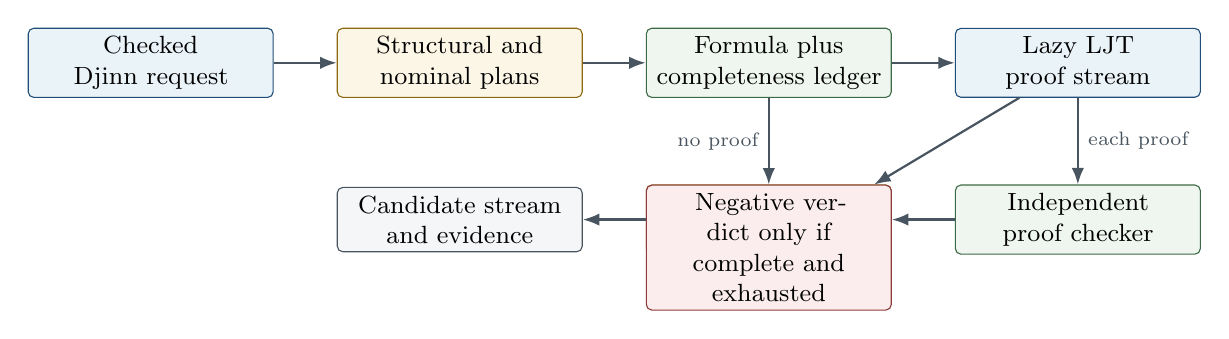
\begin{tikzpicture}[node distance=8mm and 8mm]
  \node[box] (request) {Checked\\Djinn request};
  \node[goldbox,right=of request] (plans) {Structural and\\nominal plans};
  \node[greenbox,right=of plans] (formula) {Formula plus\\completeness ledger};
  \node[box,right=of formula] (ljt) {Lazy LJT\\proof stream};
  \node[greenbox,below=11mm of ljt] (check) {Independent\\proof checker};
  \node[goldbox,left=of check] (lower) {Proof-to-generated\\lowering};
  \node[graybox,left=of lower] (candidate) {Candidate stream\\and evidence};
  \node[redbox,below=11mm of formula] (negative) {Negative verdict only if\\complete and exhausted};

  \draw[flow] (request) -- (plans);
  \draw[flow] (plans) -- (formula);
  \draw[flow] (formula) -- (ljt);
  \draw[flow] (ljt) -- node[right,note]{each proof} (check);
  \draw[flow] (check) -- (lower);
  \draw[flow] (lower) -- (candidate);
  \draw[flow] (formula) -- node[left,note]{no proof} (negative);
  \draw[flow] (ljt) -- (negative);
\end{tikzpicture}}
\caption{Djinn's proof-producing pipeline. The negative edge is guarded by both compiler completeness and search exhaustion.}
\label{fig:djinn-pipeline}
\end{figure}

\section{Core orchestration and instantiation axioms}

\dpath{djinn/src-core/Djinn/Core.hs} orchestrates plan construction, premise selection, LJT execution, proof validation, deduplication, ranking, and evidence. The file is large because it is where independent correctness conditions meet.

The engine can derive several classes of controlled instantiation premise:

\begin{itemize}
  \item closed monotype instantiations available from the query itself;
  \item query-correlated instantiations whose shared variables must receive one coherent assignment;
  \item loaded polymorphic values whose exact schemes are known in the session;
  \item provider-local assignments supplied by Leant or another client;
  \item visible type-application evidence retained in the generated term.
\end{itemize}

These are not unconstrained axioms. Each is created from a checked source scheme, exact argument vector, kind proof, and plan-retention check. After the proof checker validates a derivation in the enriched proof environment, the instantiation evidence is rewritten or erased in a controlled lowering step so the generated term refers to actual source values and visible type applications rather than fictional logical constants.

\section{Proof checking and lowering}

Every LJT proof is passed to \dpath{djinn/src-core/Djinn/Internal/ProofCheck.hs}. The checker reconstructs the derivation against the formula and proof environment. Search ordering, cached reachability, and heuristic plan choice are not trusted as proof evidence.

Accepted proofs are converted by \dpath{djinn/src-core/Djinn/Internal/ProofToGenerated.hs}. The lowering pass maps logical introductions and eliminations to lambda, application, tuple, constructor, and case syntax; restores source constructor identities; resolves instantiation witnesses; and produces a shared generated clause. Scope is checked again at the shared AST boundary.

\begin{invariantbox}
Djinn's trusted result is not ``the search code said success.'' It is ``the independent checker accepted this proof term for this translated formula, and the lowering pass produced a scoped generated term.'' The final client may still need to check that translation and rendering preserve the source-language goal.
\end{invariantbox}

\section{Evidence outcomes}

Conceptually, the core can distinguish:

\begin{itemize}
  \item \term{realized}: one or more checked candidates exist;
  \item \term{unrealizable}: exhaustive complete search found no proof;
  \item \term{unrealizable without self-reference}: a diagnostic run proves that only reintroducing the target enables a proof;
  \item \term{undecided}: a budget, incomplete plan family, opaque unsupported structure, or other limitation prevents a verdict.
\end{itemize}

A global candidate cutoff is shared across plans. To know whether the cutoff actually truncated a nonempty tail, the implementation observes one extra proof as a witness. Choice-point budgets are likewise shared across plan execution rather than reset per plan. Otherwise a caller requesting a budget of \(N\) could accidentally receive \(N\) work for every structural plan.

Candidates from different plans are deduplicated after normalization, including structural and eta-equivalent forms where the shared representation can establish equivalence. Optional ranking favors compact terms and can consider unused-binder ratios.

\section{Worked trace: identity}

For \code{forall a. a -> a}, a representative trace is:

\begin{enumerate}
  \item Request preparation validates one leading forall and no class context.
  \item A positive-forall plan opens \code{a} as a fresh rigid proposition symbol.
  \item The compiler emits \(a \to a\).
  \item Right implication introduction extends the antecedent with \(x:a\) and sets goal \(a\).
  \item The atomic goal is discharged from the antecedent, yielding a variable proof.
  \item The proof is wrapped in a lambda, normalized, and checked.
  \item Lowering emits a lambda over one local binder.
  \item The plan family may also consider an opaque interpretation, but deduplication removes equivalent forwarding terms.
\end{enumerate}

The apparent triviality is misleading. The same machinery must retain alpha identity if the forall is nested, avoid opening it at a negative polarity without evidence, and keep the binder rigid in the proof environment.

\section{Worked trace: swapping a product}

For \code{(a,b) -> (b,a)}, the compiler emits a conjunction implication. Search introduces the input, splits it into two components, constructs a conjunction in reverse order, and returns a proof term using tuple split and tuple construction. Lowering chooses a generated pattern/case representation. Later frontends may render it as a tuple-pattern lambda or as an explicit match depending on target-language constraints.

This trace is a useful debugging probe because it crosses both an elimination and an introduction, exercises binder scopes created by a destructuring pattern, and reveals whether normalization preserves constructor descriptions.

\section{Debugging Djinn}

When Djinn unexpectedly returns no term, inspect in this order:

\begin{enumerate}
  \item Was the public query rejected or was a checked request actually constructed?
  \item Which type regions became opaque, and did the compiler mark translation incomplete?
  \item Which structural plans were generated and which exact assignments survived each plan?
  \item Were relevant loaded values or constructors omitted by premise policy?
  \item Did the LJT stream exhaust, hit a choice-point budget, or hit the candidate cutoff?
  \item Did a proof appear but fail \code{ProofCheck}?
  \item Did lowering or generated-scope validation reject it?
  \item Did client-side rendering or final source elaboration reject the neutral candidate?
\end{enumerate}

The distinction between steps 5, 6, and 8 is particularly important. A proof-search defect, a proof-checker rejection, and a Lean elaboration rejection require entirely different fixes.

\begin{sourcebox}
The shortest source trail through a Djinn request is: \dpath{djinn/src-core/Language/Haskell/Djex/Djinn.hs} $\rightarrow$ \dpath{djinn/src-core/Language/Haskell/Djex/Djinn/Internal/Request.hs} $\rightarrow$ \dpath{djinn/src-core/Djinn/Core.hs} $\rightarrow$ \dpath{djinn/src-core/Djinn/Internal/TypeFormula.hs} $\rightarrow$ \dpath{djinn/src-core/Djinn/Internal/LJT.hs} $\rightarrow$ \dpath{djinn/src-core/Djinn/Internal/ProofCheck.hs} $\rightarrow$ \dpath{djinn/src-core/Djinn/Internal/ProofToGenerated.hs}.
\end{sourcebox}

\chapter{Exference: typed-hole search, ranking, and reconstruction}\label{ch:exference}

\section{What Exference promises}

Exference is the heuristic and ranking-oriented backend. It searches a state space of partially constructed typed expressions. Nodes contain typed holes, lexical scopes, rigid and flexible type variables, class obligations, globals, exact provider evidence, constructor/deconstructor knowledge, usage counts, freshness supplies, and a priority score. The scheduler expands the most promising node, bounds the queue and depth, and emits solved expressions. An independent checker reconstructs each candidate before it crosses the adapter boundary.

Exference is often better than Djinn when a useful term should call a library value, when several plausible terms need ranking, or when rank-N elimination and explicit type applications are involved. Its negative result is intentionally weaker: it does not claim that queue exhaustion proves uninhabitability.

The adapter starts at \dpath{exference/src-core/Language/Haskell/Djex/Exference.hs}; the central scheduler is \dpath{exference/src-core/Language/Haskell/Exference/Core/Internal/Exference.hs}; node data and construction are in \dpath{exference/src-core/Language/Haskell/Exference/Core/Internal/ExferenceNode.hs} and \dpath{exference/src-core/Language/Haskell/Exference/Core/Internal/ExferenceNodeBuilder.hs}.

\section{Checked environment and request}

The adapter builds an opaque Exference session from the shared environment. It projects declarations, class information, constructor/deconstructor bindings, ratings, visibility, and prepared schemes into Exference-specific authorities. Projection can omit unsupported declarations, but omissions are returned as diagnostics rather than silently changing the query.

A checked Exference query seals together:

\begin{itemize}
  \item the exact prepared environment;
  \item the normalized goal and explicit contexts;
  \item global and local source-name mappings;
  \item provider candidates and exact assignments;
  \item a rigid-instantiation plan;
  \item search options and penalty overrides.
\end{itemize}

Assignment validation checks exact provider scheme identity, argument count, absence or treatment of contexts, kinds, closure, finite widths, and duplicates. A textual name match is insufficient.

\section{Types and unification}\label{sec:exference-unify}

The core reuses the shared neutral type through compatibility patterns. \dpath{exference/src-core/Language/Haskell/Exference/Core/Types.hs} defines Exference-facing views, substitutions, polytype helpers, and scope-sensitive operations. The actual unifier is \dpath{exference/src-core/Language/Haskell/Exference/Core/Unify.hs}.

\subsection{Disjoint and shared namespaces}

Exference needs several unification modes. Two schemes may use the same integer identifiers but mean different variables; a local expression and a global scheme may share a rigid scope; a right-hand pattern may contain the only variables permitted to bind. The API therefore distinguishes disjoint, shared, and one-sided unification rather than relying on caller folklore.

Internally, variables are tagged with their origin before unification. This prevents accidental capture or identification merely because two integer supplies both started at zero.

\subsection{Higher-kinded heads}

The unifier observes a constructor-application form. Functions and tuples can be lowered to canonical heads for this purpose, so a flexible head variable can bind to a type constructor of the right kind. Kind checking is not deferred until rendering: a substitution that solves the first-order shape but violates kind arity is rejected.

\subsection{Opaque polytypes}

Nested polytypes become tagged opaque atoms. They can unify as complete values when their alpha-normal keys and substitutions agree, but the unifier cannot decompose a forall under an application as if it were a monotype. Occurs checks still inspect the atom's free variables. Substitution into the atom is capture-avoiding.

\begin{invariantbox}
A nested forall is simultaneously opaque to structural decomposition and transparent to lexical hygiene. ``Opaque'' never means ``free-variable blind.''
\end{invariantbox}

\section{Classes and residual constraints}

Exference builds a static class environment from validated class and instance declarations. It checks duplicate or overlapping instance heads according to the supported policy, class arity, superclass cycles, and recursively expanding prerequisites. Search may carry scoped givens and unresolved obligations. A solved expression is only a candidate after constraint closure determines which residual constraints are valid and whether they escape the permitted scope.

The expression checker later recomputes residual constraints and compares them with the candidate's claimed set. Search cannot simply attach a convenient list.

\section{The search node}\label{sec:exference-node}

A node is a complete snapshot of one partial program. Important fields include:

\begin{itemize}
  \item pending typed holes and the already selected next goal;
  \item a scope forest describing lexical parentage;
  \item local givens and scoped class constraints;
  \item flexible substitutions and rigid scopes;
  \item global bindings with exact schemes and source identities;
  \item visible type-application candidates;
  \item provider candidate and assignment maps;
  \item constructor and deconstructor bindings;
  \item per-binding usage counts and donation guards;
  \item the current annotated generated expression;
  \item fresh supplies for term variables, type variables, scopes, and holes;
  \item accumulated depth, last selected binding, and score inputs.
\end{itemize}

The apparent duplication is deliberate. Search branches must be clonable and self-describing. A node should not depend on mutable ambient state whose meaning changes after it is enqueued.

\subsection{Typed goals}

A pending goal records a hole identifier, expected type, lexical scope, forall-introduction mode, tuple policy, and local givens. Forall goals can be in phases such as opening an existing leading prefix, trying an introduction, or continuing a previously selected introduction. Tuple goals can choose a shallow structural lane or a whole-tree shortcut. These modes prevent one generic expansion rule from repeatedly rediscovering the same administrative choices.

\subsection{Freshness and identifier exhaustion}

Node construction uses explicit finite supplies. If a fresh identifier cannot be allocated within the supported space, the branch records identifier exhaustion and terminates cleanly. Wraparound is never allowed to produce aliasing between an old binder and a new hole.

\section{The scheduler loop}\label{sec:exference-scheduler}

The scheduler maintains a maximum-priority queue of nodes. A scheduled node already has its next goal selected, so the queue ordering is over actionable states rather than states that must perform another non-deterministic pop after dequeue.

One iteration conceptually does the following:

\begin{lstlisting}[language=Haskellish]
step state =
  case popBest state.queue of
    Nothing   -> finishWithExactPruningEvidence state
    Just node ->
      let children = expandSelectedGoal node
          (tooDeep, admissible) = partitionDepth children
          (solved, future)      = partitionSolved admissible
          checked              = checkSolved solved
          scored               = score future
          queue'               = mergeWithCapacity scored state.queue
      in emit checked (updateCounters queue' tooDeep)
\end{lstlisting}

Again, this is explanatory pseudocode. The implementation is careful about laziness, exact prune counts, and continuation state.

\begin{figure}[htbp]
\centering
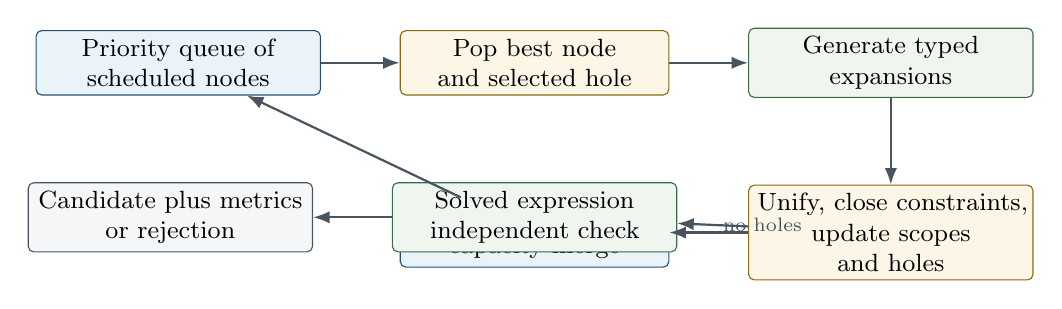
\begin{tikzpicture}[node distance=8mm and 10mm]
  \node[box,text width=34mm] (queue) {Priority queue of\\scheduled nodes};
  \node[goldbox,right=of queue,text width=32mm] (pop) {Pop best node\\and selected hole};
  \node[greenbox,right=of pop,text width=34mm] (expand) {Generate typed\\expansions};
  \node[goldbox,below=11mm of expand,text width=34mm] (unify) {Unify, close constraints,\\update scopes and holes};
  \node[box,left=of unify,text width=32mm] (score) {Score, depth-filter,\\capacity-merge};
  \node[greenbox,below=11mm of pop,text width=34mm] (solved) {Solved expression\\independent check};
  \node[graybox,left=of solved,text width=34mm] (candidate) {Candidate plus metrics\\or rejection};

  \draw[flow] (queue) -- (pop);
  \draw[flow] (pop) -- (expand);
  \draw[flow] (expand) -- (unify);
  \draw[flow] (unify) -- (score);
  \draw[flow] (score) -- (queue);
  \draw[flow] (unify) -- node[right,note]{no holes} (solved);
  \draw[flow] (solved) -- (candidate);
\end{tikzpicture}
\caption{The Exference search loop. Queue pruning and depth pruning are measured, not inferred after the fact. Solved nodes bypass the queue and enter a separate checking path.}
\label{fig:exference-loop}
\end{figure}

\subsection{Queue capacity and exact pruning}

A bounded queue keeps the search operational in large libraries. The merge routine must retain the best nodes under the ordering while reporting exactly how many were discarded. It cannot append two queues, truncate, and then guess which source lost nodes. Those exact counts become \code{QueueLimitPruned} and contribute to progress.

Depth pruning is recorded separately. A final empty queue after any pruning means ``no remaining node under this policy,'' not ``the type is impossible.''

\subsection{Expansion families}

Depending on the goal, expansion can:

\begin{itemize}
  \item introduce a lambda binder;
  \item open or preserve a forall;
  \item choose a local or global binding and create argument holes;
  \item insert visible type applications from exact evidence;
  \item construct a tuple or data constructor;
  \item eliminate a tuple or data value through a case;
  \item use a provider with an occurrence-local assignment;
  \item introduce a let or reuse a previously built value;
  \item carry or discharge class obligations.
\end{itemize}

Every expansion updates the expression and the type state together. A term edge without the corresponding substitution, scope, and hole changes is not a valid child node.

\section{Scoring and usage}

The score combines structural complexity, configured binding ratings, type complexity, depth, class burden, provider penalties, usage policy, and other heuristic features. Source ratings are inputs, not proof evidence. Leant can supply relevance-biased overrides for providers discovered from the current environment.

Usage counts serve several purposes. They can prefer candidates that use requested arguments, reject candidates with unused binders under a strict lane, and provide backend metrics. The strict and relaxed policies are often run as separate lanes rather than one score penalty, because ``unused forbidden'' is a semantic filter while ``unused discouraged'' is a heuristic.

\section{Expression representation}

\dpath{exference/src-core/Language/Haskell/Exference/Core/Expression.hs} wraps the shared generated syntax with annotated locals carrying internal identifiers and optional type information. Compatibility pattern synonyms preserve older Exference-facing constructors while the storage representation converges on the shared AST.

The conversion boundary erases search-only annotations only after scope and typing checks. This is another example of keeping a richer internal proof object until the last responsible moment.

\section{The independent expression checker}\label{sec:exference-checker}

\dpath{exference/src-core/Language/Haskell/Exference/Core/ExpressionCheck.hs} is the key trust boundary. It does not accept the search node's accumulated typing story as a derivation. It reconstructs the expression bidirectionally against an opaque prepared checker context.

The checker validates:

\begin{itemize}
  \item generated-tree well-formedness and absence of holes;
  \item local binder scope and global source identity;
  \item applications, lambdas, tuples, constructors, lets, and cases;
  \item nested forall introduction and visible type application;
  \item rigid-scope provenance and absence of escaping rigids;
  \item constructor/deconstructor schemes;
  \item class givens and residual obligations;
  \item exact equality between reconstructed and claimed residual constraints.
\end{itemize}

It reuses the pure unification kernel because duplicating unification would create two semantics. It does not reuse the search scheduler, queue ordering, score, or node-local assumption that a hole had a certain type. Search contributes only irreducible provenance that cannot be recovered from the erased expression, such as the origin of certain nested rigid instantiations.

The simplified candidate is checked first. If simplification changed a representation in a way the checker rejects, the raw expression may be checked as a fallback. A candidate that fails both is dropped with diagnostics; it is not exposed as ``probably typed.''

\begin{designbox}
The independent checker turns Exference from a heuristic term generator into a checked heuristic term generator. The search can be aggressively optimized or reordered without making every optimization part of the trusted typing argument.
\end{designbox}

\section{Adapter output and defensive rendering}

The stable adapter converts checked internal candidates to shared candidates and attaches metrics such as steps, penalty, final queue size, binding usage, and exact pruning totals. Residual constraints and generated scope are validated again.

Diagnostic hints can originate in user or source text and may be cyclic or infinite in a lazy language. Pure rendering observes a bounded prefix and catches synchronous exceptions while preserving asynchronous exceptions. A bad hint must not take down an otherwise valid search result.

\section{Worked trace: applying a provider}

Consider a goal corresponding to \code{(a -> b) -> F a -> F b} with a provider \code{mapF : forall x y. (x -> y) -> F x -> F y}.

\begin{enumerate}
  \item The root forall prefix creates rigid type variables \code{a} and \code{b}.
  \item Arrow introduction puts \code{f : a -> b} and \code{xs : F a} in scope.
  \item The result hole expects \code{F b}.
  \item Selecting \code{mapF} instantiates its two quantified variables. Exact provider evidence correlates \code{x=a} and \code{y=b} at this occurrence.
  \item The instantiated result unifies with \code{F b}; two argument holes are created for \code{a -> b} and \code{F a}.
  \item Local selection fills them with \code{f} and \code{xs}.
  \item The solved expression contains a global provider occurrence plus visible type applications when required by the source scheme.
  \item The independent checker reconstructs the scheme instantiation and local applications.
\end{enumerate}

This trace exercises the features for which Exference's rich state is justified: occurrence-local assignments, explicit instantiation, global/local scope, and ranking of a library-oriented term.

\section{Why Exference does not refute}

Even a completely empty final queue may be the result of:

\begin{itemize}
  \item a finite step limit;
  \item queue-capacity pruning;
  \item depth pruning;
  \item a finite identifier supply;
  \item disabled expansion families;
  \item ranking that starved a productive region before the limit;
  \item an intentionally incomplete provider or declaration projection;
  \item candidate policies such as forbidding unused binders.
\end{itemize}

The adapter reports these conditions precisely. It never upgrades them to a logical proof. Leant's combined mode preserves this asymmetry: an Exference miss cannot cancel or create a Djinn refutation.

\section{Djinn and Exference compared}

\begin{longtable}{@{}L{0.19\textwidth}L{0.36\textwidth}L{0.36\textwidth}@{}}
\toprule
\textbf{Dimension} & \textbf{Djinn} & \textbf{Exference} \\
\midrule
\endhead
Internal object & Formula, sequent state, proof term & Typed expression with holes, scopes, substitutions, queue state \\
Primary strength & Structural/proof-theoretic synthesis and conditional negative evidence & Ranked library/provider-oriented synthesis and richer elimination/instantiation \\
Ordering & Calculus strategy and plan family & Priority score with queue/depth limits \\
Independent validation & Proof checker & Bidirectional expression checker \\
Rank-N treatment & Opaque-by-default formula plans plus checked instantiation axioms & Opaque polytypes, rigid scopes, visible type applications, occurrence-local assignment \\
Negative result & Possible when translation and search are complete & Never promoted to proof of uninhabitability \\
Candidate ranking & Optional, comparatively light & Core design feature with ratings and usage metrics \\
Typical failure question & ``Was translation/search complete?'' & ``Which policy, score, or bound removed the productive node?'' \\
\bottomrule
\end{longtable}

\begin{sourcebox}
The shortest Exference source trail is: \dpath{exference/src-core/Language/Haskell/Djex/Exference.hs} $\rightarrow$ \dpath{exference/src-core/Language/Haskell/Djex/Exference/Internal/Request.hs} $\rightarrow$ \dpath{exference/src-core/Language/Haskell/Exference/Core/Internal/ExferenceNodeBuilder.hs} $\rightarrow$ \dpath{exference/src-core/Language/Haskell/Exference/Core/Internal/Exference.hs} $\rightarrow$ \dpath{exference/src-core/Language/Haskell/Exference/Core/Unify.hs} $\rightarrow$ \dpath{exference/src-core/Language/Haskell/Exference/Core/ExpressionCheck.hs}.
\end{sourcebox}

\chapter{The unified facade, source frontends, and REPL}\label{ch:djex-facade}

\section{A capability-aware facade}

\dpath{src/Language/Haskell/Djex.hs} is the preferred programmatic entry surface. It defines the backend selection, common session/query operations, and an explicit capability vocabulary. Capabilities include deciding inhabitation, heuristic search, prenex polymorphism, rank-N introduction and elimination, opaque rank-N transport, impredicative support, ranked candidates, and type-class constraints.

The capability matrix is executable documentation. A client can choose Djinn when a complete structural negative result matters, Exference when ranking or elimination matters, or both when it can merge candidates while respecting asymmetric evidence.

\begin{invariantbox}
A facade may normalize calling conventions, but it may not normalize away semantic differences. ``No candidates'' has backend-specific meaning and remains so after dispatch.
\end{invariantbox}

\section{Source conversion}

\dpath{src/Language/Haskell/Djex/HaskellSrc.hs} and the historical frontend conversion modules parse Haskell source declarations into the shared environment vocabulary and render generated terms back to Haskell-like source. The conversion boundary handles qualification, operator names, source locations, fixities where supported, class declarations, and the mismatch between source syntax and neutral AST structure.

The historical Exference frontend under \filepath{exference/src-frontend/Language/Haskell/Exference} includes environment parsing, declaration extraction, source-type conversion, class-environment construction, expression rendering, and CLI support. The historical Djinn frontend under \filepath{djinn/src-frontend} retains its original command vocabulary and help surface.

These frontends are useful compatibility layers, but new semantic changes should enter through shared authorities and checked adapters. Adding a type feature only to a source parser creates a value neither backend has promised to understand.

\section{Packages, workspaces, and dependency order}

\dpath{src/Language/Haskell/Djex/Package.hs} and \dpath{src/Language/Haskell/Djex/REPL/Workspace.hs} manage packages and workspaces. A workspace is not merely a list of files. It must resolve module identities, dependencies, declaration order, loaded environments, and command-line tool interaction. \dpath{src/Language/Haskell/Djex/Internal/DependencyGraph.hs} supplies dependency ordering and cycle handling.

Package discovery can invoke Cabal-facing tooling. Test support includes a fake Cabal executable so CLI behavior can be tested without making unit tests depend on a user's machine configuration. On the current branch there are two such fixtures: \code{djex-fake-cabal} and a \code{djex-fake-z3} solver stand-in used by the live Length suites; Leant's own unit test suite declares a \code{Build-Tool-Depends} on \code{djex:djex-fake-z3} for the same reason.

\section{The unified REPL}

The large \dpath{src/Language/Haskell/Djex/REPL.hs} coordinates the interactive session. Focused submodules divide concerns:

\begin{longtable}{@{}L{0.31\textwidth}L{0.61\textwidth}@{}}
\toprule
\textbf{Module} & \textbf{Responsibility} \\
\midrule
\endhead
\dpath{src/Language/Haskell/Djex/REPL/Command.hs} & Command grammar, abbreviations, arguments, and command-level diagnostics. \\
\dpath{src/Language/Haskell/Djex/REPL/Driver.hs} & Input loop, prompt, multiline behavior, output and exception boundary. \\
\dpath{src/Language/Haskell/Djex/REPL/Scope.hs} & Visible declarations, qualification, ambiguity, namespace resolution, and import/export effects. \\
\dpath{src/Language/Haskell/Djex/REPL/Type.hs} & Type parsing, normalization, checking, and user-facing type operations. \\
\dpath{src/Language/Haskell/Djex/REPL/Kind.hs} & Kind queries and diagnostics. \\
\dpath{src/Language/Haskell/Djex/REPL/Eval.hs} & Evaluation-oriented commands and source execution boundaries. \\
\dpath{src/Language/Haskell/Djex/REPL/DjinnScope.hs} & Projection of the unified visible scope into Djinn-specific premise policy. \\
\dpath{src/Language/Haskell/Djex/REPL/Workspace.hs} & Workspace loading, module graph, package context, and reload behavior. \\
\bottomrule
\end{longtable}

The top-level REPL maintains both source-facing state and backend sessions. A declaration update must rebuild or increment every dependent authority in a defined order. The REPL should never retain an Exference session built from environment version \(n\) while rendering against source scope version \(n+1\).

\section{Commands and the CLI}

\dpath{src/Language/Haskell/Djex/Command.hs} defines shared command structures, while \dpath{src/Language/Haskell/Djex/CLI.hs} handles process arguments, modes, files, and startup behavior. \dpath{src/Language/Haskell/Djex/Text.hs} centralizes bounded text helpers and presentation details.

The three executables are intentionally thin at their \filepath{app/Main.hs} entry points. Substantive process behavior lives in library modules, which is why CLI tests can call command logic without forking for every assertion while still retaining end-to-end executable tests.

\section{Extension discipline}

A safe feature generally lands in this order:

\begin{enumerate}
  \item add or refine a shared authority and its pure tests;
  \item update environment/inventory validation and kind inference;
  \item teach Djinn's adapter/compiler only what it can soundly translate;
  \item teach Exference's adapter/unifier/search/checker only what it can reconstruct;
  \item update the generated AST if a genuinely new term form is required;
  \item update source frontends and renderers;
  \item expose a capability bit or diagnostic when support is asymmetric;
  \item add facade, REPL, CLI, and integration tests.
\end{enumerate}

Starting at the REPL and working downward usually creates a period in which text syntax exists without a validated semantic path.

\chapter{Djex tests, benchmarks, and diagnostic workflow}\label{ch:djex-tests}

\section{Concentric test layers}

The repository's test organization mirrors its trust boundaries.

\begin{longtable}{@{}L{0.28\textwidth}L{0.64\textwidth}@{}}
\toprule
\textbf{Suite} & \textbf{What it protects} \\
\midrule
\endhead
\dpath{synthesis/test/Spec.hs} & Shared names, types, substitution, alpha equivalence, environments, kind inference, queries, generated syntax, inventories, finite-width guards, and diagnostics. \\
\dpath{djinn/test-unit/Spec.hs} & Formula translation, LJT rules, normalization, instantiation plans, proof checking, lowering, evidence, budgets, and regressions. \\
\dpath{djinn/test-property/PropertySpec.hs} & Property-level relationships such as checker acceptance, normalization, and generated-term invariants over broad inputs. \\
\dpath{exference/test-unit/Spec.hs} & Unification, rigid scopes, class closure, node expansion, scoring, provider assignments, expression checking, pruning, and regressions. \\
\dpath{exference/test-engine/EngineSpec.hs} & Black-box engine behavior with checked environments and bounded search. \\
\dpath{test-api/AbstractionBoundary.hs} & Compile-time enforcement that internal constructors and modules do not leak through the supported public API. \\
\dpath{test-api/FacadeSpec.hs} & Backend dispatch, capability reporting, common query behavior, and facade diagnostics. \\
\dpath{test-integration/Spec.hs} & Cross-layer behavior: source declarations through sessions and engines to rendered candidates and evidence. \\
\dpath{test-cli/Spec.hs} & Unified command-line and REPL protocol, formatting, files, workspaces, package discovery, and failure behavior. \\
Historical CLI/API suites & Compatibility of the retained \code{djinn} and \code{exference} entry surfaces. \\
\filepath{synthesis/test-length} (current branch) & The Length/SpinePair behavioral domains: SMT-LIB planning, protocol, session, causal transport, and live execution against the \code{djex-fake-z3} fixture. \\
\filepath{synthesis/test-certificate} (current branch) & The package-private certificate-plan foundation and typed-candidate association, compiled as home modules so sealed invariants are testable without public construction. \\
\filepath{synthesis/test-fingerprint} (current branch) & The private fingerprint builder and behavioral-problem sealer. \\
\filepath{synthesis/test-term-graph-fingerprint} (current branch) & Allocation-insensitive structural fingerprints for sealed term graphs. \\
\bottomrule
\end{longtable}

The current-branch \filepath{djex.cabal} declares sixteen test suites in total: the twelve pinned-snapshot suites above plus \code{synthesis-length-tests}, \code{synthesis-certificate-tests}, \code{synthesis-fingerprint-tests}, and \code{synthesis-term-graph-fingerprint-tests}.

The abstraction-boundary tests deserve special attention. In Haskell, a module export list is part of the correctness story. If a constructor becomes public accidentally, downstream code can fabricate a value that bypasses every runtime test. Compile-time negative tests guard that boundary.

\section{Benchmarks}

Both historical engines have benchmark corpora. A useful benchmark change should record more than wall-clock time. For Djinn, track proof-plan counts, choice points, proof prefix latency, and deduplication. For Exference, track steps, peak/final queue size, exact queue/depth pruning, candidate rank, and checker rejection. A speedup that changes the first accepted candidate or turns finished search into truncation is a semantic change and should be reviewed as such.

\section{A practical failure funnel}\label{sec:djex-failure-funnel}

When a top-level test says ``expected candidate, got none,'' localize the loss:

\begin{enumerate}
  \item \term{Source conversion}: did the declaration or goal parse to the intended shared type?
  \item \term{Environment}: did validation retain the declaration and indexes?
  \item \term{Projection}: did the selected backend session include the value, constructor, class, or instance?
  \item \term{Request}: did exact contexts and provider assignments survive checked preparation?
  \item \term{Search}: did the backend generate a proof/node, or did a bound/prune intervene?
  \item \term{Internal checker}: did proof or expression reconstruction reject it?
  \item \term{Shared AST}: did scope, simplification, or candidate conversion reject it?
  \item \term{Frontend}: did qualification or source rendering reject or duplicate it?
\end{enumerate}

Instrumenting all eight at once produces noise. Add a probe at the earliest boundary whose output is wrong.

\section{Negative-evidence tests}

The most valuable negative tests are not examples of impossible types; they are examples where a tempting implementation would falsely claim impossibility. Include cases with:

\begin{itemize}
  \item a search budget reached just before a proof;
  \item an omitted rank-N structural plan;
  \item an opaque nominal type that must be forwarded;
  \item a recursive type whose one-layer exposure is incomplete;
  \item a provider assignment that a plan fails to retain exactly;
  \item target self-reference excluded from the safe environment;
  \item Exference queue/depth pruning followed by an empty queue.
\end{itemize}

These tests protect the distinction between ``no proof exists'' and ``this implementation did not find one.''

\begin{summarybox}
Djex's test suite is best read as a map of trusted boundaries. Pure shared tests establish authorities; backend tests establish search and checking; API tests establish encapsulation; integration and CLI tests establish that the boundaries compose.
\end{summarybox}

\part{Leant}

\chapter{Repository and runtime architecture}\label{ch:leant-model}

\section{Build graph and reproducible pairing}

Leant is a Haskell executable package described by \lpath{leant.cabal}. It depends on Djex as a library, Haskeline for the interactive terminal, process and directory APIs for the Lean backend, and a deliberately small set of utility packages. \lpath{cabal.project} builds the Leant package together with \filepath{lib/Djex}. The latter is a Git submodule declared in \lpath{.gitmodules} and pinned, at this snapshot, to the exact Djex commit used throughout Part II.

That pin is architecturally significant. The bridge imports internal details of the shared generated and query vocabulary that evolve in tandem with provider evidence and rank-N support. A floating package dependency would make it difficult to know whether a candidate-rendering failure came from Leant or an incompatible Djex revision.

The executable is launched directly or through \lpath{leant.cmd} on Windows. The Lean side is not linked into the Haskell process. Leant discovers a Lake project and a Lean REPL executable, then starts that backend as a child process.

\section{The source is intentionally concentrated}

The principal modules are:

\begin{longtable}{@{}L{0.31\textwidth}L{0.61\textwidth}@{}}
\toprule
\textbf{Module} & \textbf{Responsibility} \\
\midrule
\endhead
\lpath{src/Main.hs} & Entry point, command dispatcher, interactive state, ordinary Lean command execution, imports, files, undo, reset/reload, generated \code{it} bindings, prove mode, synthesis command orchestration, verification, and user-facing output. \\
\lpath{src/Leant/Backend.hs} & Backend discovery, child-process lifecycle, UTF-8 handles, request framing, timeouts, server death, bounded stderr capture, and low-level errors. \\
\lpath{src/Leant/Json.hs} & Dependency-light JSON AST, parser, and encoder used by the backend protocol. \\
\lpath{src/Leant/Classify.hs} & Lexical command classification and multiline continuation heuristic; it is deliberately not the Lean parser. \\
\lpath{src/Leant/Format.hs} & Source-like formatting of selected \code{#print} output. \\
\lpath{src/Leant/Builtins.hs} & Static help for Lean syntax and keywords that are not ordinary environment constants. \\
\lpath{src/Leant/Session/Replay.hs} & Pure transactional replay accumulator for environments, history, undo stack, and generated \code{it} counters. \\
\lpath{src/Leant/Session/Snapshot.hs} & Snapshot metadata, fingerprinting, companion artifacts, validation, durable temporary ownership, and atomic publication. \\
\lpath{src/Leant/Synth/Fragment.hs} & Lean payload serializer source, S-expression parser, \code{Frag} grammar, provider metadata, fragment analyses, recursive-family completeness, and classical/structural transformations. \\
\lpath{src/Leant/Synth/Engine.hs} & Fragment-to-Djex translation, Djinn and Exference sessions, provider assignments, library premises, staged engine runs, candidate merging, evidence policy, and bounded forcing. \\
\lpath{src/Leant/Synth/Render.hs} & Neutral generated-AST fitting to exact Lean binders, premise removal, provider replacement, pattern normalization, naming, textual variants, and Lean source rendering. \\
\lpath{src/Leant/Synth/ProviderCache.hs} & Semantic provider query keys, provider-world generations, and bounded recency cache. \\
\lpath{src/Leant/Synth/Replay.hs} & Pure decision whether a derived synthesis environment can be reused, replayed by suffix, or rebuilt. \\
\filepath{src/Leant/Synth/Observability.hs} (current branch) & Typed-route eligibility vocabulary: \code{CandidateRenderingRoute}, \code{VerificationFailureClass}, and \code{LeantSynthesisMetric}. \\
\bottomrule
\end{longtable}

The architecture is asymmetrical: the pure and trust-sensitive transformations are factored into focused modules, while orchestration remains concentrated in \code{Main.hs}. This makes a top-down read feasible---almost every command begins in one file---but it also means changes to state ownership must be made carefully. A future refactor can extract command families and synthesis orchestration without moving the pure fragment/engine/render boundaries.

\section{Runtime components}

\begin{figure}[htbp]
\centering
\resizebox{0.98\textwidth}{!}{%
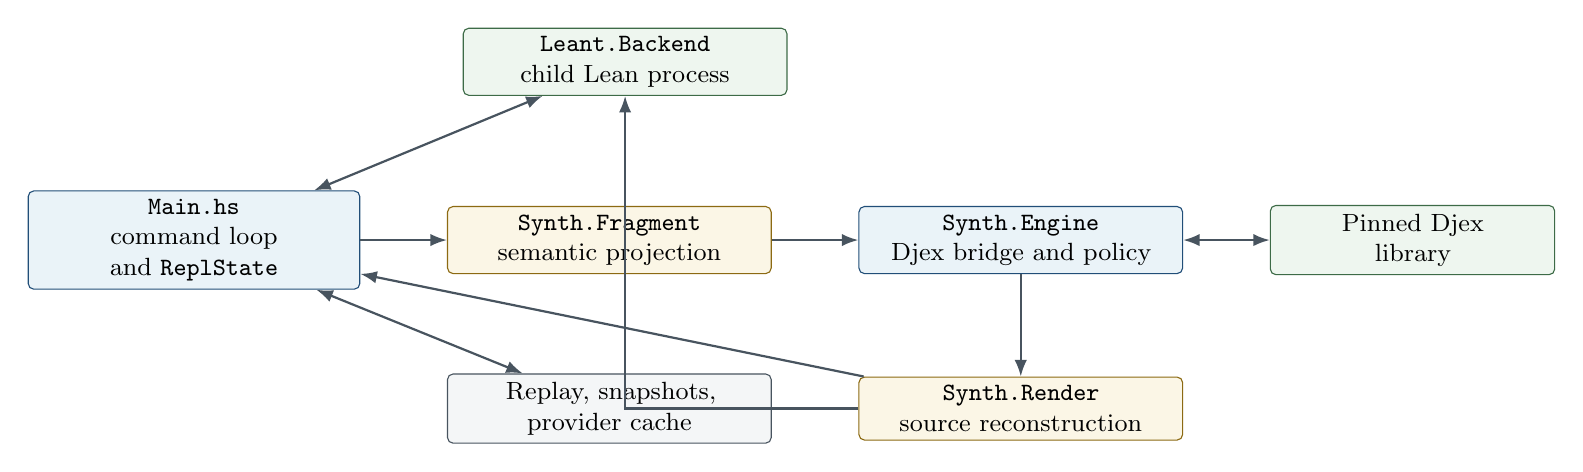
\begin{tikzpicture}[node distance=8mm and 11mm]
  \node[box,text width=40mm] (main) {\code{Main.hs}\\command loop and \code{ReplState}};
  \node[greenbox,above right=12mm and 13mm of main,text width=39mm] (backend) {\code{Leant.Backend}\\child Lean process};
  \node[goldbox,right=of main,text width=39mm] (fragment) {\code{Synth.Fragment}\\semantic projection};
  \node[box,right=of fragment,text width=39mm] (engine) {\code{Synth.Engine}\\Djex bridge and policy};
  \node[greenbox,right=of engine,text width=34mm] (djex) {Pinned Djex\\library};
  \node[goldbox,below=13mm of engine,text width=39mm] (render) {\code{Synth.Render}\\source reconstruction};
  \node[graybox,left=of render,text width=39mm] (session) {Replay, snapshots,\\provider cache};

  \draw[backflow] (main) -- (backend);
  \draw[flow] (main) -- (fragment);
  \draw[flow] (fragment) -- (engine);
  \draw[backflow] (engine) -- (djex);
  \draw[flow] (engine) -- (render);
  \draw[flow] (render) -- (main);
  \draw[backflow] (main) -- (session);
  \draw[flow] (render) -| (backend);
\end{tikzpicture}}
\caption{Leant's principal module/runtime relationships. The child Lean process is used at both ends: to project the goal and to verify reconstructed candidates.}
\label{fig:leant-modules}
\end{figure}

\section{Startup}

A representative startup path in \code{Main.hs} is:

\begin{enumerate}
  \item normalize console and buffering behavior; on Windows, request UTF-8 code pages and virtual-terminal support;
  \item inspect command-line arguments and environment overrides;
  \item discover the current Lake project by walking ancestor directories;
  \item discover the Lean REPL executable, including the LeanInteract cache convention;
  \item create a \code{BackendConfig};
  \item start the backend lazily or eagerly according to the command path;
  \item establish the initial Lean environment and baseline imports;
  \item initialize Haskeline and the large \code{ReplState};
  \item enter the command loop.
\end{enumerate}

The backend may die later. Startup is therefore not a one-time phase; the same discovery/configuration data supports replacement processes and transactional reconstruction.

\chapter{The Lean backend protocol and small support modules}\label{ch:leant-backend}

\section{Backend configuration and discovery}

\lpath{src/Leant/Backend.hs} defines a configuration containing the Lake executable or path, the Lean REPL executable, and the working directory/project. Discovery respects explicit environment configuration before probing caches and ancestors. The command is assembled as a Lake environment invocation so the backend sees the exact package search path and toolchain selected by the project.

The working directory matters. Running the same binary outside the Lake root can change import resolution, output artifacts, and environment fingerprints. Leant carries the directory in configuration rather than relying on a mutable process-global current directory.

\section{Process creation}

The child process is created with piped standard input, output, and error. The handles are configured for UTF-8 and line buffering. Backend state owns the process handle and all three pipes. Ownership is singular: when a request times out or the server closes, Leant terminates and discards the whole backend value rather than leaving a half-valid handle set in the main state.

The stderr pipe is not merged with stdout because stdout is a framed data protocol. Stderr is captured continuously on a dedicated thread and bounded by bytes, not lines: only the newest \code{maximumCapturedStderrBytes} = 64~KiB tail is retained, and a truncation flag records whether earlier output was dropped. On server death, the drain waits only briefly for capture completion, so diagnostics cannot hang reconstruction forever.

\section{Request framing}

Leant sends one JSON object followed by a blank line and flushes. It reads response lines until a blank line, joins them, and parses the result as JSON. The blank-line delimiter lets the Lean backend emit formatted JSON over several lines without requiring a binary length prefix.

The framing layer distinguishes three principal failures:

\begin{itemize}
  \item \code{ServerClosed}: the child exited or closed stdout; bounded stderr is attached when available;
  \item \code{RequestTimeout}: the configured wall-clock request limit elapsed;
  \item \code{BadResponse}: a complete frame arrived but was not valid JSON or did not have the expected structure.
\end{itemize}

A timeout is treated more severely than an ordinary Lean error in the JSON payload. The process may still be computing or may have emitted a partial frame, so Leant kills it and marks the session for replay on the next command.

\begin{invariantbox}
A backend process and a Lean environment identifier form one lease. After timeout or transport death, no old environment identifier may be sent to a replacement process. Reconstruction must establish new identifiers in the new process first.
\end{invariantbox}

\section{The local JSON implementation}

\lpath{src/Leant/Json.hs} defines a compact JSON value type and hand-written parser/encoder. It supports objects, arrays, strings, numbers, Booleans, and null; string parsing handles escapes, Unicode escapes, and surrogate pairs.

Keeping JSON local has two advantages. First, the protocol surface stays explicit and small; error messages can mention the exact expected shape. Second, snapshot and interactive behavior are not coupled to a large generic encoding layer whose defaults might change field order, number handling, or duplicate-key policy.

The module should be treated as protocol infrastructure. Changes need round-trip tests, malformed-input tests, escaped-control tests, and non-BMP character tests. A permissive parser can be dangerous here: accepting trailing garbage may desynchronize frame handling.

\section{Lexical classification, not parsing}

\lpath{src/Leant/Classify.hs} answers practical questions before sending text to Lean: Does the line begin a top-level declaration? Are delimiters balanced? Does the user likely intend another line? It strips or ignores string literals, character literals, line comments, and nested block comments while scanning.

It does not decide whether Lean syntax is valid. The backend remains the parser authority. The classifier is allowed to be conservative: asking for one extra continuation line is inconvenient; prematurely sending half a declaration is destructive to interactive flow.

The top-level keyword set includes declaration forms and command prefixes used to classify history and provider-world invalidation. Any new Lean syntax added here should be tested inside comments and strings so false positives do not alter state.

\section{Formatting and built-in help}

\lpath{src/Leant/Format.hs} reshapes selected \code{#print} output into readable Lean-style declarations. It recognizes inductive, structure, and class layouts and indents definitions. This is presentation logic over backend output, not a parser used for synthesis.

\lpath{src/Leant/Builtins.hs} fills a different gap. Lean keywords and syntax forms such as tactical constructs do not necessarily appear as environment constants. Static help entries make them discoverable without pretending they have ordinary types.

\begin{designbox}
Leant has three deliberately separate text readers: the JSON protocol parser, the lightweight command classifier, and Lean itself. Reusing the classifier to interpret declarations or reusing formatted \code{#print} text as semantic type evidence would cross trust boundaries in the wrong direction.
\end{designbox}

\chapter{Interactive state and command execution}\label{ch:leant-state}

\section{Reading \code{ReplState} by ownership domain}

The record in \code{Main.hs} is large, but its fields form coherent groups.

\begin{longtable}{@{}L{0.24\textwidth}L{0.68\textwidth}@{}}
\toprule
\textbf{Domain} & \textbf{Representative state and invariant} \\
\midrule
\endhead
Backend lease & Optional process, immutable backend configuration, project directory, timeout. Environment IDs are meaningful only inside the current process. \\
Interactive Lean state & Current environment ID, base environment, snapshot base, imports, replayable history, undo stack, loaded-file identity and timestamps. \\
Derived environment state & Browse environment, synthesis base/environment, cached replay prefix. These may lag only when explicitly marked invalid and must be rebuilt before use. \\
Generated-value state & \code{it} counter, most recent \code{sorry}, private generated names, completion cache. Generated bindings have special invalidation rules. \\
Synthesis state & Engine choice, steps/budgets, classical/library switches, ratings, provider world and cache, synthesis-scoped generated splices. \\
Prove-mode state & Current proof session, goal information, splice counter, proof-local candidates. Leaving prove mode must remove or invalidate them. \\
Presentation state & Color mode, interactivity, timing, transcript capture, output sink, prompt/completion behavior. \\
\bottomrule
\end{longtable}

The state record is mutable through Haskell updates, but many operations construct a complete replacement substate before installing it. The code is easiest to reason about when every field is assigned one of three roles: durable replay input, process-local handle, or derived cache.

\section{Ordinary command execution}

For a non-colon Lean command, the loop roughly performs:

\begin{enumerate}
  \item classify and collect a complete input block;
  \item ensure a live backend, replaying the session when required;
  \item build a request payload containing the current environment ID and command;
  \item run it under the configured timeout;
  \item inspect backend errors, messages, and the new environment ID;
  \item if successful, call the state-advance path to append history and push the previous state onto the undo stack;
  \item invalidate derived browse/synthesis/provider data according to the declaration's semantic effect;
  \item format and emit messages through the centralized output path.
\end{enumerate}

The central \code{emit} function is more than convenience. Transcript capture, tests, color policy, and interactive output all observe the same sequence. Code that writes directly to stdout can make snapshots or golden tests appear nondeterministic.

\section{Advancing environments}

The state advance function updates the current Lean environment, replay history, undo stack, generated-value counter, and derived cache validity as one operation. Ordinary user declarations increment the provider-world generation and clear provider/completion caches. Generated \code{it} declarations are treated specially: they make the value available to subsequent commands but do not invalidate the provider world, because otherwise every synthesis result would evict the provider discovery that produced it.

This distinction is semantic, not based solely on a textual prefix. Generated definitions use a private mangled name convention and are recognized during replay and scanning.

\section{Generated \code{it} bindings}\label{sec:leant-it}

Leant gives verified values convenient names \code{it}, \code{it1}, and so on, but it cannot safely declare those ordinary names repeatedly. Internally it uses private generated names carrying a monotonically increasing counter. A source scanner rewrites bare references to the friendly names outside strings and comments. Output is rewritten in the opposite direction.

The scanner must understand enough lexical structure to avoid changing:

\begin{itemize}
  \item a substring inside a longer identifier;
  \item string and character literals;
  \item line comments and nested block comments;
  \item already mangled generated names;
  \item numeric suffixes that refer to older results.
\end{itemize}

Verified synthesis results are installed from worst to best. The newest generated definition is therefore the highest-ranked survivor and receives the bare \code{it} view. This order also makes undo intuitive: undoing once removes the best result first and reveals the next generated value if present.

A generated definition may require \code{noncomputable}. Leant first tries the ordinary declaration and retries with the modifier when the backend reports the relevant failure. Only successful declarations enter history.

\section{Undo}

The undo stack stores enough state to restore the prior environment and history boundary. Undo cannot cross the durable snapshot base because the older process-local environment IDs no longer exist and the snapshot deliberately defines a reconstruction root.

On undo, Leant restores:

\begin{itemize}
  \item the previous environment ID;
  \item replay history length and contents;
  \item synthesis-derived state or invalidation markers;
  \item the generated \code{it} counter derived from surviving history;
  \item provider-world/cache state according to whether an ordinary declaration was removed.
\end{itemize}

The counter is not merely decremented blindly. Replay and undo scan recognized generated names so gaps or a loaded snapshot cannot cause name reuse.

\section{Reset, reload, and load}

These commands intentionally differ in reconstruction policy.

\begin{itemize}
  \item \code{:reset} starts a replacement backend without replaying the old history. It preserves user preferences such as timeout, color, engine, and search settings while clearing definitions and any loaded snapshot to the baseline; imports are kept---the help text reads ``clear definitions/snapshot (keeps imports)''---and newly listed imports take effect on the next \code{:reset}.
  \item \code{:reload} re-executes the currently loaded file against a fresh appropriate base, replacing its prior effects.
  \item \code{:load} starts without replaying the old session and establishes a new file/import/history root.
\end{itemize}

The ``without replay'' path is crucial. If history itself contains a command that now crashes the backend, a recovery command must not execute that command before it gets a chance to clear or replace the state.

\begin{pitfallbox}
A generic \code{ensureBackend} that always replays history before dispatch would make \code{:reset}, \code{:load}, and snapshot restoration unusable precisely when they are needed most. Replacement-process creation and old-session replay are separate operations in Leant.
\end{pitfallbox}

\chapter{Transactional replay and snapshots}\label{ch:leant-recovery}

\section{Why replay is transactional}

After a timeout or server death, all old Lean environment IDs are invalid. Leant must create a replacement process and reproduce the session from durable inputs. A naive implementation might update \code{ReplState} after every replayed command. If command \(k\) fails, the interactive state would then point partly into the new process while history, undo, caches, and snapshot ownership still describe the old process.

Leant instead constructs a \code{ReconstructedSession} off to the side. Only after snapshot/import restoration and every history command succeed does it install the new backend and environment IDs. On failure, the partial replacement process is terminated and the old logical state remains available for reset or diagnostic commands.

\section{Reconstruction sources}

A session has one of two principal roots:

\begin{enumerate}
  \item a base Lean environment plus a replayable import sequence;
  \item a validated snapshot artifact with companion metadata and optional tooling artifact.
\end{enumerate}

From that root, Leant replays ordinary history commands in order. The derived browse and synthesis environments are invalidated or replayed independently because their payloads and purposes differ from the interactive environment.

\section{Pure replay accumulation}

\lpath{src/Leant/Session/Replay.hs} contains the pure accumulator. Given a starting environment and a sequence of successfully executed history records, it computes the resulting current environment, undo boundaries, surviving history, and generated \code{it} counter. If any command fails at the effectful layer, no partial accumulator is returned as installable state.

Generated names are recognized during replay. This preserves counters across process replacement and prevents a newly synthesized \code{it} from colliding with a replayed definition.

Undo entries cannot precede the reconstruction root. If a snapshot compacted a long history, the new undo stack begins at the snapshot base even though the source session had older commands.

\section{Import reconstruction}

A Lean backend may report success while ignoring or degrading a missing import in ways that are not obvious from one response field. The import reconstruction path therefore probes the resulting environment after imports and records the actual base. This avoids installing a session whose history IDs are valid but whose declaration universe differs from the old one.

\section{Snapshot structure}

These mechanics surface interactively as the \code{:pickle FILE} and \code{:unpickle FILE} commands: \code{:pickle} saves the current environment plus its synthesis companion, and \code{:unpickle} restores a validated family as a new undo/history base. \lpath{src/Leant/Session/Snapshot.hs} manages such a snapshot as a small artifact family:

\begin{itemize}
  \item the upstream Lean environment artifact, normally an \filepath{.olean};
  \item an optional tooling companion needed by the interactive backend;
  \item a versioned sidecar containing format metadata, sibling names, fingerprints, sizes, and synthesis-tooling ABI information;
  \item durable temporary copies owned by a \code{SnapshotBase} value while the session is live.
\end{itemize}

The sidecar's fingerprint is a streaming FNV-1a 64-bit value accompanied by byte count. It is explicitly a corruption/identity check, not a cryptographic signature. The tooling ABI fingerprint incorporates serializer and prelude source so a snapshot created by an incompatible synthesis bridge is rejected rather than used with subtly different fragment semantics.

\subsection{Validation}

Snapshot loading checks:

\begin{itemize}
  \item sidecar format version;
  \item expected sibling filenames and presence;
  \item byte sizes and fingerprints;
  \item tooling ABI compatibility;
  \item whether optional companions are consistently declared and present.
\end{itemize}

Only a validated artifact family becomes a \code{SnapshotBase}. The temporary ownership type ensures files needed by the live session are not deleted while state still refers to them.

\subsection{Publication}

Publishing a snapshot uses temporary names, sibling placement, rename, backup, and restore. This protects an existing valid snapshot if publication of a new family fails halfway through. The implementation accounts for Windows rename semantics, where replacing an existing file is less uniform than on POSIX systems.

\begin{figure}[htbp]
\centering
\resizebox{0.96\textwidth}{!}{%
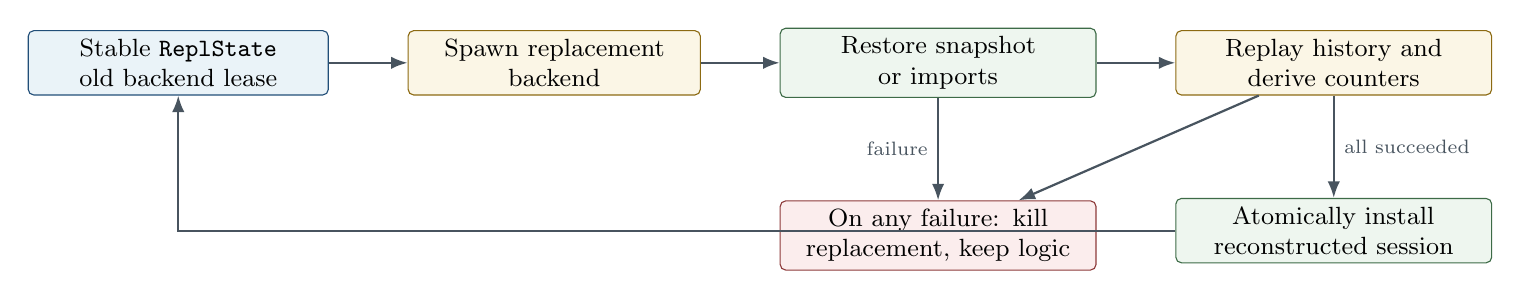
\begin{tikzpicture}[node distance=8mm and 10mm]
  \node[box,text width=36mm] (old) {Stable \code{ReplState}\\old backend lease};
  \node[goldbox,right=of old,text width=35mm] (spawn) {Spawn replacement\\backend};
  \node[greenbox,right=of spawn,text width=38mm] (root) {Restore snapshot\\or imports};
  \node[goldbox,right=of root,text width=38mm] (replay) {Replay history and\\derive counters};
  \node[greenbox,below=13mm of replay,text width=38mm] (install) {Atomically install\\reconstructed session};
  \node[redbox,below=13mm of root,text width=38mm] (discard) {On any failure: kill\\replacement, keep logic};

  \draw[flow] (old) -- (spawn);
  \draw[flow] (spawn) -- (root);
  \draw[flow] (root) -- (replay);
  \draw[flow] (replay) -- node[right,note]{all succeeded} (install);
  \draw[flow] (root) -- node[left,note]{failure} (discard);
  \draw[flow] (replay) -- (discard);
  \draw[flow] (install.west) -| (old.south);
\end{tikzpicture}}
\caption{Transactional process reconstruction. The old logical state is never mutated into a half-replayed state.}
\label{fig:leant-replay}
\end{figure}

\section{Derived synthesis replay}

\lpath{src/Leant/Synth/Replay.hs} contains a pure prefix comparison returning one of three decisions:

\begin{itemize}
  \item \code{Reuse}: cached derived synthesis state already corresponds exactly to current history;
  \item \code{ReplaySuffix}: cached history is a prefix, so only the new suffix must be executed in the synthesis environment;
  \item \code{ReplayAll}: histories diverge or the cache is invalid, so rebuild from the synthesis base.
\end{itemize}

This small module prevents the large main loop from embedding subtle prefix logic in several command paths. It also makes replay decisions independently testable.

\section{Recovery scenarios}

\subsection{Timeout during an ordinary command}

The request path kills the backend and marks it absent. No new environment ID or history item is installed. The next command that needs Lean starts a replacement and replays the prior committed session. The timed-out command is not automatically retried, because its completion status is unknown.

\subsection{Server death during synthesis verification}

The candidate is not accepted. The backend lease is dropped. Djex state can remain in memory, but every Lean environment identifier and provider serialization tied to the dead process is treated as invalid until reconstruction. The next user command triggers replay.

\subsection{Unreplayable history}

Normal commands report replay failure without installing the partial replacement. The user can still issue \code{:reset}, \code{:load}, or snapshot restoration because those commands create a replacement without replaying the bad history first.

\begin{summarybox}
Leant treats process death as loss of process-local identity, not loss of the logical session description. History, imports, snapshots, and settings are durable inputs; environment identifiers, handles, and derived caches are leases that can be reconstructed.
\end{summarybox}

\chapter{From Lean expressions to the synthesis fragment}\label{ch:leant-fragment}

\section{Why the bridge needs its own language}

Lean's elaborated expression language is far more expressive than Djinn's logic or Exference's type language. It contains dependent products, universe levels, metavariables, reducibility, projections, recursors, quotient machinery, coercions, type-class synthesis artifacts, and arbitrary constants. A direct recursive translation would either reject nearly every practical goal or silently erase dependencies.

Leant instead defines a fragment that serves three purposes at once:

\begin{enumerate}
  \item a \term{search projection}: the structural type problem sent to Djex;
  \item a \term{rendering guide}: exact binder, constructor, application, and provider metadata needed to reconstruct Lean source;
  \item a \term{completeness ledger}: explicit reasons why a no-candidate result may or may not support a negative conclusion.
\end{enumerate}

The implementation is in \lpath{src/Leant/Synth/Fragment.hs}. The module contains both the source of the Lean serializer payload and the Haskell parser/analysis code, keeping producer and consumer close enough to review together.

\section{The serializer runs after elaboration}

The payload uses Lean metaprogramming to inspect the elaborated target and relevant declarations. It is embedded as source text and sent through the backend. Running after elaboration gives it exact binder info, fully resolved constant names, instantiated universes, inductive metadata, and local context. It does not need to reverse-engineer surface notation such as \code{A x B} versus \code{Prod A B}.

The payload emits a small S-expression protocol rather than JSON. The format is optimized for recursive tagged trees and can be parsed with bounded, location-aware routines in Haskell. Strings and exact names are quoted or escaped by the producer; the consumer does not split on whitespace heuristically.

The serializer carries a depth budget. When the budget is reached, it emits an explicit \code{FDepth}-like marker. It does not replace deep structure with a plausible atom. This distinction is what later prevents a depth-limited projection from supporting refutation.

\section{The \code{Frag} grammar}

The principal constructors can be grouped as follows.

\begin{longtable}{@{}L{0.26\textwidth}L{0.64\textwidth}@{}}
\toprule
\textbf{Fragment form} & \textbf{Meaning} \\
\midrule
\endhead
\code{FArr a b} & Non-dependent function space selected for structural synthesis. \\
\code{FProd xs}, \code{FSum xs} & Product and sum structure, including binary and generalized views used by constructor translation. \\
\code{FTop}, \code{FBot} & Canonical inhabited and empty proposition-like forms. \\
\code{FAll visibility name body} & Sort-level universal binder; visibility records whether Lean expects an explicit or implicit source binder/application behavior. \\
\code{FInst display body} & Instance-implicit binder retained as a distinct slot. Legacy or unsupported forms can be represented but poison negative evidence. \\
\code{FExactContext class args body} & Exact class/context binder with structured argument metadata instead of a flattened atom. \\
\code{FVar key} & Bound structural variable whose identity is tracked through the serializer. \\
\code{FAtom safe key} & Opaque atomic source type. The safety bit says whether treating it as an uninterpreted atom is conservative for refutation. \\
\code{FApp safe key head args} & Retained nominal or higher-kinded application with exact head metadata and projected arguments. \\
\code{FParamInd}, \code{FInd} & Nonrecursive inductive families, with constructor and parameter metadata needed for structural translation and rendering. \\
\code{FParamRec}, \code{FRec} & Recursive families plus an explicit completeness classification and constructor schemas. \\
\code{FDepth} & The serializer stopped because of the projection bound; positive transport may still be possible, negative evidence is incomplete. \\
\bottomrule
\end{longtable}

The exact constructor fields are richer than the summary above. In particular, inductive nodes carry canonical keys, displayed names, parameter counts, constructors, recursive occurrence information, and flags controlling which structural view is safe.

\subsection{Safe and unsafe atoms}

An atom built only from universally bound variables can often be treated as an uninterpreted proposition without making an impossible goal easier. A constant application whose hidden definition might expose constructors or implications cannot safely support the same negative argument. The serializer therefore labels atoms with a safety bit derived from source structure.

Positive synthesis is less demanding. A generated term can forward an unsafe atom as an opaque value and Lean will verify it. The bit becomes decisive only when Leant considers promoting a Djinn miss to refutation.

\subsection{Exact contexts}

Lean instance arguments are dependent function binders with special elaboration behavior. Flattening them to ordinary arrows would make generated terms mention dictionaries as explicit term arguments and would lose class-head correlations. \code{FExactContext} retains the class name and structured arguments. Provider discovery and rendering can then distinguish a constraint required to use a declaration from a normal premise available to arbitrary search.

\subsection{Application heads}

\code{FApp} retains a nominal head rather than pretending every application is structurally transparent. The head metadata separates proper-kinded direct applications from higher-kinded or partially applied heads. This feeds two later paths:

\begin{itemize}
  \item the Djex translation can preserve exact higher-kinded provider assignments;
  \item the renderer can decide whether an argument is a genuine first-order fragment substitution or must remain source metadata.
\end{itemize}

\section{Binder spines and slots}

The renderer needs to align a generated lambda spine with Lean's original products. \code{Fragment.hs} therefore exposes a \code{Slot} view for leading arrows, explicit/implicit universal binders, and instance binders. A slot is not merely a type: it records source visibility and whether a generated term should contain a binder, a placeholder, or no textual argument.

For example, these goals can share a similar structural core but require different source text:

\begin{lstlisting}[language=Leanish]
(a : Sort u) -> a -> a
{a : Sort u} -> a -> a
[a : SomeClass] -> ...
\end{lstlisting}

The first has an explicit type-level binder in surface syntax, the second an implicit one, and the third an instance slot. The engine may erase some of this distinction, but the fragment cannot.

\section{Parsed goals and provider fragments}

A \code{ParsedGoal} contains the target fragment, sort/universe classification, provider query, recursive and unsafe metadata, and any pre-serialized library premises. A \code{ProviderFrag} contains the exact Lean name, a fragment for the provider scheme, source binder names, and one or more correlated assignment vectors.

Provider arguments have three important forms:

\begin{itemize}
  \item a proper fragment with a known kind arity;
  \item an exact fragment carrying tags for forall domains that must remain correlated;
  \item a nominal head with already supplied proper arguments and a remaining higher-kinded arity.
\end{itemize}

Kind arity and exact-domain vectors are bounded at the parser boundary. A malformed backend response cannot allocate an unbounded assignment tree in Haskell.

\section{Analysis functions form the completeness ledger}\label{sec:fragment-ledger}

The module contains many small recursive analyses. They should be read as proof obligations, not miscellany:

\begin{itemize}
  \item \code{fragHasDepth} detects bounded serializer truncation;
  \item \code{fragUnsafeAtoms} collects opaque regions unsafe for negative evidence;
  \item \code{fragHasInstanceBinder} and \code{fragHasUnsupportedInstanceBinder} distinguish supported exact contexts from legacy/opaque ones;
  \item \code{fragProviderMayOpen} asks whether provider-oriented forall elimination could expose useful structure;
  \item \code{fragRecKeys} identifies recursive families relevant to constructor premise selection;
  \item \code{fragSpine} and \code{leadingTypeArgs} drive fitting and provider occurrence alignment;
  \item \code{fragVisibleForallVisibilities} preserves explicit/implicit source behavior;
  \item \code{fragRefusal} explains why a fragment cannot be translated for a selected engine;
  \item \code{glivenkoSplit} and \code{propAtoms} characterize the optional classical fallback fragment;
  \item \code{stripRecCtors} creates a library-search variant less likely to be flooded by closed recursive constructor terms.
\end{itemize}

No single Boolean means ``complete.'' The final decision combines serializer depth, atom safety, context support, recursive-family completeness, nominal-application completeness, exact assignment retention, and engine progress.

On the current branch the fragment module also owns the shared binder-hygiene analyses \code{fragVariableNames}, \code{freeFragVariables}, \code{renameFragBinder}, and \code{freshFragBinderFrom}. Both \code{Leant.Synth.Engine} and \code{Leant.Synth.Render} now consume these from \code{Leant.Synth.Fragment} instead of the near-identical private copies each formerly kept.

\begin{invariantbox}
Every lossy projection must leave a machine-readable scar. If a new \code{Frag} constructor can hide a proof-relevant elimination or constructor, its analysis must prevent a candidate-free Djinn result from being reported as a source-level refutation.
\end{invariantbox}

\section{Recursive-family representation}

Recursive inductives are difficult because unfolding them freely yields infinite types, while treating them only as opaque loses useful constructor synthesis and case analysis. Leant serializes a bounded family schema:

\begin{itemize}
  \item a canonical family key and source name;
  \item parameters versus indices;
  \item constructor domains and result indices;
  \item which fields are recursive occurrences;
  \item whether all relevant constructors and argument fragments were serialized completely;
  \item a fallback nominal identity for forwarding.
\end{itemize}

The engine bridge may add conservative constructor premises outside the goal's leading arrow spine. For a recursive goal, these premises enable one-layer construction or elimination without pretending the entire fixed point has been unfolded. Foreign recursive families are excluded from a library premise when their schema is not tied to the current goal or provider query.

\section{Classical transformation}

The fragment module can identify a restricted proposition-shaped region suitable for a Glivenko-style classical fallback. It splits the goal and enumerates proposition atoms without interpreting arbitrary Lean constants. The transformed search is always budgeted and used only for positive candidates. Even if Djinn exhausts the transformed formula, Leant does not report a source-level classical refutation from that lane.

\begin{sourcebox}
Read \lpath{src/Leant/Synth/Fragment.hs} in three passes: first the exported data types, then the embedded Lean serializer and S-expression parser, then the analysis/transform functions. Mixing those passes makes it easy to confuse producer invariants with properties recomputed by Haskell.
\end{sourcebox}

\chapter{Library premises, provider discovery, and caching}\label{ch:providers}

\section{Why search inputs are staged}

A live Lean environment can contain tens of thousands of declarations. Sending all of them to a type-directed synthesizer would increase branching, introduce accidental constants, obscure structural proofs, and make results highly sensitive to imports. Leant separates three premise sources:

\begin{enumerate}
  \item \term{structural premises}: constructors and exact local structure derived from the goal;
  \item \term{curated library premises}: a small rated and relevance-filtered set chosen from a maintained catalog;
  \item \term{live providers}: declarations discovered semantically from the current environment for this goal.
\end{enumerate}

Each source receives its own search lane and diagnostics. A structural result should not be delayed behind provider enumeration; a provider-free refutation should not be emitted before provider lanes that may construct a term have been tried.

\section{Curated library candidates}

Library mode starts from configured names and ratings. Relevance filtering considers goal heads, argument/result structure, class roots, and recursive-family keys. The selected declarations are serialized in one Lean batch, which reduces process round trips and ensures all schemes come from one environment state.

A serialized library premise is rejected when it is unsupported, depth-truncated, unsafe in a way incompatible with the intended lane, tied to an unrelated recursive family, or otherwise incomplete. Ratings influence ordering and Exference penalties, but the exact serialized scheme remains the semantic authority.

Before the library lane, Leant can strip recursive constructor introductions from the goal-side structural premise block. Without this step, constructors such as empty lists or base cases can flood a bounded candidate window with closed terms, preventing a useful library application from reaching verification.

\section{Provider queries}

\lpath{src/Leant/Synth/ProviderCache.hs} defines a semantic \code{ProviderQuery}. It canonicalizes root heads, result heads, and relevant structure while removing generated \code{it} names. Two textual goals that differ only in private interactive names can therefore share provider discovery.

A provider query is intentionally coarser than the full goal. Discovery asks Lean for declarations whose schemes can participate in the relevant head/argument relation; exact fitting happens later through serialized provider fragments and assignment validation.

\section{Provider-world generations}

The provider cache key includes a monotonically increasing \code{ProviderWorld}. Ordinary imports and declarations increment the world and clear caches because new providers or instances may have appeared. Generated \code{it} definitions do not increment it; they are transient results, not a reason to rediscover the entire environment.

The cache is a bounded recency list rather than an unbounded map. Hits move entries toward the front. The key is the pair of world and semantic query, so stale providers from an older declaration environment cannot be reused accidentally even when the textual goal is unchanged.

\section{Discovery and exact serialization}

A provider-discovery payload runs in Lean. It filters declarations using elaborated type information, then serializes the surviving schemes into \code{ProviderFrag} values. The result records exact names, binder order, implicitness, kinds, contexts, and correlated instantiation alternatives.

The correlation is crucial. For a provider morally equivalent to
\[
  \forall F\,a\,b.\;(a \to b) \to F\,a \to F\,b,
\]
the two occurrences of \(F\), and the domain/result occurrences of \(a\) and \(b\), must receive one assignment vector. Generating independent per-occurrence guesses would admit impossible mixed instantiations.

Recent code in both repositories pays particular attention to:

\begin{itemize}
  \item provider-local instance-head evidence;
  \item occurrence-local metadata fitting;
  \item exact implicit arguments that become visible in a result;
  \item contextual assignments shared across several provider arguments;
  \item higher-kinded heads with partially supplied proper arguments;
  \item five- and six-binder rank-N instantiation frontiers.
\end{itemize}

These are all manifestations of one invariant: an assignment is a vector with shared provenance, not a bag of independently plausible types.

\section{Staged prefixes}

Provider discovery can return many candidates. Djinn lanes use geometrically widening prefixes, typically small, medium, larger, and full. Early prefixes keep the proof environment focused and can produce a compact result quickly. Later prefixes recover completeness relative to the discovered provider set.

Exference is naturally ranking-oriented and can often consume the full prepared provider set in one bounded queue search, though Leant still applies ratings and exact capacity limits. Combined mode coordinates these policies rather than forcing identical prefix behavior.

A sound provider-free Djinn refutation is retained as a fallback, not immediately shown. Leant first gives constructive provider and library lanes a chance. If none yields a verified candidate, the earlier refutation may be reported, provided every source-level completeness condition still holds.

\begin{designbox}
The provider-free proof environment answers a strong structural question. The provider lanes answer the practical question users usually intend: ``Can the current Lean environment build this?'' Retaining the former while exploring the latter avoids both premature impossibility claims and loss of useful negative evidence.
\end{designbox}

\section{Cache invalidation examples}

\begin{center}
\begin{tabularx}{0.95\textwidth}{@{}L{0.38\textwidth}L{0.18\textwidth}Y@{}}
\toprule
\textbf{Operation} & \textbf{New world?} & \textbf{Reason} \\
\midrule
Import a module & Yes & New constants, instances, notation elaboration targets, and providers can appear. \\
Declare an ordinary \code{def}/\code{theorem}/\code{instance} & Yes & It may itself be a provider or alter type-class closure. \\
Install verified generated \code{it} & No & It is a transient synthesis result; rediscovery would create self-feeding cache churn. \\
Undo an ordinary declaration & Effectively yes/invalidate & The visible provider universe shrinks and old entries may name unavailable constants. \\
Restart and replay identical history & Preserve semantic generation after reconstruction & Process IDs change, but the logical provider world is reproduced; process-local serialized caches may still be refreshed. \\
Reset/load a different session & Yes/new root & The declaration universe is unrelated. \\
\bottomrule
\end{tabularx}
\end{center}

\chapter{Engine orchestration and evidence policy}\label{ch:leant-synth-flow}

\section{The synthesis outcome type}

\lpath{src/Leant/Synth/Engine.hs} exposes an outcome that conceptually has three forms:

\begin{itemize}
  \item candidate groups plus notes;
  \item a sound refutation, with a flag describing whether self-reference diagnostics were involved;
  \item no term under the attempted policies, plus notes explaining incompleteness, budgets, or omissions.
\end{itemize}

A candidate group is a list of Lean source spellings for one semantic neutral candidate. Grouping occurs before final verification because ambiguity may be purely syntactic: explicit constructor qualification, inserted type placeholders, or eta fitting can yield several plausible texts for the same generated term.

The module sets bounded constants for backend candidate windows, combined verification frontiers, attempted groups, and shown successes. At this snapshot, the visible result count is small, while internal windows are larger so rejected spellings do not starve later semantic candidates. The constants are named and centralized; code should not introduce ad hoc \code{take 5} operations that lose progress accounting.

\section{Top-level phase order}

The driver used by \code{:synth} follows this policy:

\begin{enumerate}
  \item translate the goal and establish the fragment completeness ledger;
  \item run the selected engine or engines with structural premises only;
  \item if enabled and useful, run a separate curated-library phase;
  \item discover providers, then run one or more widening provider lanes;
  \item merge and deduplicate positive candidates in a stable source-aware order;
  \item optionally run the bounded classical candidate lane;
  \item retain or discard any Djinn negative evidence according to all completeness conditions;
  \item return bounded candidate groups and notes to the verifier.
\end{enumerate}

The exact path can short-circuit after enough candidates. It cannot short-circuit to a refutation before later constructive lanes required by policy have run.

\section{Fragment-to-Djex translation}

The engine bridge maps \code{Frag} into Djex neutral types, declarations, constructor schemas, contexts, provider assignments, and renderer maps. It introduces synthetic premises in a controlled binder order:

\begin{itemize}
  \item conservative recursive constructor premises associated with relevant goal families;
  \item optional library or classical premises;
  \item the retained original goal binder spine.
\end{itemize}

The renderer later knows the exact sizes of the synthetic premise blocks and removes their lambda binders from the neutral candidate, replacing occurrences with actual Lean globals. Premise ordering is therefore an ABI between engine translation and rendering.

\begin{invariantbox}
A synthetic premise may make search convenient, but it may not leak into the displayed term as an extra user argument. Every introduced premise has a stable identity, exact source replacement, and a renderer-side stripping rule.
\end{invariantbox}

On the current branch the translation entry point is \code{fragToDjinnPass}, whose body has shrunk to roughly 55 lines: it allocates the four engine constant spellings (\code{Either}, \code{Void}, unit, and pair), runs the \code{translateSession} where-binding over exactly those four constants, and assembles the final \code{SynthesisTranslation}; the pure pre-translation pipeline lives in its \code{where} clause, and six helpers are now top-level---\code{adjacentForallSpine}, \code{adjacentExactContextSpine}, \code{arityFailure}, \code{declareAbstractFamily}, \code{freshExactFamily}, and \code{rigidAtom}. When retained provider contexts carry exact-contextual evidence, the outer \code{fragToDjinn} wrapper runs a provisional pass and then replays translation with the successful exact-contextual assignment keys until they reach a fixpoint; every clean pass filters exact contextual vectors before evidence claims and family planning, so the whitelist can only shrink and the fixpoint is bounded by the already capped source vector set.

\section{Djinn lane}\label{sec:leant-djinn-lane}

The Djinn runner constructs a Djex environment over a standard session and submits a target such as \code{leantSynth}. Options control alternatives, candidate cutoff, and optional choice-point budget. Kinded provider assignments are supplied directly rather than reconstructed from rendered text.

The result is interpreted as follows:

\begin{itemize}
  \item checked candidates are rendered to bounded Lean-variant groups and sorted with a compactness preference over the observed engine prefix;
  \item a Djinn uninhabitability result becomes Leant refutation only when no search budget was used, the Djex formula translation was complete, the \code{Frag} projection is complete for negative evidence, and provider/library policy permits the conclusion;
  \item a self-reference-only result becomes a diagnostic no-term outcome unless the command explicitly presents that distinction;
  \item an incomplete family, depth marker, unsafe atom, unsupported context, omitted plan, or truncated search turns a candidate-free result into ``no term found,'' not refutation.
\end{itemize}

This lane is the only source of negative evidence in ordinary synthesis.

\section{Exference lane}\label{sec:leant-exference-lane}

The Exference runner maps textual Lean/Djex variable identities to the integer identifiers expected by the backend, constructs a relevance-biased session, and supplies exact providers. It runs a strict lane with unused binders forbidden. If that yields no candidate, it can run a relaxed lane that permits unused arguments.

Queue and step limits are explicit. Candidate groups are deduplicated stably before the result window. Backend metrics and projection notes remain available for diagnostics. Empty results, even with an empty queue, are always interpreted as no term found under policy.

The strict/relaxed split is useful for goals with logically irrelevant arguments. A strict lane tends to produce user-expected implementations; the relaxed lane preserves completeness of practical search for constant functions and ignored proofs.

\section{Combined mode}

Combined mode does not concatenate two lists. It constructs a fair frontier with backend identity preserved. A representative policy reserves an early prefix for Djinn's compact structural terms, exposes a broad Exference frontier for ranked provider/library terms, then lets Djinn fill additional slots and alternates tails. Stable deduplication occurs within each source and again across the merge.

Outcome merging follows asymmetric evidence:

\begin{itemize}
  \item candidates from either engine are positive proposals;
  \item a Djinn refutation can survive only if the other lane has no verified candidate and all completeness conditions hold;
  \item an Exference no-term result never creates or strengthens a refutation;
  \item notes from both sides are combined without turning a heuristic diagnostic into logical evidence.
\end{itemize}

\section{Bounded forcing and Haskell laziness}

Both backend result streams may be lazy. Leant forces only the bounded prefix required for candidate grouping, plus progress sentinels where needed, under the command timeout. The forcing function evaluates enough structure that exceptions and runaway search occur inside the timeout boundary rather than later during printing.

This is a subtle operational boundary. Returning a lazy list from a timed block and forcing it afterward would make the timeout illusory. Conversely, forcing an entire stream would destroy incremental search and could diverge after already finding useful candidates.

\section{Classical fallback}

When enabled and the fragment passes a precise propositional-shape test, Leant applies a Glivenko/negation-style transformation and invokes bounded Djinn search. Only successfully reconstructed candidates are used. The lane never contributes negative evidence because:

\begin{itemize}
  \item the transformation covers a restricted source fragment;
  \item search is budgeted;
  \item classical proof reconstruction introduces additional source assumptions or combinators whose availability must be checked;
  \item a miss says nothing about the original intuitionistic or classical goal outside that bounded encoding.
\end{itemize}

\section{Decision table for candidate-free results}\label{sec:negative-decision-table}

\begin{longtable}{@{}L{0.35\textwidth}L{0.22\textwidth}L{0.33\textwidth}@{}}
\toprule
\textbf{Condition} & \textbf{Outcome} & \textbf{Reason} \\
\midrule
\endhead
Djinn exhausted; complete formula and fragment; no budget; required provider lanes exhausted productively & Refuted & All known lossy boundaries are absent and proof search established uninhabitability of the translated problem. \\
Djinn exhausted but \code{FDepth} present & No term found & Hidden deep structure might contain a constructor or eliminator. \\
Djinn exhausted but unsafe atom present & No term found & Opaque source constant may reduce to proof-relevant structure. \\
Djinn choice-point/candidate budget reached & No term found, truncated note & Search did not establish exhaustion. \\
Djinn formula-plan family incomplete & No term found & A different positive-forall/recursive opening plan may admit a proof. \\
Only target reintroduction yields a proof & Self-reference diagnostic & Ordinary inhabitation remains unresolved or impossible without recursion. \\
Exference queue empty & No term found & Heuristic expansion and pruning are not a decision procedure. \\
Classical lane empty & No term found & Bounded constructive use only; no negative interpretation. \\
Any lane produced a Lean-verified candidate & Candidates & Positive evidence dominates prior fallback refutation. \\
\bottomrule
\end{longtable}

\begin{sourcebox}
The engine chapter's source trail is \lpath{src/Main.hs} at the \code{:synth}/\code{:suggest} command path, then \lpath{src/Leant/Synth/Engine.hs}. Read the fragment-to-Djex translator before the backend runners, and read outcome merging only after understanding the distinct Djinn and Exference evidence contracts.
\end{sourcebox}

\chapter{Rendering neutral candidates back to Lean}\label{ch:render-verify}

\section{Rendering is typed reconstruction, not pretty printing}

\lpath{src/Leant/Synth/Render.hs} is nearly a second compiler. Its input is a checked shared generated AST plus the exact \code{Frag}, constructor maps, provider maps, type maps, premise counts, source binder metadata, and assignment alternatives. Its output is a bounded set of Lean source texts that are plausible elaborations of the same semantic candidate.

The renderer cannot simply replace Haskell constructors with Lean constructors. The two source languages differ in implicit arguments, anonymous constructor notation, pattern restrictions, dependent binder visibility, nominal qualification, and higher-rank instantiation. In addition, the neutral candidate may contain synthetic premise lambdas that do not belong in user source.

\section{Pipeline overview}

A representative render pipeline is:

\begin{enumerate}
  \item validate and decompose the generated function clause;
  \item remove synthetic recursive/library/classical premise lambda blocks;
  \item replace occurrences of those premise locals with their exact Lean globals;
  \item normalize patterns and introduce internal matches for refutable binders;
  \item convert unused safe binders to wildcards;
  \item globally uniquify local names and reject unbound locals or holes;
  \item identify provider occurrences and attach exact visible assignment vectors;
  \item enumerate a bounded set of provider-domain and ambiguous-forall alternatives;
  \item fit the term to the original Lean slot spine, with optional eta expansion;
  \item render an idiomatic spelling and a more explicit constructor spelling;
  \item deduplicate textual results while retaining semantic grouping.
\end{enumerate}

Each step consumes richer structure than the final string. Reordering steps can be incorrect. For example, provider occurrence matching must happen before names are rendered away, while final binder wildcarding should happen after usage is known.

\section{Premise stripping}

Engine translation may turn a source provider or library declaration into a synthetic leading function argument. The neutral candidate then applies a local binder. The renderer knows the premise block size and mapping. It removes the corresponding lambdas and replaces each local occurrence with the exact qualified Lean name.

The removal is structural. It does not search textual output for a binder name, which could collide with a user local. If a candidate rearranges or partially applies premises, the generated AST still identifies the local occurrence precisely.

Recursive constructor premises follow the same discipline. The renderer restores constructor names and visible parameter behavior from \code{CtorInfo} rather than preserving the synthetic premise as an extra argument.

\section{Provider occurrences and assignment fitting}

A provider can occur several times with different instantiations. The renderer matches each occurrence against the provider map and the visible type-application vector retained by Djex. It then chooses source assignment metadata compatible with that occurrence.

Only a \term{proper provider argument}---a direct fragment of proper kind---is eligible for ordinary first-order fragment substitution. Higher-kinded or nominal partially applied arguments retain their exact evidence but are not masqueraded as simple fragments. This prevents the renderer from inserting a type expression with the wrong arity merely because its head name matches.

When metadata admits several bounded assignments, the renderer produces variants. Lean elaboration later decides. This is preferable to an arbitrary renderer choice, provided the variant bound and order are deterministic.

\section{Pattern normalization}\label{sec:pattern-normalization}

The shared generated AST can represent patterns that Lean does not permit directly in every binder position. The normalization pass handles several cases.

\subsection{Tuple patterns}

A boxed-pair constructor pattern is rendered as a Lean tuple pattern when that is the idiomatic and accepted form. Nested patterns preserve constructor arity and binder order.

\subsection{As-patterns}

An as-pattern such as conceptually \code{x@p} is transformed into a binder for the whole value plus an internal match that destructures it. This preserves both uses without relying on Haskell-specific syntax.

\subsection{Refutable lambda or let patterns}

Lean may reject a refutable pattern directly in a lambda binder. The renderer introduces a fresh variable and moves the pattern into a \code{match}. For example, a generated tuple-pattern lambda can become:

\begin{lstlisting}[language=Leanish]
fun t => match t with
  | (x, y) => ...
\end{lstlisting}

The transformation must preserve the types of all introduced binders and the branch-local scope. Constructor patterns with impossible alternatives may become \code{nomatch} only when fragment metadata justifies emptiness.

\section{Global binder uniquification}

Generated terms can reuse pleasant short names in disjoint scopes. Lean source, provider substitution, and output rewriting become safer when every binder is globally unique within the candidate. The uniquifier traverses patterns and expressions, creates fresh source-safe names, and rewrites local references by internal identity.

This pass rejects any reference not present in the environment and any surviving hole. It never resolves a free textual name by guessing that it refers to a global.

\section{Fitting to the Lean slot spine}\label{sec:fit-slots}

The fitting algorithm compares the candidate's lambda/application structure with the exact leading \code{Slot}s derived from \code{Frag}. It can:

\begin{itemize}
  \item insert source binders for explicit universal slots;
  \item omit or mark implicit slots as appropriate;
  \item insert \code{_} placeholders for implicit engine instantiations that Lean must see explicitly at a provider occurrence;
  \item preserve instance-implicit elaboration rather than turning it into an ordinary parameter;
  \item eta-expand a function when the candidate is semantically usable but has fewer explicit lambdas than the source goal expects;
  \item retain a non-eta form in a separate cohort when Lean may elaborate it directly.
\end{itemize}

Ambiguous trailing forall sites can yield several variants. The implementation bounds the product of alternatives and orders common idiomatic forms first.

\subsection{Core fitting cases}

The recursive \code{fitCore}-style logic aligns introductions, known constructor results, eliminations, and case branches. It uses fragment domains to annotate or constrain branch binders when the generated AST alone is insufficient. A constructor's source name and parameter count come from exact metadata, not from parsing a rendered type.

\section{Source spelling variants}

The renderer typically emits an idiomatic spelling first and a more explicit spelling second. Examples of variation include:

\begin{itemize}
  \item anonymous \code{.inl}/\code{.inr} versus qualified constructor names;
  \item tuple notation versus explicit product constructors;
  \item omitted versus visible type arguments;
  \item direct function value versus eta-expanded lambda;
  \item compact match syntax versus fully qualified constructors.
\end{itemize}

Variants remain in one semantic group. Final result ranking should compare groups, not let one candidate consume the entire window with ten spellings.

\section{Final Lean verification}\label{sec:final-verification}

The verification path lives in \code{Main.hs}. Candidate groups are tried best first; variants inside each group are tried in renderer order. A Lean payload elaborates the candidate against the exact original goal. A candidate is accepted only when:

\begin{itemize}
  \item the backend request succeeds;
  \item the response contains no Lean errors or fatal condition;
  \item elaboration produces a term of the target type;
  \item the generated declaration or proof does not contain an admitted \code{sorry};
  \item any required noncomputable retry succeeds.
\end{itemize}

The verifier stops after a bounded number of successful groups and attempted groups. Failures can be retained for verbose diagnostics but are not shown as candidates.

\begin{figure}[htbp]
\centering
\resizebox{0.96\textwidth}{!}{%
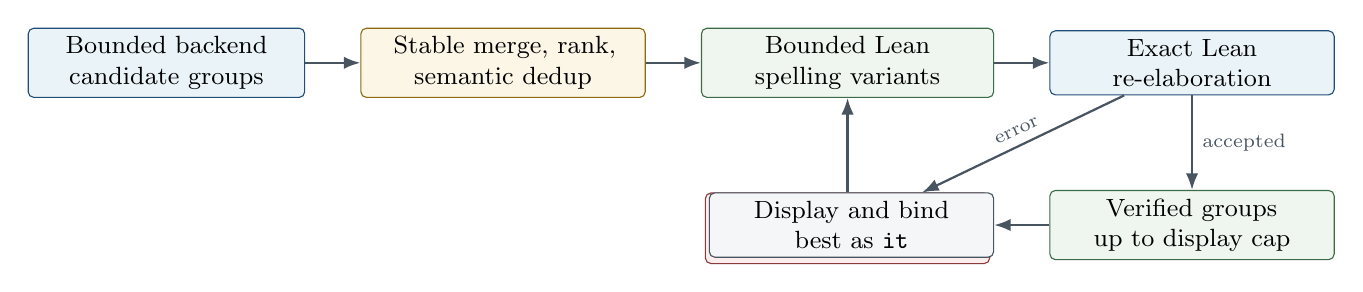
\begin{tikzpicture}[node distance=7mm and 7mm]
  \node[box,text width=33mm] (engine) {Bounded backend\\candidate groups};
  \node[goldbox,right=of engine,text width=34mm] (merge) {Stable merge, rank,\\semantic dedup};
  \node[greenbox,right=of merge,text width=35mm] (render) {Bounded Lean\\spelling variants};
  \node[box,right=of render,text width=34mm] (verify) {Exact Lean\\re-elaboration};
  \node[greenbox,below=12mm of verify,text width=34mm] (accepted) {Verified groups\\up to display cap};
  \node[redbox,below=12mm of render,text width=34mm] (reject) {Reject spelling; try\\next variant/group};
  \node[graybox,left=of accepted,text width=34mm] (bind) {Display and bind\\best as \code{it}};

  \draw[flow] (engine) -- (merge);
  \draw[flow] (merge) -- (render);
  \draw[flow] (render) -- (verify);
  \draw[flow] (verify) -- node[right,note]{accepted} (accepted);
  \draw[flow] (verify) -- node[sloped,above,note]{error} (reject);
  \draw[flow] (reject) -- (render);
  \draw[flow] (accepted) -- (bind);
\end{tikzpicture}}
\caption{The candidate funnel. Internal engine checks and renderer fitting reduce defects, but the exact Lean target is the final gate.}
\label{fig:candidate-funnel}
\end{figure}

\section{Binding results}

Outside prove mode, verified terms are declared in the current Lean environment. They are installed worst-first so the best group becomes the most recent generated value and therefore the friendly bare \code{it}. The new environment IDs and generated history records enter normal undo/replay machinery.

In prove mode, a candidate is not installed as an unrelated global theorem. Leant creates a proof splice applying the candidate to current hypotheses and exposes it as a proof-local \code{itN}. Leaving prove mode clears these splices so they cannot escape the goal context that justified them.

\begin{invariantbox}
Displayed candidates, generated \code{it} values, and prove-mode splices all come from the same verification gate. There is no ``preview'' path that bypasses Lean and later becomes executable state by accident.
\end{invariantbox}

\section{Diagnosing a rejected candidate}

A neutral candidate can be sound in Djex and still fail Lean for several reasons:

\begin{itemize}
  \item the fragment erased a dependency that matters to elaboration;
  \item a provider's implicit argument needs a visible placeholder;
  \item a constructor requires qualification or a different parameter visibility;
  \item eta expansion is required to align a dependent binder;
  \item a pattern is refutable in a forbidden position;
  \item an instance argument cannot be synthesized in the current source context;
  \item a universe or sort relationship was transported opaquely but cannot be reconstructed;
  \item the candidate uses a synthetic premise in a way that cannot be replaced by the source declaration.
\end{itemize}

The correct fix may be a renderer variant, a richer fragment field, a stricter engine projection, or a provider metadata change. Do not weaken final verification.

\chapter{Prove mode and interactive proof synthesis}\label{ch:prove-mode}

\section{Entering prove mode}

The \code{:prove} command establishes a Lean goal and a proof-session state. Subsequent tactic lines are sent to Lean with the current goal state. Responses update displayed goals and the proof environment. Ordinary command history and prove history are related but not identical: proof-local goals and generated splices cannot be replayed as global declarations without their context.

\section{Tactic steps}

A tactic step is authoritative only after the backend returns a new goal state. Leant displays messages, updates the prove counter, and records enough state for proof-local suggestions. A completed proof exits or offers to install the theorem according to command semantics.

\section{Suggestions and synthesis}

\code{:suggest} can ask Lean-oriented automation for tactics or terms. \code{:synth} in prove mode sends the current target through the same fragment/Djex/renderer/verifier pipeline described above. The difference is the source of local premises and the destination of accepted candidates.

The bridge serializes local hypotheses as exact arguments or contexts. A verified candidate may be a function expecting those hypotheses. Leant creates a splice that applies it in the current context, so the user can write \code{exact it} or inspect alternatives. The splice is verified in the proof environment before exposure.

\section{Scope cleanup}

Leaving prove mode clears proof-local \code{it} splices, cached goal translations, and counters tied to the old target. Provider cache entries keyed only by the semantic global world may survive, but any serialized local-provider metadata must not.

A useful invariant is: no value containing a local free variable may enter ordinary global history. The final Lean declaration path enforces this, but prove-state cleanup prevents even friendly-name rewriting from referring to stale locals.

\section{Golden behavior}

The integration corpus includes prove/suggest and synth/prove transcripts. These tests protect not only term correctness but prompt flow, goal display, splice naming, error recovery, and the boundary between proof-local and global generated values.

\chapter{Leant tests and maintenance seams}\label{ch:leant-tests}

\section{Unit tests}

\lpath{test-unit/Spec.hs} is a broad unit suite covering JSON, classifiers, snapshot metadata and publication, replay decisions, fragment parsing and analysis, provider queries and cache behavior, Djex translations, assignment fitting, rendering, candidate grouping, and many regressions around rank-N providers and recursive families. On the pinned branch the suite has 17{,}603 lines and 391 exact \code{testCase} tokens, 390 of which execute as suite cases; its single largest area is the Length/SpinePair behavioral-assessment layer: the current versionless scalar/product startup decoder, contract-only decoding, the current recursive piecewise-affine applicable-domain behavior, the checked handoff, ranking, post-verification sealing, presentation notes, and live execution against the \code{djex-fake-z3} fixture.

Because several production modules are pure, tests can construct exact \code{Frag}, generated AST, provider metadata, and history values without launching Lean. This is where boundary invariants should be tested exhaustively.

\section{Golden integration tests}

The \filepath{test} directory contains command scripts and expected transcripts. The runner starts Leant against the configured Lean backend and compares normalized output. Coverage includes:

\begin{itemize}
  \item basic structural synthesis;
  \item both-engine frontier ordering;
  \item Djinn providers and refutation fallback;
  \item inductive and recursive families;
  \item instance-implicit contexts;
  \item curated library search;
  \item prove-mode synthesis and suggestions;
  \item provider argument rank-N behavior;
  \item constraint closure and quantified providers;
  \item contextual, structural, metadata, and higher-kinded assignments;
  \item visible results depending on exact implicit arguments;
  \item four-, five-, and six-binder rank-N frontiers;
  \item query-closed and recursive rank-N cases.
\end{itemize}

Golden tests are especially appropriate because source spelling, ranking, notes, and result binding are user-visible contracts. Pure tests should still establish the semantic reason for each golden line so formatting changes do not conceal a logic regression.

\section{Natural refactoring seams}

The current code already exposes several safe extraction boundaries:

\begin{enumerate}
  \item Move command parsing and dispatch families out of \code{Main.hs} while keeping one explicit state-transition interface.
  \item Define a typed algebra of backend requests above raw JSON payload construction.
  \item Extract the top-level synthesis phase planner from \code{Main.hs}; keep \code{Fragment}, \code{Engine}, and \code{Render} pure or narrowly effectful.
  \item Separate generated-value management into a module owning mangled names, scanner rewriting, declaration installation, replay recognition, and undo counters.
  \item Preserve \code{ReconstructedSession} as the only installable result of replay, rather than exposing field-by-field mutation.
\end{enumerate}

A refactor should not merge the interactive environment, browse environment, and synthesis environment simply because they all use Lean environment IDs. They have different payload histories and invalidation policies.

\section{Where changes accumulate pressure}

The largest change surfaces are:

\begin{itemize}
  \item \code{Main.hs}: new commands or state fields can touch dispatch, help, replay, reset, transcript, and tests;
  \item \code{Fragment.hs}: a new semantic form touches producer source, parser, all recursive analyses, transformations, and completeness logic;
  \item \code{Engine.hs}: new provider evidence or Djex type structure touches both backend translations and outcome policy;
  \item \code{Render.hs}: new generated terms or fragment binders touch normalization, fitting, naming, variants, and verification tests.
\end{itemize}

The right response is not to avoid these files but to enter them through a checklist. Appendix~\ref{app:change-recipes} provides one.

\begin{summarybox}
Leant's architecture is a sequence of explicit semantic boundaries wrapped in a large interactive orchestrator. The pure modules are already shaped like compiler passes. Maintaining correctness means preserving their metadata contracts and keeping process-local identities out of durable state.
\end{summarybox}

\part{End-to-end traces and maintainer guide}

\chapter{Concrete synthesis traces}\label{ch:traces}

The earlier chapters described each subsystem in isolation. This chapter follows representative requests across all boundaries. The examples are schematic Lean types; exact surface syntax and universe levels vary, but the source paths and state transitions are the ones to inspect in the pinned code.

\section{Trace A: polymorphic identity}

Consider:

\begin{lstlisting}[language=Leanish]
forall {a : Sort u}, a -> a
\end{lstlisting}

\subsection{Lean projection}

The serializer emits an implicit universal binder, then an arrow from \code{a} to \code{a}. Both occurrences carry the same binder key. No depth, unsafe atom, provider, recursive family, or class context is present. The fragment is complete for structural negative evidence.

\subsection{Djex translation}

The bridge maps the binder to a rigid neutral type variable and the arrow to \code{FunctionType}. The original binder visibility is retained in the renderer's slot spine even though the engine type itself does not encode Lean's exact source notation.

\subsection{Djinn}

The positive forall is opened. LJT introduces the arrow antecedent and closes the atomic goal from the local assumption. The proof checker accepts the variable proof under one lambda. Lowering emits a generated lambda with one term binder; the type binder is represented by the surrounding polymorphic scheme rather than an ordinary term lambda.

\subsection{Exference}

The root goal opens the rigid forall scope, introduces one local value, and fills the result hole by selecting that local. Usage is perfect, so the strict lane accepts it. The independent checker reconstructs the variable at the same rigid type.

\subsection{Rendering and Lean verification}

The slot fitter sees one implicit type binder and one term arrow. An idiomatic variant is \code{fun x => x}; a forced explicit type-binder variant is normally unnecessary. Lean elaborates the candidate against the exact goal. Leant installs it as the newest generated \code{it}.

\subsection{Where a regression appears}

If the result is missing, likely boundaries are:

\begin{itemize}
  \item binder keys were not preserved in the serializer/parser;
  \item a rigid variable was incorrectly converted to a flexible one;
  \item generated local scope was lost during simplification;
  \item slot fitting inserted an explicit type lambda unsupported by the target syntax;
  \item verification used a stale Lean environment ID.
\end{itemize}

\section{Trace B: product swap}

Consider:

\begin{lstlisting}[language=Leanish]
forall {a b : Sort u}, a x b -> b x a
\end{lstlisting}

Here \code{x} stands for the product notation in this ASCII document.

\subsection{Projection and neutral type}

The serializer recognizes the product head and emits a product fragment rather than an unsafe nominal application. The bridge maps it to a boxed tuple type or an equivalent declared product constructor view, preserving parameter order.

\subsection{Djinn path}

The formula is \((a \wedge b) \to (b \wedge a)\). Search introduces the input, applies conjunction-left to obtain its fields, applies conjunction-right in reverse order, and returns a checked proof. Lowering may choose a tuple-pattern representation.

\subsection{Exference path}

The result hole selects tuple construction, creating holes of types \code{b} and \code{a}. The input local can be deconstructed. The node builder creates a child lexical scope for pattern-bound fields, fills the holes, and records both uses. The checker validates the case/tuple structure independently.

\subsection{Renderer normalization}

If the generated term uses a tuple pattern directly in a lambda, the renderer can emit the idiomatic form when Lean accepts it or rewrite to a fresh binder plus \code{match}. Binder uniquification must preserve the field order established by the constructor metadata.

This example is an excellent cross-language regression test because a wrong constructor parameter count, a swapped deconstructor scheme, or an incorrect pattern-scope map produces a term that looks plausible but fails final elaboration.

\section{Trace C: sum elimination}

Consider:

\begin{lstlisting}[language=Leanish]
forall {a b c : Sort u}, (a -> c) -> (b -> c) -> Sum a b -> c
\end{lstlisting}

The structural fragment contains two function premises and a binary sum. Djinn translates the sum to a labeled disjunction and uses disjunction-left, creating one branch with an \code{a} assumption and one with a \code{b} assumption. Each branch applies the corresponding function. Proof lowering emits a case expression with exact constructor descriptions.

Exference selects elimination of the sum input, creates branch scopes, and searches each result hole under its branch-local payload. Scope forest correctness matters: the \code{a} value must not be visible in the \code{b} branch. The expression checker reconstructs branch-local schemes and verifies equal result types.

Leant's renderer restores \code{Sum.inl}/\code{Sum.inr} or anonymous constructor notation, normalizes branch patterns, and verifies the match. A branch-scope leak is likely caught by the Exference checker; a wrong Lean constructor spelling is caught by final verification.

\section{Trace D: a live map-like provider}\label{sec:trace-provider}

Suppose the goal is:

\begin{lstlisting}[language=Leanish]
forall {a b : Type u}, (a -> b) -> List a -> List b
\end{lstlisting}

and the current Lean environment exposes a suitable map provider.

\subsection{Structural phase}

Without recursive constructor premises, the engines cannot generally implement mapping. With one-layer list constructors, they may construct only bounded shapes or recurse unsafely; Leant's recursive policy does not invent general recursion. The structural phase therefore usually returns no general term and, because recursive-family projection may be incomplete for elimination, should not immediately refute.

\subsection{Provider discovery}

The provider query records a list-like result head, function relation, and relevant root structure. Lean discovery finds a declaration whose elaborated scheme is morally
\[
  \forall a\,b.\;(a \to b) \to \mathrm{List}\;a \to \mathrm{List}\;b.
\]
The serialized provider fragment records exact constant name, binder visibilities, kinds, contexts, and the correlated assignment vector tying the goal's \code{a} and \code{b} to the provider's binders.

\subsection{Djinn provider lane}

Leant translates the provider to a synthetic premise plus kinded assignment evidence. The formula plan must retain the provider's argument relationship. Djinn can then prove the goal by forwarding the premise at the exact instantiation. The checked proof lowers to a generated global/premise application with visible type applications when necessary.

\subsection{Exference provider lane}

Exference includes the provider in its rated global environment. Selecting it for the \code{List b} result creates holes for the function and list arguments. Locals fill those holes. The occurrence-local assignment is checked and carried into the expression.

\subsection{Renderer}

Synthetic premise lambdas are stripped and replaced with the actual qualified Lean provider name. The renderer decides whether type arguments can be omitted, need \code{_} placeholders, or should be visibly supplied. Several variants may be generated. Lean picks the first that elaborates.

\subsection{Cache behavior}

Repeating the same semantic goal after only installing generated \code{it} values should hit the provider cache. Declaring a new map-like function or instance increments the provider world and forces rediscovery.

\section{Trace E: rank-N forwarding versus elimination}\label{sec:trace-rankn}

Rank-N behavior is easiest to understand by separating two cases.

\subsection{Opaque forwarding}

A goal may merely pass a polymorphic value through unchanged. The nested forall should remain a \code{TypeAtom} or opaque formula symbol. Both engines can prove identity at that atom without opening it. This is why ``all foralls open'' is not the only Djinn plan.

The source renderer does not need to know the internals of the value; it binds and returns it. Final Lean verification confirms exact rank-N type equality.

\subsection{Elimination at an exact assignment}

A different goal consumes a polymorphic argument at a particular type. Ordinary first-order search cannot choose that instantiation soundly. Leant's serializer and provider metadata produce an exact assignment vector; Djex validates kind, closure, correlation, and source scheme; Djinn adds a controlled instantiation axiom or Exference inserts visible type application under a rigid-scope plan.

The generated AST retains the visible type application. Leant maps the neutral type argument back to exact Lean syntax and may insert explicit placeholders for intervening implicit binders. Final elaboration ensures the higher-rank application is legal in the source context.

\subsection{Why assignments are vectors}

For a provider with six correlated binders, independently choosing six locally compatible arguments can create a globally inconsistent scheme. The assignment object is validated as one vector and retained at one provider occurrence. The recent five- and six-binder tests exist to prevent accidental truncation, permutation, or Cartesian explosion in this path.

\section{Trace F: recursive inductive identity}

Consider a goal \code{Tree a -> Tree a} for a recursive family.

The best term is forwarding identity, which requires no unfolding. The serializer therefore retains exact nominal family identity even if it also emits a one-layer recursive schema. Djinn's plan family includes an opaque interpretation that proves forwarding. An implementation that always opens recursive structure could instead generate a large case/rebuild term or mark translation incomplete unnecessarily.

Exference can select the local input directly, with no constructor expansion. Rating and type complexity should prefer this node over a case split. The independent checker sees the same nominal family key on input and output.

The trace demonstrates the dual representation rule: structural exposure is optional search knowledge; opaque identity is mandatory transport knowledge.

\section{Trace G: a sound no-term result}

Consider a purely structural intuitionistic type with no providers, no unsafe atoms, no recursive incompleteness, no contexts outside the supported fragment, and no search budget. A candidate-free Djinn run can produce \code{ProvedUninhabitable}. Leant checks:

\begin{enumerate}
  \item the serializer did not emit depth markers;
  \item every atom is safe for the negative interpretation;
  \item forall and recursive plan families are complete for the observed sites;
  \item exact provider/premise policy is complete for the command mode;
  \item the LJT search finished rather than truncating;
  \item no candidate from library/provider/combined lanes verifies;
  \item the result is not merely an Exference miss or a classical bounded miss.
\end{enumerate}

Only then is the no-term result reported as refutation. This trace should be tested together with near-miss variants that add one \code{FDepth}, unsafe atom, or choice-point budget and therefore downgrade the verdict.

\section{Trace H: backend timeout and replay}

Suppose candidate verification sends a Lean payload that times out.

\begin{enumerate}
  \item The request wrapper raises \code{RequestTimeout} and kills the backend.
  \item The candidate group is not accepted and no generated definition enters history.
  \item \code{ReplState} retains durable imports, snapshot base, history, settings, and Djex-side data, but drops the backend lease.
  \item On the next Lean-requiring command, Leant starts a replacement process.
  \item It restores the snapshot or imports, then replays committed history transactionally.
  \item Only after all steps succeed are the new process and environment IDs installed.
  \item Derived synthesis/provider data tied to process-local serialization is invalidated or rebuilt according to its replay policy.
\end{enumerate}

If replay fails, the partial replacement is discarded. A reset/load command can start another backend without replaying the offending history.

\chapter{Debugging and operational reasoning}\label{ch:debugging}

\section{Classify the symptom before instrumenting}

Most failures fall into one of five observable classes:

\begin{enumerate}
  \item the goal is refused before search;
  \item search returns no candidate;
  \item search returns a candidate that an internal checker rejects;
  \item the renderer produces no Lean spelling;
  \item Lean rejects every spelling or process recovery fails.
\end{enumerate}

These classes correspond to different modules. Start with the earliest wrong artifact rather than the final user message.

\section{Goal refused before search}

Inspect the serializer response and parsed \code{Frag}. Questions:

\begin{itemize}
  \item Is the S-expression syntactically complete and within the depth bound?
  \item Did a dependent product become an unsupported atom or an exact context?
  \item Is a universe/sort binder represented with the expected visibility?
  \item Did a recursive family serialize all constructor domains?
  \item Does \code{fragRefusal} name a deliberate unsupported form or a parser mismatch?
  \item Is the synthesis environment current with respect to interactive history?
\end{itemize}

Add a regression at the \code{Fragment} parser/analysis level before changing engine code.

\section{No candidate from Djinn}

Capture:

\begin{itemize}
  \item the neutral goal and synthetic premise order;
  \item formula plans and completeness flags;
  \item exact assignments retained per plan;
  \item search strategy, remaining choice-point budget, and candidate cutoff;
  \item LJT exhaustion versus truncation;
  \item self-reference diagnostic result.
\end{itemize}

A common cause is a plan that opens a forall needed opaque, or preserves opaque a site needed open. Another is assignment evidence rejected because alias expansion changed the occurrence path. Do not add an unrestricted premise to make the test pass; first establish the missing controlled translation.

\section{No candidate from Exference}

Capture:

\begin{itemize}
  \item root goal after opening leading foralls;
  \item eligible locals/globals/providers and their exact schemes;
  \item queue capacity, steps, depth, identifier exhaustion, and prune counts;
  \item top-scoring nodes around the point the productive path disappears;
  \item strict versus relaxed unused-binder lane;
  \item class obligations and rigid-scope rejections;
  \item checker rejection counts for solved nodes.
\end{itemize}

If queue pruning is nonzero, an ordering change can alter completeness under the bound. A candidate may be generated but then rejected by constraint closure or the independent checker, so ``solved node count'' and ``candidate count'' should be observed separately.

\section{Internal checker rejection}

For Djinn, compare the formula and proof environment at search and check boundaries. The checker should not receive already-erased instantiation evidence. Verify binder freshness after normalization and constructor labels after formula compilation.

For Exference, compare the raw and simplified expressions, reconstructed expected type, residual constraints, rigid provenance, and global schemes. If raw passes but simplified fails, the simplifier likely crossed a binder or visible-type-application boundary. If both fail, the search expansion probably updated the expression and type state inconsistently.

\section{Renderer produces no spelling}

Inspect the generated AST before premise stripping and after each renderer pass:

\begin{enumerate}
  \item Are synthetic premise counts and identities correct?
  \item Are provider occurrences associated with assignment vectors?
  \item Did pattern normalization introduce branch scopes correctly?
  \item Did uniquification find an unbound local or surviving hole?
  \item Does the candidate lambda spine fit the fragment slots?
  \item Did bounded alternative enumeration drop every assignment?
  \item Is a higher-kinded argument being incorrectly treated as a proper fragment?
\end{enumerate}

Write a pure renderer unit test with an explicit generated AST and \code{Frag}. Do not require a full Lean process to reproduce a structural renderer defect.

\section{Lean rejects every spelling}

Retain the exact verification declaration and backend messages. Compare it with:

\begin{itemize}
  \item the original goal text and elaborated target;
  \item binder explicitness and universe parameters;
  \item qualified global/constructor names;
  \item visible type arguments and placeholders;
  \item required instances;
  \item eta-expanded versus non-eta variants;
  \item pattern position restrictions;
  \item noncomputable requirements.
\end{itemize}

A rejection is valuable information: it identifies a mismatch between fragment/renderer assumptions and Lean. The right fix is to enrich or restrict that boundary, not to mark the candidate verified based on Djex alone.

\section{Replay or snapshot failure}

First distinguish transport death from reconstruction failure. Then inspect:

\begin{itemize}
  \item backend configuration and Lake working directory;
  \item snapshot sidecar version, sibling names, sizes, and fingerprints;
  \item synthesis-tooling ABI mismatch;
  \item import probe results;
  \item the first replay history item that fails;
  \item generated \code{it} counter recognition;
  \item whether a reset/load path incorrectly attempted old replay;
  \item whether partial reconstructed fields were installed before failure.
\end{itemize}

The critical postcondition is binary: either a complete replacement session is installed, or the old logical state remains with no live lease. Any mixed state is a correctness bug.

\section{A minimal diagnostic record}

For a hard synthesis regression, capture this compact record in a test fixture or report:

\begin{enumerate}
  \item repository SHAs and selected engine;
  \item exact Lean goal and imports;
  \item parsed fragment summary and negative-evidence ledger;
  \item provider/library names and assignment-vector counts;
  \item neutral Djex goal and premise order;
  \item backend options and progress/evidence;
  \item generated AST before rendering;
  \item rendered variants and Lean error for each attempted variant.
\end{enumerate}

This record is usually enough to reproduce the defect without an entire interactive transcript.

\appendix

\chapter{Module index}\label{app:module-index}

This appendix is a practical source map. It is intentionally selective: it names the files that own contracts or control flow, not every compatibility or test helper.

\section{Djex shared layer}

\begin{longtable}{@{}L{0.43\textwidth}L{0.49\textwidth}@{}}
\toprule
\textbf{File} & \textbf{Read it for} \\
\midrule
\endhead
\dpath{synthesis/src/Language/Haskell/Synthesis/Name.hs} & Checked identifiers, namespaces, definition names, and source-safe naming. \\
\dpath{synthesis/src/Language/Haskell/Synthesis/Kind.hs} & Kind vocabulary, proper/higher kinds, finite kind-tree checks. \\
\dpath{synthesis/src/Language/Haskell/Synthesis/Type.hs} & Neutral type AST, variable rigidity, spines, normalization, substitution, binders. \\
\dpath{synthesis/src/Language/Haskell/Synthesis/TypeAtom.hs} & Alpha-aware opaque nested polytypes and lexical keys. \\
\dpath{synthesis/src/Language/Haskell/Synthesis/Constraint.hs} & Structured class constraints and transformations. \\
\dpath{synthesis/src/Language/Haskell/Synthesis/Declaration.hs} & Shared declarations, constructors, classes, instances, schemes. \\
\dpath{synthesis/src/Language/Haskell/Synthesis/Environment.hs} & Opaque environment authority and strict indexes. \\
\dpath{synthesis/src/Language/Haskell/Synthesis/Inventory.hs} & Search-facing prepared inventory and recursive classification. \\
\dpath{synthesis/src/Language/Haskell/Synthesis/KindInference.hs} & Kind validation and provider assignment kind checking. \\
\dpath{synthesis/src/Language/Haskell/Synthesis/Query.hs} & Query request, contexts, options, cached query, provider evidence. \\
\dpath{synthesis/src/Language/Haskell/Synthesis/Search.hs} & Search batches, progress, completion, truncation reasons. \\
\dpath{synthesis/src/Language/Haskell/Synthesis/Candidate.hs} & Candidate, residual constraints, backend details, rendering boundary. \\
\dpath{synthesis/src/Language/Haskell/Synthesis/Generated.hs} & Common generated expression/pattern/clause AST, scope, simplification. \\
\dpath{synthesis/src/Language/Haskell/Synthesis/Selection.hs} & Bounded stream observation and candidate selection. \\
\dpath{synthesis/src/Language/Haskell/Synthesis/Diagnostic.hs} & Structured validation and search diagnostics. \\
\bottomrule
\end{longtable}

\section{Djinn}

\begin{longtable}{@{}L{0.46\textwidth}L{0.46\textwidth}@{}}
\toprule
\textbf{File} & \textbf{Read it for} \\
\midrule
\endhead
\dpath{djinn/src-core/Language/Haskell/Djex/Djinn.hs} & Stable checked adapter and public session/query operations. \\
\dpath{djinn/src-core/Language/Haskell/Djex/Djinn/Internal/Request.hs} & Query preparation and provider evidence validation. \\
\dpath{djinn/src-core/Djinn/Core.hs} & Plan orchestration, premises, budgets, evidence, deduplication, ranking. \\
\dpath{djinn/src-core/Djinn/Internal/TypeFormula.hs} & Type views, formula compiler, forall/recursive plans, completeness. \\
\dpath{djinn/src-core/Djinn/Internal/LJTFormula.hs} & Formula symbols and proof-term language. \\
\dpath{djinn/src-core/Djinn/Internal/LJT.hs} & Sequent rules, lazy proof search, fairness, budgets, normalization. \\
\dpath{djinn/src-core/Djinn/Internal/ProofCheck.hs} & Independent proof reconstruction. \\
\dpath{djinn/src-core/Djinn/Internal/ProofToGenerated.hs} & Checked proof lowering to shared generated syntax. \\
\bottomrule
\end{longtable}

\section{Exference}

\begin{longtable}{@{}L{0.49\textwidth}L{0.43\textwidth}@{}}
\toprule
\textbf{File} & \textbf{Read it for} \\
\midrule
\endhead
\dpath{exference/src-core/Language/Haskell/Djex/Exference.hs} & Stable checked adapter, projection diagnostics, metrics. \\
\dpath{exference/src-core/Language/Haskell/Exference/Core/Types.hs} & Exference-facing shared type views and substitutions. \\
\dpath{exference/src-core/Language/Haskell/Exference/Core/Unify.hs} & Tagged namespace unification, HK heads, opaque atoms, occurs checks. \\
\dpath{exference/src-core/Language/Haskell/Exference/Core/Internal/ExferenceNode.hs} & Complete search-node state and typed goals. \\
\dpath{exference/src-core/Language/Haskell/Exference/Core/Internal/ExferenceNodeBuilder.hs} & Scope-safe node mutation and fresh allocation. \\
\dpath{exference/src-core/Language/Haskell/Exference/Core/Internal/Exference.hs} & Queue scheduler, expansion, pruning, completion, lazy trace. \\
\dpath{exference/src-core/Language/Haskell/Exference/Core/Expression.hs} & Annotated generated expression and compatibility patterns. \\
\dpath{exference/src-core/Language/Haskell/Exference/Core/ExpressionCheck.hs} & Independent bidirectional reconstruction and constraint check. \\
\bottomrule
\end{longtable}

\section{Djex facade and frontends}

\begin{longtable}{@{}L{0.42\textwidth}L{0.50\textwidth}@{}}
\toprule
\textbf{File} & \textbf{Read it for} \\
\midrule
\endhead
\dpath{src/Language/Haskell/Djex.hs} & Unified backend facade and capability matrix. \\
\dpath{src/Language/Haskell/Djex/HaskellSrc.hs} & Source declaration/type conversion and rendering bridge. \\
\dpath{src/Language/Haskell/Djex/Package.hs} & Package/tool discovery and package-level loading. \\
\dpath{src/Language/Haskell/Djex/REPL.hs} & Unified interactive orchestration. \\
\dpath{src/Language/Haskell/Djex/REPL/Scope.hs} & Visibility, qualification, ambiguity, imports/exports. \\
\dpath{src/Language/Haskell/Djex/REPL/Workspace.hs} & Module graph and workspace reload behavior. \\
\dpath{src/Language/Haskell/Djex/CLI.hs} & Process modes and command-line entry. \\
\bottomrule
\end{longtable}

\section{Leant}

\begin{longtable}{@{}L{0.38\textwidth}L{0.54\textwidth}@{}}
\toprule
\textbf{File} & \textbf{Read it for} \\
\midrule
\endhead
\lpath{src/Main.hs} & Interactive state, commands, ordinary Lean execution, synthesis phase entry, verification, generated values, prove mode. \\
\lpath{src/Leant/Backend.hs} & Child process, framing, timeout/death errors, discovery. \\
\lpath{src/Leant/Json.hs} & Protocol JSON parser and encoder. \\
\lpath{src/Leant/Classify.hs} & Multiline lexical classifier. \\
\lpath{src/Leant/Session/Replay.hs} & Transactional replay accumulator. \\
\lpath{src/Leant/Session/Snapshot.hs} & Snapshot family, sidecar, fingerprint, publication. \\
\lpath{src/Leant/Synth/Fragment.hs} & Lean serializer, parser, fragment grammar, provider and completeness metadata. \\
\lpath{src/Leant/Synth/ProviderCache.hs} & Semantic provider key and world-generation cache. \\
\lpath{src/Leant/Synth/Replay.hs} & Derived synthesis replay decision. \\
\lpath{src/Leant/Synth/Engine.hs} & Djex translation, search lanes, providers/library, merge, evidence. \\
\lpath{src/Leant/Synth/Render.hs} & Premise stripping, pattern normalization, fitting, variants, Lean text. \\
\filepath{src/Leant/Synth/Observability.hs} (current branch) & \code{CandidateRenderingRoute}, \code{VerificationFailureClass}, \code{LeantSynthesisMetric}: the typed-route eligibility vocabulary. \\
\bottomrule
\end{longtable}

\chapter{Important bounds and invariants}\label{app:limits}

The following values describe the pinned revisions. They are part implementation limits, part denial-of-service boundaries, and part search-policy contracts. Before changing one, find every validator, serializer, plan enumerator, renderer alternative bound, and test that assumes it.

\begin{longtable}{@{}L{0.40\textwidth}L{0.15\textwidth}L{0.35\textwidth}@{}}
\toprule
\textbf{Bound} & \textbf{Value} & \textbf{Why it exists} \\
\midrule
\endhead
Djex provider-instantiation candidates & 32 & Bounds exact evidence enumeration and validation. \\
Djex provider assignments & 32 & Bounds correlated alternatives per request/provider set. \\
Arguments in one provider assignment & 6 & Keeps exact vector validation and rank-N frontiers finite; covered by six-binder regressions. \\
Observed kind arity & 64 & Prevents unbounded higher-kinded head trees from source input. \\
Kind-tree node observation & 129 & Sentinel-style bound corresponding to a finite binary observation around the arity limit. \\
Leant exact forall-domain tags & 128 & Bounds serialized exact provider-domain metadata. \\
Djinn quintuple frontier cap & 512 per orientation & Bounds open/opaque plan combinations while remaining complete through eleven sites for quintuple choices. \\
Exference queue capacity in Leant lane & 1024 & Keeps live provider/library search operational; exact pruning is reported. \\
Leant backend candidate window & 60 & Gives renderer/verification room after deduplication and rejection. \\
Leant combined verification frontier & 24 & Bounds cross-engine semantic groups entering expensive Lean verification. \\
Leant attempted result groups & 12 & Bounds verification work and user-visible latency. \\
Leant shown successful groups & 5 & Keeps interactive output focused while retaining alternatives. \\
Backend stderr capture & newest 64 KiB (bytes) & Continuous capture on a dedicated thread with a truncation flag; the death-path drain waits only briefly, so crash diagnostics cannot hang reconstruction. \\
\bottomrule
\end{longtable}

\section{Invariant checklist}

\begin{enumerate}
  \item Every public authority has a validating constructor and hidden representation.
  \item Every finite authority observes lazy input through a bound plus sentinel, never an unbounded \code{length} assumption.
  \item Type atoms preserve alpha identity and free-variable hygiene while blocking structural decomposition.
  \item Environment source order and all strict indexes advance transactionally.
  \item Search evidence is represented separately from completion/truncation.
  \item Djinn negative evidence requires complete translation and exhaustive unbudgeted search.
  \item Exference never reports logical uninhabitability from heuristic exhaustion.
  \item Every Djinn proof and Exference solved expression passes an independent internal checker.
  \item Every Leant candidate passes exact Lean elaboration before display or installation.
  \item Every lossy Lean-to-fragment projection records incompleteness explicitly.
  \item Provider assignments are exact correlated vectors with kind and occurrence provenance.
  \item Synthetic premises have stable identities and are removed structurally by the renderer.
  \item Process-local Lean environment IDs never survive backend replacement without replay.
  \item Session reconstruction is all-or-nothing.
  \item Generated \code{it} bindings do not invalidate provider discovery, but ordinary declarations do.
  \item Proof-local generated values never enter global history with free locals.
\end{enumerate}

\chapter{Change recipes}\label{app:change-recipes}

\section{Adding a new shared type constructor}

Suppose Djex must represent a new type form rather than preserving it as a \code{TypeAtom}.

\begin{enumerate}
  \item Add the constructor and smart constructors in the shared type layer.
  \item Define equality, ordering/key behavior, free variables, binder traversal, substitution, alpha normalization, finite-width validation, and source rendering.
  \item Decide how it participates in function/application/constructor spines and kind inference.
  \item Update environment and inventory traversal, synonym expansion, and recursive classification.
  \item In Djinn, add a one-layer \code{TypeView} case and make polarity/opacity/completeness explicit. Update formula symbols, constructor descriptions, proof checking, and lowering only if structurally supported.
  \item In Exference, update unification, zonking, occurs checks, rigid scope, node expansions, simplification, and the independent checker.
  \item Update the generated AST only if terms need a new elimination/introduction form; do not add one merely because the type is new.
  \item Update source frontends and Leant's fragment translation if the form crosses that bridge.
  \item Add negative tests where the form is unsupported or opaque; add positive tests for forwarding and structural use separately.
\end{enumerate}

\section{Adding a new \code{Frag} constructor}

This is one of the highest-risk changes because \code{Frag} is simultaneously search, render, and evidence data.

\begin{enumerate}
  \item Extend the embedded Lean serializer and give the form an unambiguous S-expression tag and bounded fields.
  \item Extend the Haskell parser with malformed, truncated, and width tests.
  \item Define free variables, binder spines, recursion keys, unsafe atoms, provider openness, exact contexts, depth behavior, and source-display summaries.
  \item Decide whether the form is structurally translated, transported opaquely, or refused per engine.
  \item Add a completeness rule: can hiding this form invalidate refutation?
  \item Update library/provider serializers and relevance filtering if declarations can contain the form.
  \item Update fragment-to-Djex translation and exact assignment metadata.
  \item Update renderer fitting, binder domains, constructor metadata, and source variants.
  \item Add a pure round-trip fixture, engine tests, renderer tests, final Lean golden tests, and a negative-evidence near miss.
\end{enumerate}

\section{Adding a new generated expression form}

\begin{enumerate}
  \item Extend shared \code{Generated} validation, scope traversal, free locals, simplification, application spines, equality/deduplication, and render diagnostics.
  \item Add production and checking to each backend separately. Search construction alone is insufficient.
  \item In Exference, extend annotated expression conversion and bidirectional checking.
  \item In Djinn, extend proof lowering only when a checked proof rule justifies the form.
  \item Extend Leant's pattern normalization, uniquification, premise substitution, fitting, and both idiomatic/explicit renderers.
  \item Verify every source target; a Haskell-renderable form may not have direct Lean syntax.
\end{enumerate}

\section{Adding provider metadata}

\begin{enumerate}
  \item Identify whether the data is semantic evidence, renderer evidence, ranking input, or diagnostic text. Use separate fields/types when it serves more than one role.
  \item Serialize it from elaborated Lean declarations with exact occurrence identity.
  \item Bound vectors and trees at the parser boundary.
  \item Include it in semantic cache keys only if changing it can change provider eligibility or assignments.
  \item Validate it against Djex schemes and kinds before search.
  \item Retain enough provenance through formula plans or Exference nodes.
  \item Match it occurrence-locally in the renderer; do not apply one provider-wide guess to every occurrence.
  \item Add correlated-assignment tests with repeated variables and higher-kinded heads.
\end{enumerate}

\section{Changing a search bound}

A bound change is a semantic change whenever progress or result order is user-visible.

\begin{enumerate}
  \item Find the validating smart constructor and the runtime cutoff.
  \item Check whether a sentinel observation relies on \(N+1\).
  \item Check whether budgets are global, per plan, per lane, or per queue.
  \item Update exact truncation reasons and tests.
  \item Measure first-candidate latency, result ordering, checker rejection, and negative-evidence behavior.
  \item Ensure Leant does not reinterpret a formerly truncated run as exhaustive after only changing display limits.
\end{enumerate}

\section{Adding a Leant REPL command}

\begin{enumerate}
  \item Add help and command parsing without colliding with Lean source classification.
  \item Declare whether the command requires a live backend and whether old history must be replayed first.
  \item Define state effects by ownership domain: durable history, process lease, derived cache, provider world, generated values, prove state, transcript.
  \item Decide undo semantics and whether the command establishes a new reconstruction root.
  \item Route all output through \code{emit}.
  \item Test success, backend death, timeout, bad response, reset/replay interaction, and noninteractive script output.
\end{enumerate}

\section{Changing snapshot format}

\begin{enumerate}
  \item Increment the sidecar format version or define a backward-compatible parser explicitly.
  \item Include every sibling artifact in name/size/fingerprint validation.
  \item Update the synthesis-tooling ABI when serializer or required prelude semantics change.
  \item Preserve old snapshot files until the new family has been fully written and validated.
  \item Test publication failure at every rename step, especially on Windows.
  \item Test that an incompatible snapshot is rejected before starting replay from it.
\end{enumerate}

\section{Extracting code from \code{Main.hs}}

Use state-transition boundaries rather than arbitrary line ranges.

\begin{itemize}
  \item A command module should receive an explicit capability/state view and return either a complete state replacement or a command result describing effects.
  \item Backend request construction should return typed payload/result values; raw JSON should remain in a narrow protocol layer.
  \item Generated-value management can own mangled names, lexical rewriting, installation order, replay recognition, and counters.
  \item Synthesis orchestration can own phase order and outcome merge while delegating exact Lean effects to callbacks.
  \item Transactional reconstruction should continue to return one installable \code{ReconstructedSession}; do not expose partial field setters.
\end{itemize}

\chapter{Glossary}\label{app:glossary}

\begin{description}[style=nextline,leftmargin=0pt,labelsep=0pt]
  \item[Authority type] An opaque type whose values certify that a validation procedure has succeeded.
  \item[Candidate group] Several Lean source spellings representing one semantic generated candidate.
  \item[Checked request] A backend-private request tied to a validated session and exact environment.
  \item[Completeness ledger] Metadata recording every projection, plan, or budget condition relevant to negative evidence.
  \item[Exact context] A class/instance binder represented with structured class head and arguments rather than an ordinary arrow.
  \item[Generated AST] Djex's common scoped expression and pattern language produced by both engines.
  \item[Kinded assignment] A correlated provider-instantiation vector retaining each argument's exact kind.
  \item[LJT] The contraction-free intuitionistic sequent-calculus family used by Djinn's proof search.
  \item[Opaque forwarding] Treating a complex type as one atom so a value can be passed unchanged without opening unsupported structure.
  \item[Prepared inventory] A checked search-facing projection of a Djex environment.
  \item[Provider] A live or curated declaration whose scheme may be applied to construct the current goal.
  \item[Provider world] Leant's generation number for the semantic universe of discoverable declarations and instances.
  \item[Residual constraint] A class obligation remaining after a candidate's expression has been reconstructed.
  \item[Rigid variable] A type variable that represents a scoped constant and cannot be solved by ordinary unification.
  \item[Slot] Leant's view of a leading Lean binder, retaining arrow/forall/instance and visibility behavior for fitting.
  \item[Type atom] An alpha-aware opaque nested type region that preserves variables but blocks structural decomposition.
  \item[Verification gate] Final Lean elaboration of a rendered candidate against the exact original target.
\end{description}

\chapter{Pinned source entry points}\label{app:sources}

\section{Repository roots}

\begin{itemize}
  \item Djex pinned tree: \href{https://github.com/VladimirReshetnikov/Djex/tree/da1dd7a316975aa8a9c59022d7dbee879f67a168}{\nolinkurl{github.com/VladimirReshetnikov/Djex/tree/da1dd7a...}}
  \item Leant pinned tree: \href{https://github.com/VladimirReshetnikov/Leant/tree/c3e53cee1a19a21930a64a5cb74e3926c29a7eab}{\nolinkurl{github.com/VladimirReshetnikov/Leant/tree/c3e53ce...}}
  \item Leant's submodule declaration: \lpath{.gitmodules}
  \item Leant's multi-package build: \lpath{cabal.project}
\end{itemize}

\section{Fastest route for a code review}

For a change in synthesis behavior, review in this order:

\begin{enumerate}
  \item public/bridge type changes in Djex shared modules;
  \item opaque smart constructors and their tests;
  \item the selected backend adapter and independent checker;
  \item Leant fragment serializer/parser and completeness analyses;
  \item Leant engine translation and provider assignment construction;
  \item Leant renderer variants and final Lean golden tests;
  \item evidence/progress handling and regression cases for candidate-free outcomes.
\end{enumerate}

For a change in interactive behavior, review:

\begin{enumerate}
  \item command parsing and help;
  \item backend requirement/replay policy;
  \item complete \code{ReplState} transition;
  \item undo/reset/load/snapshot behavior;
  \item provider and derived-environment invalidation;
  \item transcript and noninteractive golden output.
\end{enumerate}

\chapter*{Conclusion}
\addcontentsline{toc}{chapter}{Conclusion}

Djex and Leant are best understood not as one theorem prover and one shell, but as a chain of explicitly checked translations. Djex gives two very different engines a common semantic perimeter. Djinn contributes proof-producing structural search and carefully qualified negative evidence. Exference contributes ranked typed-hole search, richer source-oriented application behavior, and a separate reconstruction checker. Leant projects elaborated Lean goals into a bounded fragment, plans structural/library/provider lanes, preserves exact instantiation metadata, reconstructs source syntax, and asks Lean to decide the final claim.

The codebase's strongest recurring idea is that uncertainty should have a type or a flag rather than an optimistic comment. Opaque regions remain opaque. Truncation is recorded. Exact assignments carry provenance. Search proposals are checked. Process-local IDs are reconstructed transactionally. A candidate-free heuristic run remains a candidate-free heuristic run. These disciplines are what allow the system to grow toward more powerful synthesis without silently converting approximation into unsoundness.

For maintainers, the practical rule is equally simple: follow the representation ladder. At every boundary, ask what information was retained, what was intentionally hidden, what validator established the next authority, and which later checker closes the remaining gap. The answer usually points directly to the right module and the right regression test.

\end{document}
